\documentclass{ieeeaccess}
\usepackage{cite}
\usepackage{amsmath,amssymb,amsfonts}
\usepackage{algorithmic}
\usepackage{graphicx}
\usepackage{textcomp}
\usepackage{tikz}
\usepackage{import}
\usepackage{svg}
\usepackage{float}
\usepackage{amsmath}
\usepackage{fourier} 
\usepackage{array}
\usepackage{makecell}
\usepackage{multirow}
\usepackage{hyperref}
\usepackage{colortbl}

% \usepackage{subcaption}
\renewcommand\theadalign{bc}
\renewcommand\theadfont{\bfseries}
\renewcommand\theadgape{\Gape[4pt]}
\renewcommand\cellgape{\Gape[4pt]}

\newlength{\Oldarrayrulewidth}
\newcommand{\Cline}[2]{%
  \noalign{\global\setlength{\Oldarrayrulewidth}{\arrayrulewidth}}%
  \noalign{\global\setlength{\arrayrulewidth}{#1}}\cline{#2}%
  \noalign{\global\setlength{\arrayrulewidth}{\Oldarrayrulewidth}}}
\DeclareMathOperator*{\argmin}{argmin} 
\DeclareMathOperator*{\argmax}{argmax} 
\DeclareMathOperator*{\concat}{||} 

\NewSpotColorSpace{PANTONE}
\AddSpotColor{PANTONE} {PANTONE3015C} {PANTONE\SpotSpace 3015\SpotSpace C} {1 0.3 0 0.2}
\SetPageColorSpace{PANTONE}%
\def\BibTeX{{\rm B\kern-.05em{\sc i\kern-.025em b}\kern-.08em
    T\kern-.1667em\lower.7ex\hbox{E}\kern-.125emX}}
\begin{document}
\history{Date of publication xxxx 00, 0000, date of current version xxxx 00, 0000.}
\doi{10.1109/ACCESS.2017.DOI}

\title{DetectBERT: Toward a versatile architecture for source code vulnerability detection}
\author{\uppercase{Hoai-Chau Tran}\authorrefmark{1, 3},
\uppercase{Anh-Duy Tran\authorrefmark{4}, and Kim-Hung Le}.\authorrefmark{2,3}}
\address[1]{University of Science, Ho Chi Minh City, Vietnam (e-mail: author@boulder.nist.gov)}
\address[2]{University of Information Technology, Ho Chi Minh City, Vietnam (e-mail: author@lamar.colostate.edu)}
\address[3]{Vietnam National University, Ho Chi Minh City, Vietnam}
\address[4]{imec-DistriNet, KU Leuven, Leuven, Belgium}
\markboth
{Author \headeretal: Preparation of Papers for IEEE TRANSACTIONS and JOURNALS}
{Author \headeretal: Preparation of Papers for IEEE TRANSACTIONS and JOURNALS}

\corresp{Corresponding author: First A. Author (e-mail: author@ boulder.nist.gov).}

\begin{abstract} 
Detecting vulnerabilities in source code using learning-based approaches has gained significant attention in recent years. While GNN-based deep learning methods have shown promising results in detecting vulnerabilities, GNNs have limitations due to inductive biases toward predefined graph structures and local connectivity,  a common solution for this issue is to combine different graph structures to provide the GNN models with more context about the relationship between statements. However, the process of constructing graphs is challenging and hard to reproduce for multiple programming languages.  To overcome the limitations of GNN-based approaches, we propose a highly versatile approach called DetectBERT,  which uses self-attention mechanisms to detect vulnerable code at the statement level in Python without requiring any pre-defined graph structures. In essence, DetectBERT consists of two BERT-based models which serve as a feature  extractor and classifier that can learn contextual interactions between statements in  code snippets/functions. To evaluate the effectiveness of our approach,  a new dataset was created from two different public datasets, both of which contain multiple commits from real-world open-source projects. Given a Python file, the data processing pipeline involves extracting and normalizing all statements and  grouping them into function gadgets, resulting in a dataset that contains over 21,000 processed samples.  The empirical results demonstrate that DetectBERT can outperform other GNN-based methods that use Control Flow Graph as the underlying graph structure. Specifically, for statement-level vulnerability detection, the best DetectBERT model achieved an F1 score of 70.34\%, precision of 68.80\%, and recall of 75.83\%, which outperforms GNN-based models with the best hyperparameter settings ( GCN had the best  F1 score of 47.18\%, precision of 40.26\%, and recall of 64.71\% and GAT  had the best F1 score of 50.50\%, precision of 43.98\%, and recall of 67.12\%). 
\end{abstract}

\begin{keywords}
Enter keywords or phrases in alphabetical 
order, separated by commas. For a list of suggested keywords, send a blank 
e-mail to keywords@ieee.org or visit \underline
{http://www.ieee.org/organizations/pubs/ani\_prod/keywrd98.txt}
\end{keywords}

\titlepgskip=-15pt

\maketitle

\section{Introduction}\label{sec:I}
\par % Paragraph nói về ngữ cảnh của các nguy cơ trong code (vulnerability) có khả năng dẫn tới các nguy cơ về an toàn thông tin
Detecting vulnerabilities in source code is a critical task in modern software development. It helps ensure the safety and security of software users since attackers can exploit vulnerabilities embedded in source code \cite{cwe22,cwe352,cwe601,cwe79,cwe94,CWE-77,CWE-89} to compromise the integrity of an application or system. To identify potential security vulnerabilities in the early stages of the development process, source code vulnerability detection (SVD) is often performed as part of Static Application Security Testing (SAST). However, traditional SVD approaches using  rule-based \cite{rule_tool1, rule_tool2, rule_tool3, rule_tool4, rule_tool5, rule_tool6, coverity} methods can be error-prone due to the complexity and variability of real-world source code in different projects \cite{sast_tools_study}. In recent years, deep learning (DL)-based approaches \cite{Linevd, MVD, vuldeekeeper, SySeVR, VulDeeLocator, DeepWukong, VUDENC, func_level_1, func_level_2, func_level_4, devign, Are, vuldeepeeker2} have shown promising results in adapting to real-world code changes and providing wider coverage in detecting vulnerable code.

 

\par % VIết vể các challenge hiện tại
While DL-based approaches for detecting vulnerable code have shown great promise, there are still challenges to overcome before they can be effectively applied to real-world software development. One major obstacle is the issue of robustness and generalization. Since deep learning models require a significant amount of data to train, the quantity and quality of datasets used can greatly affect their performance. If the dataset quality is low, it can lead to inaccurate predictions of vulnerable patterns and an increased rate of false negatives for unseen data. One factor that can harm the quality of the dataset is the presence of duplicated samples  in both training and testing data, which can cause data leakage and artificially inflate reported results \cite{vuldeekeeper, VUDENC, SySeVR, Are}. Furthermore, some datasets \cite{devign, sard, SATE} do not accurately reflect the real-world distribution of vulnerable code, where non-vulnerable code makes up a larger portion of a software codebase. Additionally, the models can be confused by the presence of user-defined variables, functions, classes, and strings in the source code. These factors, combined with the presence of duplicated data, can cause the model to simply "memorize" trained data instead of actually learning vulnerable patterns.

\par Another limitation of recent DL-based approaches is that they often overlook the fact that a vulnerable pattern can exist in just a few lines of code. Instead, they focus on a higher level of granularity, such as function-level \cite{Are, devign, func_level_1,func_level_2,func_level_4}, slice-level \cite{VUDENC, vuldeepeeker2, SySeVR, VulDeeLocator,vuldeekeeper}, or even file-level \cite{File_level_1, File_level_2, File_level_3, file_level_4}. This can make it difficult and time-consuming for developers to identify the specific source of the problem and can result in missed vulnerabilities, longer review times, and increased effort to detect and remediate the issue.
While the manual labeling process requires a deep understanding of the code structure and the programming language itself, the most promising solution used in previous studies \cite{Linevd, MVD}, is to use commit history from open-source repositories to identify fixes for vulnerabilities and label the deleted lines as vulnerable. However, this approach also has limitations. Many commits are not directly related to the vulnerability or only resolve a portion of the problem. Also, some changes in the code are irrelevant to the vulnerability (adding/removing tabs, trailing spaces, line breaks, and comments).


\par % Viết về tổng quan solution để giải quyết
    Given the above problems, there were efforts to resolve them. To deal with the unrealistic data distribution, previous works have used real-world code from open-source projects to create their own dataset\cite{devign, Are, Linevd, VUDENC, cvefixes} instead of synthesis or semi-synthesis datasets\cite{sard, SATE, Draper}, further preprocess steps are also conducted to normalize user-defined names into symbolic representations\cite{vuldeekeeper, vuldeepeeker2, DeepWukong,SySeVR,VulDeeLocator}. By selecting data from open-source projects and normalizing source code, the issue of data duplication is partially addressed. However, it is still unavoidable as some portions of the code from different repositories may resemble each other due to code reuse and sharing practices. 
\par To improve the prediction results at a more detailed, statement-level granularity, previous studies\cite{MVD, Linevd, IVDetect} have employed graph data structures, where each statement is represented as a node, then feature vectors are extracted from each node using either static\cite{glove, doc2vec, word2vec} or dynamic embedding\cite{codebert} methods. After the feature extraction process, node/graph classification is performed by combining different types of graphs (Control Flow Graph, Data Dependency Graph, Program Dependency Graph, Call Graph, etc.) with supplementary information  and using a GNN (Graph Neuron Network) architecture such as Graph  Attention Network (GAT)\cite{GAT},  Graph Convolution Network (GCN)\cite{GCN} to learn the relationships and interaction between nodes. These approaches using GNNs have achieved state-of-the-art performance for the SVD task in recent years.

\par Although GNNs have demonstrated promising empirical results compared to other methods, they still have some limitations. These models are often constrained by inductive biases, such as local connectivity and predefined graph structures, which restrict their ability to identify more complex patterns and learn from distant statements because of missed connections. To overcome this limitation, there are two common strategies: increasing the number of layers in the GNN model or combining different graph structures to capture more features from distant code statements. The latter strategy is often preferred in previous studies \cite{Linevd, DeepWukong, MVD, IVDetect, Are} since increasing the number of layers in GNNs can harm the model's performance due to the over-smoothing \cite{over_smooth} and over-squashing\cite{over_squash} problems in GNN  architectures. 

However, constructing graphs for multiple programming languages is a challenging and non-scalable process due to various reasons. One of the major challenges is that programming languages keep evolving, with new constructs and features being added in newer versions. Consequently, developing graphs that are compatible with multiple versions of a language can be difficult. For instance, the Abstract Syntax Tree (AST) module of Python 2 is incapable of parsing AST for Python 3 code, and vice versa. In addition, different programming languages have distinct syntaxes and semantics, which require more effort to reconstruct informative graphs for each programming language. Moreover, the process of constructing different graph structures heavily relies on available tools in each programming language, thus, most recent previous works \cite{Are,devign,DeepWukong,Linevd,MVD,IVDetect} have exclusively focused on building SVD solutions for C/C++  due to  the extensive ecosystem of tools and libraries available\cite{c_tool1,c_tool2,ctool3,ctool4}. To address the challenges of GNNs, a new approach is necessary to capture the relationship between statements without relying on any pre-defined graph structures.


\par % Dẫn vào bài báo và đóng góp của em
In this paper, we present DetectBERT, a deep learning-based approach that can provide statement-level predictions without extracting graphs and can be used over multiple programming languages. In general, the architecture of DetectBERT consists of  two transformer encoder (BERT-based) models which are utilized to extract feature vectors (feature extractor) and learn the complex relationships between statements in code snippets or functions (classifier). The motivation behind this idea is that  the transformer's encoder architecture is actually a special case of graph neural network (GNN), where nodes are globally interconnected \cite{transformer2graph}, and self-attention layers in the encoder model enable learning of the interactions between nodes. This is similar to the message-passing mechanism of GNNs, where weighted connections are established between every pair of nodes in the graph. Using this approach, we can avoid relying on any specific set of tools in any programming language and leverage large amounts of data from real-world open-source projects to form more connections between nodes without a predefined graph structure. Moreover, there are many BERT-based models \cite{sBERT,codebert, minilm,mpnet, zhou2023codeBERTscore} that are pre-trained on large amounts of code corpus in different programming languages, making it easier to scale our architecture to perform SVD tasks for multiple programming languages. The motivation and inner workings of our model will be discussed in sections \ref{sec:motivation} and \ref{sec:ME}, respectively.

\begin{figure}[h]
    \centering
    \includegraphics[width=85mm]{sample.png}
    \caption{Our model has identified a code sample that is susceptible to CWE-601 (URL Redirection to Untrusted Site ) vulnerability, with a stronger indication of vulnerability represented by a darker red line. The Python statement that lies between lines 114 to 118  assigns the value of the `redirect\_field\_name` parameter received in the request to the `oidc\_login\_next` session variable. This variable is then used later to redirect the user after the authentication process is complete. If the value of `redirect\_field\_name` is controlled by an attacker, they can potentially set it to a malicious URL and trick the user into visiting it. This is known as an open redirect vulnerability. To prevent this vulnerability, validating the `redirect\_field\_name` parameter is important before using it to set the `oidc\_login\_next` variable. One way to do this is to only allow redirection to specific, trusted URLs. Another approach is to use a whitelist of allowed values for the `redirect\_field\_name` parameter.}
    \label{fig:sample}  
\end{figure}
\par While most previous works build their model for only C/C++, Python is chosen as the main programming language for the SVD task, the reason behind this decision is Python's syntax is closer to natural language for which transformers models perform very well\cite{Embeds_comparison}. On the other hand, Python does not receive a lot of attention in recent works despite its popular usage in many fields (artificial intelligence, web development, automation and system administration, IoT development, game development, etc.) due to its ease of use, versatility, and availability of many libraries and modules. The data used in this work is got from two public datasets which are CVEFixes\cite{cvefixes} and VUDENC\cite{VUDENC}, both of which originated from GitHub commits that are used to patch issues related to vulnerabilities in different open-source projects, we also introduce our own labeling criteria to reduce false positive ground truth. To make the model more robust to adversarial attacks, all user-defined names such as variables and functions are normalized into generic names, then all statements are extracted and labeled based on changes in collected commits. More information about the data processing and labeling process will be provided in section ~\ref{sec:FE}.

\par In summary, this paper makes the following contributions:
\begin{itemize}
\item  We propose DetectBERT,  an architecture that can carry out statement-level SVD for Python source code  by stacking two BERT-based models as a feature extractor and a classifier. By using the self-attention mechanism  in transformer enocders\cite{attention}, the model  can learn connections and relationships among statements in a function  without using any predefined graph structure.
\item  Experiments with the aim to evaluate the effectiveness of DetectBERT are conducted by comparing it with other GNN-based architectures. To the best of our knowledge, there is no previous work that has constructed a graph dataset for Python. Hence, we have created our own version using Control Flow Graphs (CFGs) as the underlying data structure. The empirical result shows that DetectBERT can outperform the GNN-based approaches in every metric.
\item  Since the datasets \cite{VUDENC, cvefixes, devign} used  in this  paper  are not originally  built for statement-level classification,  a new data preprocessing pipeline was built  to extract, normalize and label Python statements. Due to the lack of domain knowledge,  the commits history from  open-source projects is also utilized for the labeling process, however, to reduce the number of false positive ground-truth labels,  we also introduce our own criteria to filter commit changes  that are irrelevant to the vulnerable pattern and reduce the duplication rate in the dataset. 
\item  Although our solution was first intended to build for Python, an additional experiment on C/C++ code was also conducted to demonstrate the versatility of our architecture. The experiment is conducted on the Devign dataset \cite{devign} which is originally created for function-level. In order to perform statement-level for each sample,  C/C++ statements are also extracted and labeled based on the added and deleted lines in each sample's commits. The experiments showed competitive results compared to other GNN-based approaches proposed in \cite{Linevd} with the same objective. 
\item To further advance the field and enable future research, we have made our implementations including the whole pipeline (data preprocessing, training, and inference), datasets, and models publicly available on \href{https://github.com/Edwin372/DetectBERT}{GitHub} and \href{https://huggingface.co/EddieChen372/DetectBERT}{Huggingface Hub}. This will allow other researchers and practitioners to reproduce our experiments and build upon our work. 
\end{itemize}
\section{Background and motivation}
This section will give a brief background about Graph Neural Networks (GNNs) and BERT-based models and discuss how these architectures have been applied to perform SVD in recent years.
\subsection{BERT-base models}
BERT \cite{bert} and its variant models \cite{albert,distilbert}  have become increasingly popular in recent years for natural language understanding (NLU)\cite{bert}. At the heart of these models lies the transformer encoder layers, which use a multi-head self-attention mechanism. Further details about self-attention layers and other components such as layer normalization\cite{layer_norm}, residual connection, and full-connected feed-forward neuron network, can be found in the very famous study\cite{attention} by Vaswani et al. Essentially, given a sentence that has been tokenized into $n$ tokens, we can represent the embedding matrix for that sentence as $X\in \mathbb{R}^{n \times d}$ where $d$ is the hidden size of the embedding vectors. The entire process can be formulated as follows:
\begin{equation}
\text{MultiHead}(Q,K,V) = \text{Concat}(head_1,...,head_h)W^O
\end{equation}
\begin{equation}
\text{head}_i = \text{Attention}(XW_i^Q,XW_i^K,XW_i^V)
\end{equation}
\begin{equation} \label{equa:self_attention}
\text{Attention}(Q,K,V) = \text{softmax}\left(\frac{QK^T}{\sqrt{d_k}}\right)V
\end{equation}

Here, $Q$, $K$, and $V$ are the matrices obtained from the input sequence, and $W_i^Q$, $W_i^K$, and $W_i^V$ are the trainable weight matrices for the $i^{th}$ attention head. The output of each attention head is concatenated, and the resulting matrix is multiplied by a weight matrix trainable $W^O$ to obtain the final output. The $\text{softmax}$ function is applied to the scaled dot-product of $Q$ and $K$ to calculate the attention scores. The constant $d_k$ is the dimensionality of the key vectors.

\par In the context of detecting vulnerable code, it is common to benefit from transfer learning by utilizing pre-trained BERT models \cite{codebert} as a feature extractor layer\cite{Linevd, Embeds_comparison}, which generates a dynamic contextualized vector for each token in a slice of code. This vector is then aggregated using pooling techniques such as max, mean, or selecting the representation vector of the first token (usually a special token called [CLS]). The resulting vectors are then fed to another classifier model such as a simple multi-layer perceptron (MLP) model, an RNN-based\cite{rnn, LSTM, GRU}, or  a GNN-based\cite{GNN, GAT, GCN} model for training and evaluation.
\subsection{GNN-base models} \label{sec:graph_models}
\par Graph Neural Networks (GNNs) have become popular due to their ability to perform various tasks beyond graph-related problems including computer vision\cite{GNN_CV}, natural language processing\cite{GNN_NLP}, and recommendation systems\cite{GNN_Reccomend}. When it comes to identifying vulnerable code, previous studies have commonly utilized GNN-based approaches to achieve state-of-the-art results in detecting vulnerable code at a fine granularity level.
\par  In general the process of  approaches that utilize GNNs in previous studies share common steps. Firstly, tools such as \cite{c_tool1,c_tool2,ctool3,ctool4} are utilized to extract all statements from a given source code file, code snippet, or function, which are then used to construct a graph structure that represents the code's overall structure. Such graphs may be control flow graphs (CFGs), call graphs (CGs), data dependency graphs (DDGs), program dependency graphs (PDG), etc., or a combination of these, aiming at providing more features for later GNN model learning. Next, each statement is transformed into fixed-size vectors through either static\cite{doc2vec,word2vec, glove, fasttext}, or dynamic\cite{bert} embedding techniques. The encoded vectors are then fed into GNN-based models, where they learn the interaction between each node and output graph embedding vectors. Finally, all the vectors are passed through a classifier such as Multi-Layer Perceptron (MLP), which produces the final output prediction. Depending on the desired level of granularity, the classification task for vulnerable code detection using GNNs can be performed at either the graph-level\cite{devign, Are} (e.g., at the function level), or the node-level\cite{Linevd, IVDetect, MVD} (e.g., at the statement level). 
\par In essence, the learning process of GNNs relies on the message-passing scheme, also known as neighborhood aggregation\cite{message_passing}. To explain this scheme in a general view, let's denote the feature vector of node $i$ in the $(l-1)$-th layer of the GNN model as $\Vec{v}_i^{l-1}\in \mathbb{R^d}$, and $\mathcal{N}(i)$ represents the set of neighbor nodes of node $i$. We can denote the edge features from node $j\in \mathcal{N}(i)$ to node $i$ as $\Vec{e}_{ij} \in \mathbb{R}^D$. Then, the feature vector of node $i$ in the next $l$-th layer can be computed using the following equation:
\begin{equation} \label{equa:message_pass}
\Vec{v}^{l}_i = \gamma^{l} \bigg( \Vec{v}_i^{l-1} , \bigoplus_{j\in \mathcal{N}(i)} \phi^{l-1}(\Vec{v}_i^{l-1}, \Vec{v}_j^{l-1}, \Vec{e}_{ij})\bigg)
\end{equation}

\par The equation \ref{equa:message_pass} utilizes a differentiable and permutation invariant function denoted as $\bigoplus$, which is typically a sum, mean, or max function. Meanwhile, the functions $\gamma$ and $\phi$ are differentiable and can take the form of MLPs, or more advanced functions such as multi-head attention utilized in GAT\cite{GAT}. 

\par The problem with the recent GNN-base approaches\cite{devign, Linevd, Are, MVD} is that they treat the code environment as a combination of fixed graphs where graph structures such as DDG, CG, or PDG are predefined and remain constant throughout the analysis. However, accurately constructing informative graph representations for each programming language can be really challenging, and redesigning the architecture of the GNN for each vulnerability type is not feasible due to the vastness of the cybersecurity world. Another notable limitation is that GNNs tend to have a bias toward local connectivity, meaning that nodes tend to only interact with their immediate neighbors in the graph. On one hand, this can help GNNs learn localized patterns in the graph and reduce the computational complexity of the learning algorithm. On the other hand, local connectivity is also a constraint that limits that model's ability to identify potentially vulnerable patterns between distanced code statements.

\subsection{Motivation} \label{sec:motivation}

\par   To overcome the limitations of GNN models, we suggest a data-driven technique for dealing with the intricate relationships between statements in code snippets or functions. Rather than using pre-defined graph structures, the structure of graphs are inferred from the patterns learned by training on large datasets. This is achieved using a multi-head self-attention operation, which is a special  case of  the message-passing scheme in GNNs, where every node is linked to all other nodes.

\par To be more specific, in the message-passing system of GNNS, nodes obtain messages from their nearby neighbors and integrate them to generate updated contextual representations. This iterative procedure permits nodes to exchange information, resulting in more precise and meaningful representations of the data. Conversely, the self-attention mechanism creates a soft connection globally to all other nodes and calculates a node's contextual feature by weighting the features of its neighbors, with the  weights being determined by the learnable weights from the self-attention operator. Let's consider the case  self-attention operator for one head, for a given statement $i$ in a code snippet with representational embeddings vector $\Vec{v}^l_i$, where $l$ is the $l$-th transformer encoder layer of the current model and $\mathcal{N}(i)$ is set that contains all nodes in the graph. The self-attention formula \ref{equa:self_attention} can be written in the form of a message-passing formula \ref{equa:message_pass} as follow:
\begin{equation} \label{equa:self-attend_graph}
\Vec{v}^{l}_i = \gamma^l\bigg(\sum_{j\in \mathcal{N}(i)\cup i} \text{softmax}_j(W_Q^{l-1} \Vec{v}^{l-1}_i, W_K^{l-1} \Vec{v}^{l-1}_j) W_V^{l-1} \Vec{v}^{l-1}_j \bigg)
\end{equation}
\par In the equation \ref{equa:self-attend_graph}, $W_Q^{l-1}$,$W_K^{l-1}$, and $W_Q^{l-1}$ are trainable weight matrices that help produce query, key, and value vectors for the self-attention operation and  $\gamma^{l-1}$  represent other components in the encoder model (MLPs, residual connection, layer normalization). The attention weights from node $i$ to its neighbors $j$ are then rescaled to the range from $0$ to $1$ by the $\text{softmax}_j$  function.
\par  Utilizing the self-attention mechanism can potentially enhance a model's ability to adapt to the complex nature of real-world coding environments. For example, in a recent study by David et al., \cite{Linevd} which utilized control-flow and data-flow graphs to develop a GNN-based solution for detecting vulnerable statements in C/C++, the empirical results showed that models trained on program dependencies graphs, which combine both data-flow and control-flow information, outperform models trained solely on CFGs. This is understandable since the dataset used for training and evaluating  had many memory-related vulnerabilities, which are challenging to detect using control flow analysis alone. In fact, data flow analysis can be more effective in identifying these types of vulnerabilities by tracing how data is allocated, used, and freed within a program. Therefore, combining data flow and control flow analyses can provide more context for the GNN model to better learn vulnerable patterns. However, for other popular languages such as Python, Java, Javascript, Golang, etc.,  researchers are required to invest more time and effort to develop new approaches and tools for each language, which can help reconstruct these informative graphs to provide the GNN model with the necessary context to perform SVD task.


Alternatively,  using self-attention mechanisms can create global connections between nodes based on the data's characteristics learned from available large datasets, thus avoiding any biases introduced by predefined graph structures. This approach allows the data to speak for itself, enabling researchers to discover more meaningful patterns that may have been missed when identifying vulnerable statements using GNN-based approaches. 
\section{Problem formation}\label{sec:PF}
\begin{figure}[h]
    \centering
    

\tikzset{every picture/.style={line width=0.75pt}} %set default line width to 0.75pt        

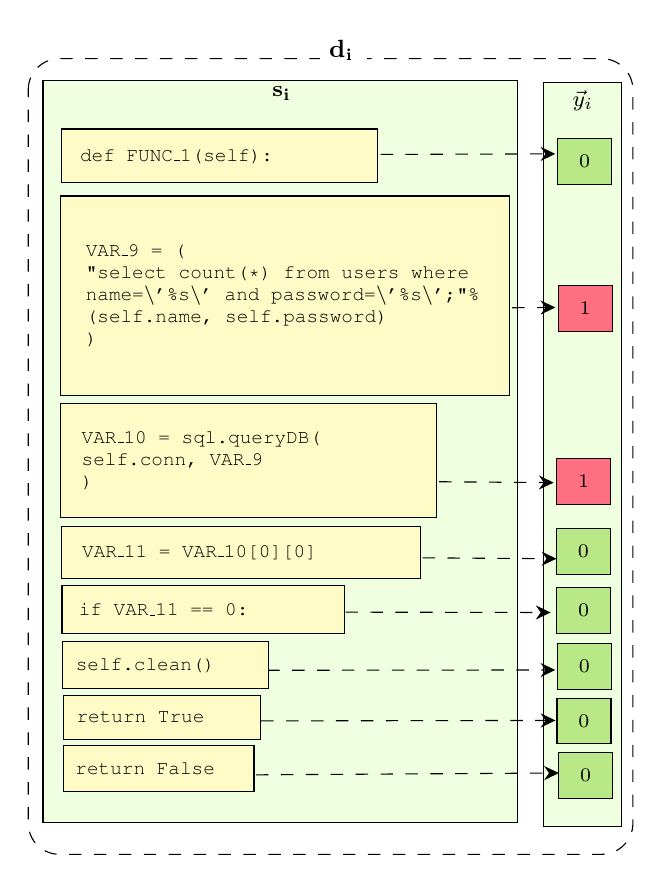
\begin{tikzpicture}[x=0.75pt,y=0.75pt,yscale=-1,xscale=1]
%uncomment if require: \path (0,413); %set diagram left start at 0, and has height of 413

%Shape: Rectangle [id:dp5178477671322261] 
\draw  [fill={rgb, 255:red, 239; green, 255; blue, 224 }  ,fill opacity=1 ] (449.13,24.67) -- (486.58,24.67) -- (486.58,383.33) -- (449.13,383.33) -- cycle ;
%Shape: Rectangle [id:dp12894625454637976] 
\draw  [fill={rgb, 255:red, 239; green, 255; blue, 224 }  ,fill opacity=1 ] (207.77,23.67) -- (436.25,23.67) -- (436.25,381.5) -- (207.77,381.5) -- cycle ;
%Straight Lines [id:da6258442396381019] 
\draw  [dash pattern={on 4.5pt off 4.5pt}]  (370.43,59.47) -- (451.6,59.21) ;
\draw [shift={(454.6,59.2)}, rotate = 179.82] [fill={rgb, 255:red, 0; green, 0; blue, 0 }  ][line width=0.08]  [draw opacity=0] (7.14,-3.43) -- (0,0) -- (7.14,3.43) -- (4.74,0) -- cycle    ;
%Straight Lines [id:da520135983630521] 
\draw  [dash pattern={on 4.5pt off 4.5pt}]  (433.81,133.33) -- (451.6,133.22) ;
\draw [shift={(454.6,133.2)}, rotate = 179.63] [fill={rgb, 255:red, 0; green, 0; blue, 0 }  ][line width=0.08]  [draw opacity=0] (7.14,-3.43) -- (0,0) -- (7.14,3.43) -- (4.74,0) -- cycle    ;
%Straight Lines [id:da7621693394483864] 
\draw  [dash pattern={on 4.5pt off 4.5pt}]  (310.4,358.39) -- (453.33,357.52) ;
\draw [shift={(456.33,357.5)}, rotate = 179.65] [fill={rgb, 255:red, 0; green, 0; blue, 0 }  ][line width=0.08]  [draw opacity=0] (7.14,-3.43) -- (0,0) -- (7.14,3.43) -- (4.74,0) -- cycle    ;
%Straight Lines [id:da0562112340178782] 
\draw  [dash pattern={on 4.5pt off 4.5pt}]  (390.67,253.83) -- (452.13,254.25) ;
\draw [shift={(455.13,254.27)}, rotate = 180.39] [fill={rgb, 255:red, 0; green, 0; blue, 0 }  ][line width=0.08]  [draw opacity=0] (7.14,-3.43) -- (0,0) -- (7.14,3.43) -- (4.74,0) -- cycle    ;
%Straight Lines [id:da07585087742541297] 
\draw  [dash pattern={on 4.5pt off 4.5pt}]  (353.53,280) -- (449.33,280.16) ;
\draw [shift={(452.33,280.17)}, rotate = 180.1] [fill={rgb, 255:red, 0; green, 0; blue, 0 }  ][line width=0.08]  [draw opacity=0] (7.14,-3.43) -- (0,0) -- (7.14,3.43) -- (4.74,0) -- cycle    ;
%Straight Lines [id:da8945437161769698] 
\draw  [dash pattern={on 4.5pt off 4.5pt}]  (315.84,308) -- (451.6,307.87) ;
\draw [shift={(454.6,307.87)}, rotate = 179.94] [fill={rgb, 255:red, 0; green, 0; blue, 0 }  ][line width=0.08]  [draw opacity=0] (7.14,-3.43) -- (0,0) -- (7.14,3.43) -- (4.74,0) -- cycle    ;
%Straight Lines [id:da8421526195500562] 
\draw  [dash pattern={on 4.5pt off 4.5pt}]  (312.93,332.4) -- (451.67,332.17) ;
\draw [shift={(454.67,332.17)}, rotate = 179.9] [fill={rgb, 255:red, 0; green, 0; blue, 0 }  ][line width=0.08]  [draw opacity=0] (7.14,-3.43) -- (0,0) -- (7.14,3.43) -- (4.74,0) -- cycle    ;
%Straight Lines [id:da28861365975593056] 
\draw  [dash pattern={on 4.5pt off 4.5pt}]  (398.67,217.17) -- (450.8,217.58) ;
\draw [shift={(453.8,217.6)}, rotate = 180.45] [fill={rgb, 255:red, 0; green, 0; blue, 0 }  ][line width=0.08]  [draw opacity=0] (7.14,-3.43) -- (0,0) -- (7.14,3.43) -- (4.74,0) -- cycle    ;
%Shape: Rectangle [id:dp20048853091704677] 
\draw  [dash pattern={on 4.5pt off 4.5pt}] (200.67,28.33) .. controls (200.67,20.05) and (207.38,13.33) .. (215.67,13.33) -- (477,13.33) .. controls (485.28,13.33) and (492,20.05) .. (492,28.33) -- (492,381.67) .. controls (492,389.95) and (485.28,396.67) .. (477,396.67) -- (215.67,396.67) .. controls (207.38,396.67) and (200.67,389.95) .. (200.67,381.67) -- cycle ;

% Text Node
\draw  [fill={rgb, 255:red, 255; green, 251; blue, 198 }  ,fill opacity=1 ]  (216.73,47.21) -- (368.73,47.21) -- (368.73,73.21) -- (216.73,73.21) -- cycle  ;
\draw (292.73,60.21) node  [font=\scriptsize] [align=left] {\begin{minipage}[lt]{100.63pt}\setlength\topsep{0pt}
{\fontfamily{pcr}\selectfont def FUNC\_1(self):}
\end{minipage}};
% Text Node
\draw  [fill={rgb, 255:red, 255; green, 251; blue, 198 }  ,fill opacity=1 ]  (216.42,79.51) -- (432.42,79.51) -- (432.42,175.51) -- (216.42,175.51) -- cycle  ;
\draw (324.42,127.51) node  [font=\scriptsize] [align=left] {\begin{minipage}[lt]{144.05pt}\setlength\topsep{0pt}
{\fontfamily{pcr}\selectfont VAR\_9 = ( \ \ }\\{\fontfamily{pcr}\selectfont  \ "select count(*) from users where 		name=\textbackslash '\%s\textbackslash ' and password=\textbackslash '\%s\textbackslash ';"\% (self.name, self.password)}\\{\fontfamily{pcr}\selectfont )}
\end{minipage}};
% Text Node
\draw  [fill={rgb, 255:red, 255; green, 251; blue, 198 }  ,fill opacity=1 ]  (216.29,179.35) -- (397.29,179.35) -- (397.29,234.35) -- (216.29,234.35) -- cycle  ;
\draw (306.79,206.85) node  [font=\scriptsize] [align=left] {\begin{minipage}[lt]{120.52pt}\setlength\topsep{0pt}
{\fontfamily{pcr}\selectfont VAR\_10 = sql.queryDB(}\\{\fontfamily{pcr}\selectfont self.conn, VAR\_9}\\{\fontfamily{pcr}\selectfont )}
\end{minipage}};
% Text Node
\draw  [fill={rgb, 255:red, 255; green, 251; blue, 198 }  ,fill opacity=1 ]  (216.79,238.69) -- (389.79,238.69) -- (389.79,263.69) -- (216.79,263.69) -- cycle  ;
\draw (303.29,251.19) node  [font=\scriptsize] [align=left] {\begin{minipage}[lt]{114.95pt}\setlength\topsep{0pt}
{\fontfamily{pcr}\selectfont VAR\_11 = VAR\_10[0][0]}
\end{minipage}};
% Text Node
\draw  [fill={rgb, 255:red, 255; green, 251; blue, 198 }  ,fill opacity=1 ]  (216.96,267.2) -- (352.96,267.2) -- (352.96,290.2) -- (216.96,290.2) -- cycle  ;
\draw (284.96,278.7) node  [font=\scriptsize] [align=left] {\begin{minipage}[lt]{89.9pt}\setlength\topsep{0pt}
{\fontfamily{pcr}\selectfont  if VAR\_11 == 0:}
\end{minipage}};
% Text Node
\draw  [fill={rgb, 255:red, 255; green, 251; blue, 198 }  ,fill opacity=1 ]  (217.35,293.97) -- (316.35,293.97) -- (316.35,316.97) -- (217.35,316.97) -- cycle  ;
\draw (266.85,305.47) node  [font=\scriptsize] [align=left] {\begin{minipage}[lt]{64.86pt}\setlength\topsep{0pt}
{\fontfamily{pcr}\selectfont  self.clean()}
\end{minipage}};
% Text Node
\draw  [fill={rgb, 255:red, 255; green, 251; blue, 198 }  ,fill opacity=1 ]  (217.46,344.33) -- (309.46,344.33) -- (309.46,366.33) -- (217.46,366.33) -- cycle  ;
\draw (263.46,355.33) node  [font=\scriptsize] [align=left] {\begin{minipage}[lt]{60.06pt}\setlength\topsep{0pt}
{\fontfamily{pcr}\selectfont return False}
\end{minipage}};
% Text Node
\draw  [fill={rgb, 255:red, 255; green, 251; blue, 198 }  ,fill opacity=1 ]  (217.56,320.17) -- (312.56,320.17) -- (312.56,341.17) -- (217.56,341.17) -- cycle  ;
\draw (265.06,330.67) node  [font=\scriptsize] [align=left] {\begin{minipage}[lt]{61.66pt}\setlength\topsep{0pt}
{\fontfamily{pcr}\selectfont return True}
\end{minipage}};
% Text Node
\draw  [fill={rgb, 255:red, 184; green, 233; blue, 134 }  ,fill opacity=1 ]  (455.76,51.97) -- (481.76,51.97) -- (481.76,73.97) -- (455.76,73.97) -- cycle  ;
\draw (468.76,62.97) node  [font=\scriptsize] [align=left] {\begin{minipage}[lt]{15.08pt}\setlength\topsep{0pt}
\begin{center}
0
\end{center}

\end{minipage}};
% Text Node
\draw  [fill={rgb, 255:red, 255; green, 111; blue, 130 }  ,fill opacity=1 ]  (456,122.63) -- (482,122.63) -- (482,144.63) -- (456,144.63) -- cycle  ;
\draw (469,133.63) node  [font=\scriptsize] [align=left] {\begin{minipage}[lt]{15.08pt}\setlength\topsep{0pt}
\begin{center}
1
\end{center}

\end{minipage}};
% Text Node
\draw  [fill={rgb, 255:red, 184; green, 233; blue, 134 }  ,fill opacity=1 ]  (455.1,239.8) -- (481.1,239.8) -- (481.1,261.8) -- (455.1,261.8) -- cycle  ;
\draw (468.1,250.8) node  [font=\scriptsize] [align=left] {\begin{minipage}[lt]{15.08pt}\setlength\topsep{0pt}
\begin{center}
0
\end{center}

\end{minipage}};
% Text Node
\draw  [fill={rgb, 255:red, 184; green, 233; blue, 134 }  ,fill opacity=1 ]  (455.29,268.3) -- (481.29,268.3) -- (481.29,290.3) -- (455.29,290.3) -- cycle  ;
\draw (468.29,279.3) node  [font=\scriptsize] [align=left] {\begin{minipage}[lt]{15.08pt}\setlength\topsep{0pt}
\begin{center}
0
\end{center}

\end{minipage}};
% Text Node
\draw  [fill={rgb, 255:red, 184; green, 233; blue, 134 }  ,fill opacity=1 ]  (455.59,295.17) -- (481.59,295.17) -- (481.59,317.17) -- (455.59,317.17) -- cycle  ;
\draw (468.59,306.17) node  [font=\scriptsize] [align=left] {\begin{minipage}[lt]{15.08pt}\setlength\topsep{0pt}
\begin{center}
0
\end{center}

\end{minipage}};
% Text Node
\draw  [fill={rgb, 255:red, 184; green, 233; blue, 134 }  ,fill opacity=1 ]  (455.43,321.47) -- (481.43,321.47) -- (481.43,343.47) -- (455.43,343.47) -- cycle  ;
\draw (468.43,332.47) node  [font=\scriptsize] [align=left] {\begin{minipage}[lt]{15.08pt}\setlength\topsep{0pt}
\begin{center}
0
\end{center}

\end{minipage}};
% Text Node
\draw  [fill={rgb, 255:red, 184; green, 233; blue, 134 }  ,fill opacity=1 ]  (456.24,347.57) -- (482.24,347.57) -- (482.24,369.57) -- (456.24,369.57) -- cycle  ;
\draw (469.24,358.57) node  [font=\scriptsize] [align=left] {\begin{minipage}[lt]{15.08pt}\setlength\topsep{0pt}
\begin{center}
0
\end{center}

\end{minipage}};
% Text Node
\draw  [fill={rgb, 255:red, 255; green, 111; blue, 130 }  ,fill opacity=1 ]  (455.29,206.13) -- (481.29,206.13) -- (481.29,228.13) -- (455.29,228.13) -- cycle  ;
\draw (468.29,217.13) node  [font=\scriptsize] [align=left] {\begin{minipage}[lt]{15.08pt}\setlength\topsep{0pt}
\begin{center}
1
\end{center}

\end{minipage}};
% Text Node
\draw  [color={rgb, 255:red, 255; green, 255; blue, 255 }  ,draw opacity=1 ][fill={rgb, 255:red, 255; green, 255; blue, 255 }  ,fill opacity=1 ]  (341.43,-1.33) -- (363.43,-1.33) -- (363.43,22.67) -- (341.43,22.67) -- cycle  ;
\draw (344.43,3.07) node [anchor=north west][inner sep=0.75pt]  [font=\small]  {$\mathbf{d_{i}}$};
% Text Node
\draw (317.02,25.4) node [anchor=north west][inner sep=0.75pt]  [font=\footnotesize]  {$\mathbf{s_{i}}$};
% Text Node
\draw (461.73,27.4) node [anchor=north west][inner sep=0.75pt]  [font=\footnotesize]  {$\Vec{y}_{i}$};


\end{tikzpicture}
    \caption{An illustration of a  function gadget $\mathbf{d_i} \in \mathbf{D}$ that consists of 8 statements $s_{ij} \in \mathbf{s}_i$ and their corresponding labels $y_{ij} \in \Vec{y}_i$. All statements have had their trailing spaces, tab, and newline escape removed. Here, two of the statements, namely $s_{i2}$, and $s_{i3}$, are susceptible to SQL injection attacks. An attacker can exploit this vulnerability by manipulating the input parameters `self.name` and `self.password` to insert malicious SQL code into the query.
} \label{fig:func_gadget}
\end{figure}

In this paper, the classification of vulnerable statements is treated as a multi-class problem. Given a source file, all statements are extracted and grouped into function gadgets, where each gadget represents a set of statements that belong to a single function. Our dataset can be denoted as $\mathbf{D=\{\mathbf{d_1, d_2, .., d_N}}\}$, where N is the number of gadgets. Let $\mathbf{s_i}$ and $\vec{y_i}$ represent the set of statements of function gadget $\mathbf{d_i}$ and their corresponding labels, we have  $\mathbf{d_i}=(\mathbf{s_i}, \Vec{y_i})=((s_{ij},y_{ij})|s_{ij}\in \mathbf{s_i}, y_{ij} \in \Vec{y_i}, y_{ij}\in\{0,1,2,.., c-1\}, j \in\{1,2,..,n\})$, in which $c$ denotes the number of classes and $n$ is the number of statements in the function gadget. In figure \ref{fig:func_gadget}, a function gadget $\mathbf{d_i}$ is depicted, wherein each statement $s_{ij}$ is a piece of text with all trailing spaces, tabs, and newline breaks removed. The statements in $\mathbf{s_i}$ are arranged in the same order as they appear in the original function from which they were extracted. The vector $\Vec{y}_i$ contains the labels $y_{ij}$ that are corresponding to each statement $s_{ij}$.

    
Let $f$ and $\theta$ be the deep-learning model and the trainable weights that are used to map $\mathbf{s_i} \rightarrow \Vec{y_i}$, we have  $\hat{Y}_i=f(\mathbf{s_i},\mathbf{\theta})$, where $\hat{Y}_i \in \mathbb{R}^{n\times c}$ is a matrix that denotes predicted probability distributions of each label for all statements in $\mathbf{s_i}$. Our final goal is to find the set of weights $\theta^*$ that can help  approximate $\hat{Y}_i$ to $\Vec{y_i}$ by minimizing a loss function $L(\theta)$, the whole learning process can be formulated as:
\begin{equation} \label{equa:problem_formation}
\argmin_\theta L(\theta)=\sum _{i=1}^{N}\sum_{j=1}^{n}\frac{l_{ij}(f(s_{ij},\mathbf{\theta}),y_{ij})}{\sum _{i=1}^{n} w_{y_{ij}}}\end{equation}
 
Here in equation \ref{equa:problem_formation}, $l_{ij}$ denotes the weighted cross-entropy (WCE) loss function, and $w_{y_{ij}}$ is the weight assigned to each sample based on its ground truth label.

\section{Methodology} \label{sec:method}
This section discussed details of the pipeline used for our approach including phases for data preprocessing, training, and inference. 
\begin{figure*}[h]
    \centering
    

\tikzset{every picture/.style={line width=0.75pt}} %set default line width to 0.75pt        

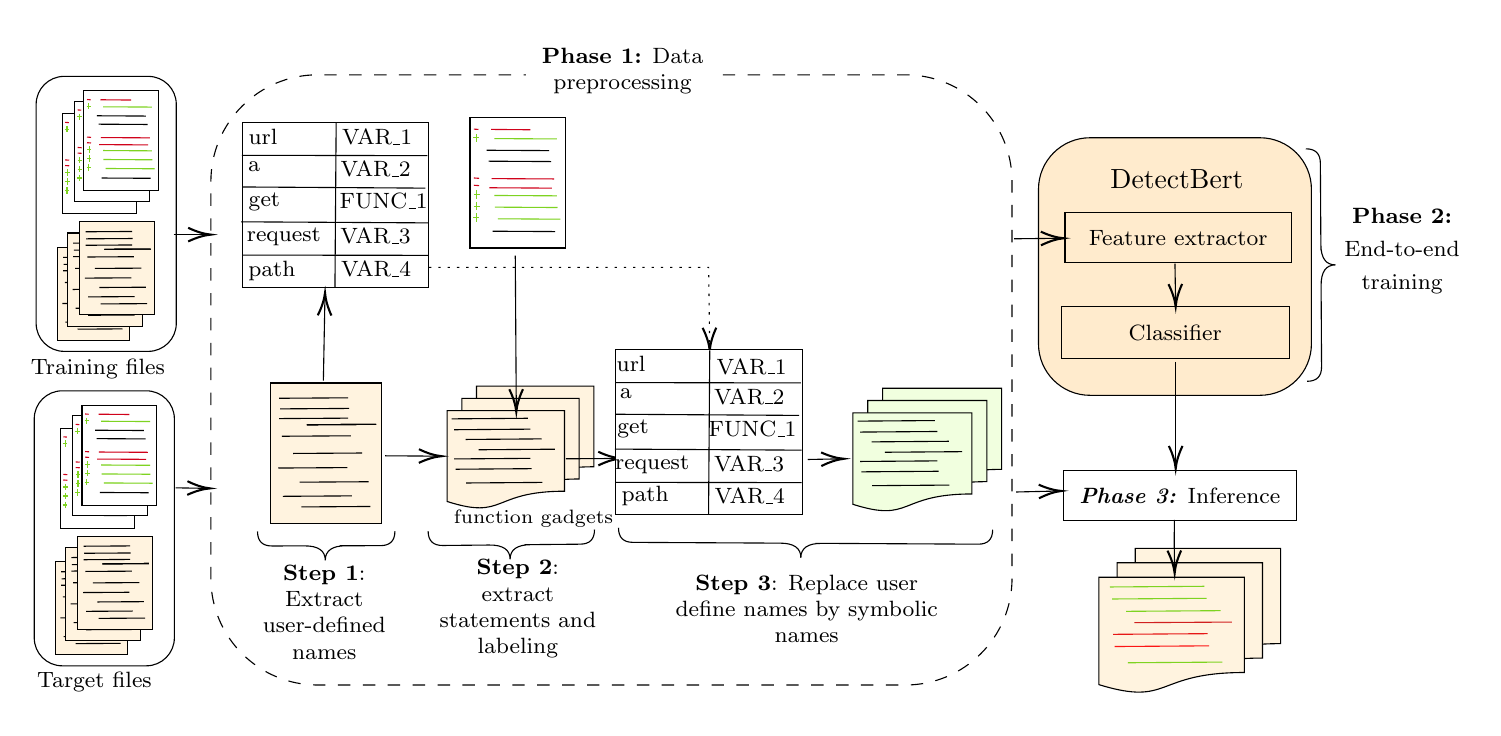
\begin{tikzpicture}[x=0.75pt,y=0.75pt,yscale=-1,xscale=1]
%uncomment if require: \path (0,313); %set diagram left start at 0, and has height of 313

%Rounded Rect [id:dp5407352618857819] 
\draw  [fill={rgb, 255:red, 255; green, 235; blue, 205 }  ,fill opacity=1 ] (488.67,67.87) .. controls (488.67,54.16) and (499.78,43.05) .. (513.48,43.05) -- (595.35,43.05) .. controls (609.06,43.05) and (620.17,54.16) .. (620.17,67.87) -- (620.17,142.32) .. controls (620.17,156.02) and (609.06,167.14) .. (595.35,167.14) -- (513.48,167.14) .. controls (499.78,167.14) and (488.67,156.02) .. (488.67,142.32) -- cycle ;
%Flowchart: Multidocument [id:dp03948637433927171] 
\draw  [color={rgb, 255:red, 0; green, 0; blue, 0 }  ,draw opacity=1 ][fill={rgb, 255:red, 255; green, 243; blue, 223 }  ,fill opacity=1 ] (217.89,162.72) -- (274.43,162.72) -- (274.43,201.57) .. controls (239.1,201.57) and (246.16,215.59) .. (217.89,206.52) -- cycle ; \draw  [color={rgb, 255:red, 0; green, 0; blue, 0 }  ,draw opacity=1 ][fill={rgb, 255:red, 255; green, 243; blue, 223 }  ,fill opacity=1 ] (210.83,168.61) -- (267.37,168.61) -- (267.37,207.46) .. controls (232.03,207.46) and (239.1,221.47) .. (210.83,212.41) -- cycle ; \draw  [color={rgb, 255:red, 0; green, 0; blue, 0 }  ,draw opacity=1 ][fill={rgb, 255:red, 255; green, 243; blue, 223 }  ,fill opacity=1 ] (203.76,174.49) -- (260.3,174.49) -- (260.3,213.35) .. controls (224.96,213.35) and (232.03,227.36) .. (203.76,218.29) -- cycle ;
%Straight Lines [id:da9944346698756492] 
\draw [color={rgb, 255:red, 0; green, 0; blue, 0 }  ,draw opacity=1 ][fill={rgb, 255:red, 255; green, 243; blue, 223 }  ,fill opacity=1 ]   (205.97,178.48) -- (242.69,178.2) ;
%Straight Lines [id:da990779165722957] 
\draw [color={rgb, 255:red, 0; green, 0; blue, 0 }  ,draw opacity=1 ][fill={rgb, 255:red, 255; green, 243; blue, 223 }  ,fill opacity=1 ]   (218.97,193.37) -- (255.69,193.1) ;
%Straight Lines [id:da7504058793027286] 
\draw [color={rgb, 255:red, 0; green, 0; blue, 0 }  ,draw opacity=1 ][fill={rgb, 255:red, 255; green, 243; blue, 223 }  ,fill opacity=1 ]   (207.18,183.72) -- (243.9,183.44) ;
%Straight Lines [id:da5634896373265414] 
\draw [color={rgb, 255:red, 0; green, 0; blue, 0 }  ,draw opacity=1 ][fill={rgb, 255:red, 255; green, 243; blue, 223 }  ,fill opacity=1 ]   (207.18,197.79) -- (243.9,197.51) ;
%Straight Lines [id:da7162822368630877] 
\draw [color={rgb, 255:red, 0; green, 0; blue, 0 }  ,draw opacity=1 ][fill={rgb, 255:red, 255; green, 243; blue, 223 }  ,fill opacity=1 ]   (212.62,188.41) -- (249.34,188.13) ;
%Straight Lines [id:da5699700969107819] 
\draw [color={rgb, 255:red, 0; green, 0; blue, 0 }  ,draw opacity=1 ][fill={rgb, 255:red, 255; green, 243; blue, 223 }  ,fill opacity=1 ]   (207.79,202.75) -- (244.51,202.48) ;
%Straight Lines [id:da06367411789537192] 
\draw [color={rgb, 255:red, 0; green, 0; blue, 0 }  ,draw opacity=1 ][fill={rgb, 255:red, 255; green, 243; blue, 223 }  ,fill opacity=1 ]   (212.92,209.38) -- (249.64,209.1) ;

%Straight Lines [id:da979947140929379] 
\draw    (144.13,160.1) -- (144.89,119.72) ;
\draw [shift={(144.93,117.72)}, rotate = 91.08] [color={rgb, 255:red, 0; green, 0; blue, 0 }  ][line width=0.75]    (10.93,-3.29) .. controls (6.95,-1.4) and (3.31,-0.3) .. (0,0) .. controls (3.31,0.3) and (6.95,1.4) .. (10.93,3.29)   ;
%Flowchart: Process [id:dp08889225830773517] 
\draw  [fill={rgb, 255:red, 255; green, 243; blue, 223 }  ,fill opacity=1 ] (118.59,161.22) -- (172.17,161.22) -- (172.17,228.89) -- (118.59,228.89) -- cycle ;
%Straight Lines [id:da5795634366087907] 
\draw [fill={rgb, 255:red, 255; green, 243; blue, 223 }  ,fill opacity=1 ]   (122.83,168.56) -- (138.69,168.46) -- (156.09,168.35) ;
%Straight Lines [id:da037406032462627525] 
\draw [fill={rgb, 255:red, 255; green, 243; blue, 223 }  ,fill opacity=1 ]   (123.28,173.67) -- (139.13,173.57) -- (156.54,173.45) ;
%Straight Lines [id:da31933329088980567] 
\draw [fill={rgb, 255:red, 255; green, 243; blue, 223 }  ,fill opacity=1 ]   (122.83,178.35) -- (138.69,178.25) -- (156.09,178.14) ;
%Straight Lines [id:da9730748688887287] 
\draw [fill={rgb, 255:red, 255; green, 243; blue, 223 }  ,fill opacity=1 ]   (124.17,186.86) -- (140.03,186.76) -- (157.43,186.65) ;
%Straight Lines [id:da47479067052888313] 
\draw [fill={rgb, 255:red, 255; green, 243; blue, 223 }  ,fill opacity=1 ]   (136.23,181.33) -- (152.08,181.23) -- (169.49,181.11) ;
%Straight Lines [id:da4143023391361096] 
\draw [fill={rgb, 255:red, 255; green, 243; blue, 223 }  ,fill opacity=1 ]   (136.23,181.33) -- (152.08,181.23) -- (169.49,181.11) ;
%Straight Lines [id:da4818870317406938] 
\draw [fill={rgb, 255:red, 255; green, 243; blue, 223 }  ,fill opacity=1 ]   (129.53,195.15) -- (145.38,195.05) -- (162.79,194.94) ;
%Straight Lines [id:da5811373617437334] 
\draw [fill={rgb, 255:red, 255; green, 243; blue, 223 }  ,fill opacity=1 ]   (136.23,181.33) -- (152.08,181.23) -- (169.49,181.11) ;
%Straight Lines [id:da8075525914940331] 
\draw [fill={rgb, 255:red, 255; green, 243; blue, 223 }  ,fill opacity=1 ]   (122.39,202.18) -- (138.24,202.08) -- (155.65,201.97) ;
%Straight Lines [id:da9083084701422104] 
\draw [fill={rgb, 255:red, 255; green, 243; blue, 223 }  ,fill opacity=1 ]   (132.66,208.99) -- (148.51,208.89) -- (165.92,208.78) ;
%Straight Lines [id:da5974790746282925] 
\draw [fill={rgb, 255:red, 255; green, 243; blue, 223 }  ,fill opacity=1 ]   (124.62,215.8) -- (140.47,215.7) -- (157.88,215.59) ;
%Straight Lines [id:da5447010970733284] 
\draw [fill={rgb, 255:red, 255; green, 243; blue, 223 }  ,fill opacity=1 ]   (133.55,220.91) -- (149.4,220.81) -- (166.81,220.69) ;

%Straight Lines [id:da3732122853030273] 
\draw  [dash pattern={on 0.84pt off 2.51pt}]  (195.08,105.47) -- (329.77,105.47) -- (330.26,143.53) ;
\draw [shift={(330.29,145.53)}, rotate = 269.25] [color={rgb, 255:red, 0; green, 0; blue, 0 }  ][line width=0.75]    (10.93,-3.29) .. controls (6.95,-1.4) and (3.31,-0.3) .. (0,0) .. controls (3.31,0.3) and (6.95,1.4) .. (10.93,3.29)   ;
%Straight Lines [id:da2759559394676936] 
\draw    (173.91,196.28) -- (199.08,196.45) ;
\draw [shift={(201.08,196.47)}, rotate = 180.41] [color={rgb, 255:red, 0; green, 0; blue, 0 }  ][line width=0.75]    (10.93,-3.29) .. controls (6.95,-1.4) and (3.31,-0.3) .. (0,0) .. controls (3.31,0.3) and (6.95,1.4) .. (10.93,3.29)   ;
%Shape: Brace [id:dp9516034027102489] 
\draw   (112.4,232.75) .. controls (112.41,237.42) and (114.75,239.74) .. (119.42,239.73) -- (135.03,239.68) .. controls (141.7,239.66) and (145.04,241.98) .. (145.05,246.65) .. controls (145.04,241.98) and (148.36,239.64) .. (155.03,239.62)(152.03,239.63) -- (171.61,239.57) .. controls (176.28,239.56) and (178.6,237.22) .. (178.59,232.55) ;
%Shape: Brace [id:dp0005650171589655084] 
\draw   (194.59,232.55) .. controls (194.64,237.22) and (196.99,239.53) .. (201.66,239.49) -- (224.04,239.27) .. controls (230.71,239.21) and (234.06,241.51) .. (234.1,246.18) .. controls (234.06,241.51) and (237.37,239.15) .. (244.04,239.09)(241.04,239.11) -- (267.82,238.86) .. controls (272.49,238.82) and (274.8,236.47) .. (274.75,231.8) ;
%Shape: Brace [id:dp39161724968333744] 
\draw   (286.33,230.96) .. controls (286.31,235.63) and (288.63,237.97) .. (293.3,237.99) -- (364.21,238.36) .. controls (370.88,238.4) and (374.2,240.75) .. (374.17,245.42) .. controls (374.2,240.75) and (377.54,238.44) .. (384.21,238.47)(381.21,238.45) -- (459.56,238.86) .. controls (464.23,238.89) and (466.57,236.57) .. (466.59,231.9) ;
%Straight Lines [id:da8897877371292919] 
\draw    (260.93,197.72) -- (285.52,197.57) ;
\draw [shift={(287.52,197.55)}, rotate = 179.64] [color={rgb, 255:red, 0; green, 0; blue, 0 }  ][line width=0.75]    (10.93,-3.29) .. controls (6.95,-1.4) and (3.31,-0.3) .. (0,0) .. controls (3.31,0.3) and (6.95,1.4) .. (10.93,3.29)   ;
%Straight Lines [id:da38586209961748397] 
\draw    (377.5,198.06) -- (392.93,197.76) ;
\draw [shift={(394.93,197.72)}, rotate = 178.88] [color={rgb, 255:red, 0; green, 0; blue, 0 }  ][line width=0.75]    (10.93,-3.29) .. controls (6.95,-1.4) and (3.31,-0.3) .. (0,0) .. controls (3.31,0.3) and (6.95,1.4) .. (10.93,3.29)   ;
%Flowchart: Alternative Process [id:dp9304959099868064] 
\draw  [dash pattern={on 4.5pt off 4.5pt}] (89.93,64.17) .. controls (89.93,35.75) and (112.97,12.72) .. (141.38,12.72) -- (424.48,12.72) .. controls (452.9,12.72) and (475.93,35.75) .. (475.93,64.17) -- (475.93,255.27) .. controls (475.93,283.68) and (452.9,306.72) .. (424.48,306.72) -- (141.38,306.72) .. controls (112.97,306.72) and (89.93,283.68) .. (89.93,255.27) -- cycle ;
%Flowchart: Multidocument [id:dp05796369385915745] 
\draw  [fill={rgb, 255:red, 241; green, 255; blue, 223 }  ,fill opacity=1 ] (413.59,163.72) -- (470.93,163.72) -- (470.93,202.82) .. controls (435.1,202.82) and (442.26,216.92) .. (413.59,207.8) -- cycle ; \draw  [fill={rgb, 255:red, 241; green, 255; blue, 223 }  ,fill opacity=1 ] (406.43,169.64) -- (463.77,169.64) -- (463.77,208.74) .. controls (427.93,208.74) and (435.1,222.85) .. (406.43,213.72) -- cycle ; \draw  [fill={rgb, 255:red, 241; green, 255; blue, 223 }  ,fill opacity=1 ] (399.26,175.57) -- (456.6,175.57) -- (456.6,214.67) .. controls (420.76,214.67) and (427.93,228.77) .. (399.26,219.65) -- cycle ;
%Straight Lines [id:da45589121987746695] 
\draw [fill={rgb, 255:red, 241; green, 255; blue, 223 }  ,fill opacity=1 ]   (401.5,179.58) -- (438.74,179.3) ;
%Straight Lines [id:da8972012548715187] 
\draw [fill={rgb, 255:red, 241; green, 255; blue, 223 }  ,fill opacity=1 ]   (414.68,194.57) -- (451.92,194.29) ;
%Straight Lines [id:da3781586819477176] 
\draw [fill={rgb, 255:red, 241; green, 255; blue, 223 }  ,fill opacity=1 ]   (402.73,184.85) -- (439.97,184.57) ;
%Straight Lines [id:da7030947462767194] 
\draw [fill={rgb, 255:red, 241; green, 255; blue, 223 }  ,fill opacity=1 ]   (402.73,199.01) -- (439.97,198.73) ;
%Straight Lines [id:da3133605136700426] 
\draw [fill={rgb, 255:red, 241; green, 255; blue, 223 }  ,fill opacity=1 ]   (408.25,189.57) -- (445.49,189.29) ;
%Straight Lines [id:da915070418974427] 
\draw [fill={rgb, 255:red, 241; green, 255; blue, 223 }  ,fill opacity=1 ]   (403.34,204.01) -- (440.58,203.73) ;
%Straight Lines [id:da8506148325901877] 
\draw [fill={rgb, 255:red, 241; green, 255; blue, 223 }  ,fill opacity=1 ]   (408.55,210.67) -- (445.79,210.39) ;

%Straight Lines [id:da9067026636271347] 
\draw    (236.59,99.89) -- (237.07,173.14) ;
\draw [shift={(237.08,175.14)}, rotate = 269.63] [color={rgb, 255:red, 0; green, 0; blue, 0 }  ][line width=0.75]    (10.93,-3.29) .. controls (6.95,-1.4) and (3.31,-0.3) .. (0,0) .. controls (3.31,0.3) and (6.95,1.4) .. (10.93,3.29)   ;
%Flowchart: Process [id:dp15158939778845038] 
\draw  [fill={rgb, 255:red, 255; green, 255; blue, 255 }  ,fill opacity=1 ] (285.07,145.22) -- (374.93,145.22) -- (374.93,224.69) -- (285.07,224.69) -- cycle ;
%Straight Lines [id:da4361526525843711] 
\draw [fill={rgb, 255:red, 255; green, 255; blue, 255 }  ,fill opacity=1 ]   (330.29,145.53) -- (329.71,224.37) ;
%Straight Lines [id:da7392899934986592] 
\draw [fill={rgb, 255:red, 255; green, 255; blue, 255 }  ,fill opacity=1 ]   (284.85,161.01) -- (374.24,161.17) ;
%Straight Lines [id:da3211677674513349] 
\draw [fill={rgb, 255:red, 255; green, 255; blue, 255 }  ,fill opacity=1 ]   (285.17,176.26) -- (373.33,176.82) ;
%Straight Lines [id:da8922901205210203] 
\draw [fill={rgb, 255:red, 255; green, 255; blue, 255 }  ,fill opacity=1 ]   (284.52,193.05) -- (374.5,193.56) ;
%Straight Lines [id:da8901957672617915] 
\draw [fill={rgb, 255:red, 255; green, 255; blue, 255 }  ,fill opacity=1 ]   (285.07,209.08) -- (374.5,209.2) ;
%Straight Lines [id:da365148841633435] 
\draw    (554.42,103.64) -- (554.73,122.47) ;
\draw [shift={(554.77,124.47)}, rotate = 269.04] [color={rgb, 255:red, 0; green, 0; blue, 0 }  ][line width=0.75]    (10.93,-3.29) .. controls (6.95,-1.4) and (3.31,-0.3) .. (0,0) .. controls (3.31,0.3) and (6.95,1.4) .. (10.93,3.29)   ;
%Flowchart: Multidocument [id:dp6590713783006148] 
\draw  [fill={rgb, 255:red, 255; green, 243; blue, 223 }  ,fill opacity=1 ] (535.28,240.86) -- (605.36,240.86) -- (605.36,286.78) .. controls (561.56,286.78) and (570.32,303.33) .. (535.28,292.62) -- cycle ; \draw  [fill={rgb, 255:red, 255; green, 243; blue, 223 }  ,fill opacity=1 ] (526.52,247.82) -- (596.6,247.82) -- (596.6,293.73) .. controls (552.8,293.73) and (561.56,310.29) .. (526.52,299.58) -- cycle ; \draw  [fill={rgb, 255:red, 255; green, 243; blue, 223 }  ,fill opacity=1 ] (517.76,254.77) -- (587.84,254.77) -- (587.84,300.69) .. controls (544.04,300.69) and (552.8,317.25) .. (517.76,306.53) -- cycle ;
%Straight Lines [id:da41449888213867725] 
\draw [color={rgb, 255:red, 126; green, 211; blue, 33 }  ,draw opacity=1 ][fill={rgb, 255:red, 255; green, 243; blue, 223 }  ,fill opacity=1 ]   (523.12,259.48) -- (568.63,259.15) ;
%Straight Lines [id:da08648834587080123] 
\draw [color={rgb, 255:red, 208; green, 32; blue, 32 }  ,draw opacity=1 ][fill={rgb, 255:red, 255; green, 243; blue, 223 }  ,fill opacity=1 ]   (534.87,276.68) -- (581.83,276.39) ;
%Straight Lines [id:da5669302852382512] 
\draw [color={rgb, 255:red, 126; green, 211; blue, 33 }  ,draw opacity=1 ][fill={rgb, 255:red, 255; green, 243; blue, 223 }  ,fill opacity=1 ]   (524.18,265.27) -- (569.69,264.94) ;
%Straight Lines [id:da7093942401057922] 
\draw [color={rgb, 255:red, 230; green, 23; blue, 23 }  ,draw opacity=1 ][fill={rgb, 255:red, 255; green, 243; blue, 223 }  ,fill opacity=1 ]   (524.61,282.3) -- (553.94,282.09) -- (570.13,281.98) ;
%Straight Lines [id:da560257514861523] 
\draw [color={rgb, 255:red, 126; green, 211; blue, 33 }  ,draw opacity=1 ][fill={rgb, 255:red, 255; green, 243; blue, 223 }  ,fill opacity=1 ]   (530.92,271.22) -- (576.44,270.89) ;
%Straight Lines [id:da3555099228205638] 
\draw [color={rgb, 255:red, 252; green, 21; blue, 21 }  ,draw opacity=1 ][fill={rgb, 255:red, 255; green, 243; blue, 223 }  ,fill opacity=1 ]   (525.36,288.17) -- (562.66,287.9) -- (570.88,287.84) ;
%Straight Lines [id:da5926018077208339] 
\draw [color={rgb, 255:red, 126; green, 211; blue, 33 }  ,draw opacity=1 ][fill={rgb, 255:red, 255; green, 243; blue, 223 }  ,fill opacity=1 ]   (531.73,295.99) -- (577.25,295.67) ;

%Straight Lines [id:da29232905356292016] 
\draw    (554.15,227.18) -- (554.06,238.21) -- (554.24,250.89) ;
\draw [shift={(554.27,252.89)}, rotate = 269.18] [color={rgb, 255:red, 0; green, 0; blue, 0 }  ][line width=0.75]    (10.93,-3.29) .. controls (6.95,-1.4) and (3.31,-0.3) .. (0,0) .. controls (3.31,0.3) and (6.95,1.4) .. (10.93,3.29)   ;
%Straight Lines [id:da02000362343106299] 
\draw    (71.93,89.72) -- (87.93,89.72) ;
\draw [shift={(89.93,89.72)}, rotate = 180] [color={rgb, 255:red, 0; green, 0; blue, 0 }  ][line width=0.75]    (10.93,-3.29) .. controls (6.95,-1.4) and (3.31,-0.3) .. (0,0) .. controls (3.31,0.3) and (6.95,1.4) .. (10.93,3.29)   ;
%Straight Lines [id:da011734998220744197] 
\draw    (72.93,211.72) -- (87.53,211.95) ;
\draw [shift={(89.53,211.98)}, rotate = 180.91] [color={rgb, 255:red, 0; green, 0; blue, 0 }  ][line width=0.75]    (10.93,-3.29) .. controls (6.95,-1.4) and (3.31,-0.3) .. (0,0) .. controls (3.31,0.3) and (6.95,1.4) .. (10.93,3.29)   ;
%Straight Lines [id:da22536054238819458] 
\draw    (476.93,91.72) -- (498.77,91.49) ;
\draw [shift={(500.77,91.47)}, rotate = 179.4] [color={rgb, 255:red, 0; green, 0; blue, 0 }  ][line width=0.75]    (10.93,-3.29) .. controls (6.95,-1.4) and (3.31,-0.3) .. (0,0) .. controls (3.31,0.3) and (6.95,1.4) .. (10.93,3.29)   ;
%Straight Lines [id:da8078757470371325] 
\draw    (477.93,213.72) -- (497.77,213.26) ;
\draw [shift={(499.77,213.22)}, rotate = 178.69] [color={rgb, 255:red, 0; green, 0; blue, 0 }  ][line width=0.75]    (10.93,-3.29) .. controls (6.95,-1.4) and (3.31,-0.3) .. (0,0) .. controls (3.31,0.3) and (6.95,1.4) .. (10.93,3.29)   ;
%Flowchart: Process [id:dp3610014250983158] 
\draw   (105.07,35.72) -- (194.93,35.72) -- (194.93,115.19) -- (105.07,115.19) -- cycle ;
%Straight Lines [id:da665587812140966] 
\draw    (150.29,36.03) -- (149.71,114.87) ;
%Straight Lines [id:da3748714523363281] 
\draw    (104.85,51.51) -- (194.24,51.67) ;
%Straight Lines [id:da5324881662476957] 
\draw    (105.17,66.76) -- (193.33,67.32) ;
%Straight Lines [id:da3760317228247998] 
\draw    (104.52,83.55) -- (194.5,84.06) ;
%Straight Lines [id:da2731803273744109] 
\draw    (105.07,99.58) -- (194.5,99.7) ;

%Flowchart: Process [id:dp9473525968344061] 
\draw  [fill={rgb, 255:red, 255; green, 243; blue, 223 }  ,fill opacity=1 ] (15.93,95.82) -- (50.84,95.82) -- (50.84,140.55) -- (15.93,140.55) -- cycle ;
%Straight Lines [id:da041410534351406625] 
\draw [fill={rgb, 255:red, 255; green, 243; blue, 223 }  ,fill opacity=1 ]   (18.69,100.67) -- (29.02,100.61) -- (40.36,100.53) ;
%Straight Lines [id:da8655314620397554] 
\draw [fill={rgb, 255:red, 255; green, 243; blue, 223 }  ,fill opacity=1 ]   (18.98,104.05) -- (29.31,103.98) -- (40.66,103.91) ;
%Straight Lines [id:da9164589930296427] 
\draw [fill={rgb, 255:red, 255; green, 243; blue, 223 }  ,fill opacity=1 ]   (18.69,107.14) -- (29.02,107.08) -- (40.36,107) ;
%Straight Lines [id:da8208125704816798] 
\draw [fill={rgb, 255:red, 255; green, 243; blue, 223 }  ,fill opacity=1 ]   (19.56,112.77) -- (29.89,112.7) -- (41.24,112.63) ;
%Straight Lines [id:da7032688319245235] 
\draw [fill={rgb, 255:red, 255; green, 243; blue, 223 }  ,fill opacity=1 ]   (27.42,109.11) -- (37.75,109.04) -- (49.09,108.97) ;
%Straight Lines [id:da3728236227048398] 
\draw [fill={rgb, 255:red, 255; green, 243; blue, 223 }  ,fill opacity=1 ]   (27.42,109.11) -- (37.75,109.04) -- (49.09,108.97) ;
%Straight Lines [id:da7719823340173988] 
\draw [fill={rgb, 255:red, 255; green, 243; blue, 223 }  ,fill opacity=1 ]   (23.05,118.25) -- (33.38,118.18) -- (44.73,118.11) ;
%Straight Lines [id:da31504592786843144] 
\draw [fill={rgb, 255:red, 255; green, 243; blue, 223 }  ,fill opacity=1 ]   (27.42,109.11) -- (37.75,109.04) -- (49.09,108.97) ;
%Straight Lines [id:da31780919635958194] 
\draw [fill={rgb, 255:red, 255; green, 243; blue, 223 }  ,fill opacity=1 ]   (18.4,122.9) -- (28.73,122.83) -- (40.07,122.75) ;
%Straight Lines [id:da6660501563445367] 
\draw [fill={rgb, 255:red, 255; green, 243; blue, 223 }  ,fill opacity=1 ]   (25.09,127.4) -- (35.42,127.33) -- (46.76,127.26) ;
%Straight Lines [id:da9751001607981287] 
\draw [fill={rgb, 255:red, 255; green, 243; blue, 223 }  ,fill opacity=1 ]   (19.85,131.9) -- (30.18,131.83) -- (41.53,131.76) ;
%Straight Lines [id:da4811814017829523] 
\draw [fill={rgb, 255:red, 255; green, 243; blue, 223 }  ,fill opacity=1 ]   (25.67,135.27) -- (36,135.21) -- (47.35,135.13) ;

%Flowchart: Process [id:dp9892338170596406] 
\draw  [fill={rgb, 255:red, 255; green, 243; blue, 223 }  ,fill opacity=1 ] (20.73,88.94) -- (56.8,88.94) -- (56.8,133.88) -- (20.73,133.88) -- cycle ;
%Straight Lines [id:da28577536538298687] 
\draw [fill={rgb, 255:red, 255; green, 243; blue, 223 }  ,fill opacity=1 ]   (23.58,93.81) -- (34.26,93.75) -- (45.98,93.67) ;
%Straight Lines [id:da1606529491076092] 
\draw [fill={rgb, 255:red, 255; green, 243; blue, 223 }  ,fill opacity=1 ]   (23.88,97.21) -- (34.56,97.14) -- (46.28,97.07) ;
%Straight Lines [id:da36517110348350634] 
\draw [fill={rgb, 255:red, 255; green, 243; blue, 223 }  ,fill opacity=1 ]   (23.58,100.32) -- (34.26,100.25) -- (45.98,100.17) ;
%Straight Lines [id:da6338742776405923] 
\draw [fill={rgb, 255:red, 255; green, 243; blue, 223 }  ,fill opacity=1 ]   (24.49,105.97) -- (35.16,105.9) -- (46.88,105.83) ;
%Straight Lines [id:da9660924712368799] 
\draw [fill={rgb, 255:red, 255; green, 243; blue, 223 }  ,fill opacity=1 ]   (32.6,102.29) -- (43.28,102.23) -- (55,102.15) ;
%Straight Lines [id:da5084237862545722] 
\draw [fill={rgb, 255:red, 255; green, 243; blue, 223 }  ,fill opacity=1 ]   (32.6,102.29) -- (43.28,102.23) -- (55,102.15) ;
%Straight Lines [id:da1839777652072141] 
\draw [fill={rgb, 255:red, 255; green, 243; blue, 223 }  ,fill opacity=1 ]   (28.09,111.48) -- (38.76,111.41) -- (50.49,111.34) ;
%Straight Lines [id:da3904969463017669] 
\draw [fill={rgb, 255:red, 255; green, 243; blue, 223 }  ,fill opacity=1 ]   (32.6,102.29) -- (43.28,102.23) -- (55,102.15) ;
%Straight Lines [id:da28174710497480704] 
\draw [fill={rgb, 255:red, 255; green, 243; blue, 223 }  ,fill opacity=1 ]   (23.28,116.14) -- (33.96,116.08) -- (45.68,116) ;
%Straight Lines [id:da25992922921002104] 
\draw [fill={rgb, 255:red, 255; green, 243; blue, 223 }  ,fill opacity=1 ]   (30.2,120.67) -- (40.87,120.6) -- (52.59,120.53) ;
%Straight Lines [id:da3858905324660873] 
\draw [fill={rgb, 255:red, 255; green, 243; blue, 223 }  ,fill opacity=1 ]   (24.79,125.19) -- (35.46,125.12) -- (47.18,125.05) ;
%Straight Lines [id:da12722933330413055] 
\draw [fill={rgb, 255:red, 255; green, 243; blue, 223 }  ,fill opacity=1 ]   (30.8,128.58) -- (41.47,128.51) -- (53.19,128.44) ;

%Flowchart: Process [id:dp7132991125566885] 
\draw  [fill={rgb, 255:red, 255; green, 243; blue, 223 }  ,fill opacity=1 ] (26.69,83.47) -- (62.77,83.47) -- (62.77,128.41) -- (26.69,128.41) -- cycle ;
%Straight Lines [id:da869050306590831] 
\draw [fill={rgb, 255:red, 255; green, 243; blue, 223 }  ,fill opacity=1 ]   (29.55,88.34) -- (40.22,88.28) -- (51.94,88.2) ;
%Straight Lines [id:da4450500128117023] 
\draw [fill={rgb, 255:red, 255; green, 243; blue, 223 }  ,fill opacity=1 ]   (29.85,91.74) -- (40.52,91.67) -- (52.24,91.6) ;
%Straight Lines [id:da5106371851535487] 
\draw [fill={rgb, 255:red, 255; green, 243; blue, 223 }  ,fill opacity=1 ]   (29.55,94.85) -- (40.22,94.78) -- (51.94,94.7) ;
%Straight Lines [id:da7554936642984806] 
\draw [fill={rgb, 255:red, 255; green, 243; blue, 223 }  ,fill opacity=1 ]   (30.45,100.5) -- (41.12,100.43) -- (52.85,100.36) ;
%Straight Lines [id:da6737631483311632] 
\draw [fill={rgb, 255:red, 255; green, 243; blue, 223 }  ,fill opacity=1 ]   (38.57,96.82) -- (49.24,96.76) -- (60.96,96.68) ;
%Straight Lines [id:da8662697900151135] 
\draw [fill={rgb, 255:red, 255; green, 243; blue, 223 }  ,fill opacity=1 ]   (38.57,96.82) -- (49.24,96.76) -- (60.96,96.68) ;
%Straight Lines [id:da4718457504399982] 
\draw [fill={rgb, 255:red, 255; green, 243; blue, 223 }  ,fill opacity=1 ]   (34.05,106.01) -- (44.73,105.94) -- (56.45,105.87) ;
%Straight Lines [id:da3402658636091618] 
\draw [fill={rgb, 255:red, 255; green, 243; blue, 223 }  ,fill opacity=1 ]   (38.57,96.82) -- (49.24,96.76) -- (60.96,96.68) ;
%Straight Lines [id:da8908895010827791] 
\draw [fill={rgb, 255:red, 255; green, 243; blue, 223 }  ,fill opacity=1 ]   (29.25,110.67) -- (39.92,110.61) -- (51.64,110.53) ;
%Straight Lines [id:da2305941022979343] 
\draw [fill={rgb, 255:red, 255; green, 243; blue, 223 }  ,fill opacity=1 ]   (36.16,115.2) -- (46.84,115.13) -- (58.56,115.06) ;
%Straight Lines [id:da207543482175629] 
\draw [fill={rgb, 255:red, 255; green, 243; blue, 223 }  ,fill opacity=1 ]   (30.75,119.72) -- (41.42,119.65) -- (53.15,119.58) ;
%Straight Lines [id:da27797571243862707] 
\draw [fill={rgb, 255:red, 255; green, 243; blue, 223 }  ,fill opacity=1 ]   (36.76,123.11) -- (47.44,123.04) -- (59.16,122.97) ;


%Shape: Brace [id:dp9685101545535841] 
\draw   (618.1,160.39) .. controls (622.77,160.36) and (625.09,158.01) .. (625.06,153.34) -- (624.83,114.34) .. controls (624.79,107.67) and (627.1,104.33) .. (631.77,104.3) .. controls (627.1,104.33) and (624.75,101.01) .. (624.71,94.34)(624.73,97.34) -- (624.48,55.34) .. controls (624.45,50.67) and (622.11,48.36) .. (617.44,48.39) ;
%Straight Lines [id:da6077849479328856] 
\draw    (554.77,150.97) -- (554.77,200.47) ;
\draw [shift={(554.77,202.47)}, rotate = 270] [color={rgb, 255:red, 0; green, 0; blue, 0 }  ][line width=0.75]    (10.93,-3.29) .. controls (6.95,-1.4) and (3.31,-0.3) .. (0,0) .. controls (3.31,0.3) and (6.95,1.4) .. (10.93,3.29)   ;
%Flowchart: Process [id:dp19745957686133142] 
\draw  [fill={rgb, 255:red, 255; green, 255; blue, 255 }  ,fill opacity=1 ] (214.75,33.47) -- (260.77,33.47) -- (260.77,96.17) -- (214.75,96.17) -- cycle ;
\draw  [color={rgb, 255:red, 126; green, 211; blue, 33 }  ,draw opacity=1 ][fill={rgb, 255:red, 255; green, 255; blue, 255 }  ,fill opacity=1 ] (216.39,43.09) -- (219.13,43.09)(217.76,41.16) -- (217.76,45.03) ;
\draw  [color={rgb, 255:red, 126; green, 211; blue, 33 }  ,draw opacity=1 ][fill={rgb, 255:red, 255; green, 255; blue, 255 }  ,fill opacity=1 ] (216.67,70.35) -- (219.41,70.35)(218.04,68.26) -- (218.04,72.44) ;
\draw  [color={rgb, 255:red, 126; green, 211; blue, 33 }  ,draw opacity=1 ][fill={rgb, 255:red, 255; green, 255; blue, 255 }  ,fill opacity=1 ] (216.67,75.97) -- (219.41,75.97)(218.04,73.88) -- (218.04,78.06) ;
\draw  [color={rgb, 255:red, 126; green, 211; blue, 33 }  ,draw opacity=1 ][fill={rgb, 255:red, 255; green, 255; blue, 255 }  ,fill opacity=1 ] (216.4,81.6) -- (219.13,81.6)(217.76,79.51) -- (217.76,83.68) ;
%Straight Lines [id:da6866154436666916] 
\draw [color={rgb, 255:red, 208; green, 2; blue, 27 }  ,draw opacity=1 ][fill={rgb, 255:red, 255; green, 255; blue, 255 }  ,fill opacity=1 ]   (216.67,38.88) -- (218.86,39.05) ;
%Straight Lines [id:da7792668549572974] 
\draw [color={rgb, 255:red, 208; green, 2; blue, 27 }  ,draw opacity=1 ][fill={rgb, 255:red, 255; green, 255; blue, 255 }  ,fill opacity=1 ]   (216.67,65.94) -- (219.13,66.11) ;
%Straight Lines [id:da6159039684932441] 
\draw [color={rgb, 255:red, 208; green, 2; blue, 27 }  ,draw opacity=1 ][fill={rgb, 255:red, 255; green, 255; blue, 255 }  ,fill opacity=1 ]   (216.67,62.42) -- (219.13,62.6) ;
%Straight Lines [id:da181295449257306] 
\draw [color={rgb, 255:red, 208; green, 2; blue, 27 }  ,draw opacity=1 ][fill={rgb, 255:red, 255; green, 255; blue, 255 }  ,fill opacity=1 ]   (224.97,39.03) -- (243.86,39.2) ;
%Straight Lines [id:da8349600315507937] 
\draw [color={rgb, 255:red, 126; green, 211; blue, 33 }  ,draw opacity=1 ][fill={rgb, 255:red, 255; green, 255; blue, 255 }  ,fill opacity=1 ]   (226.53,43.45) -- (256.65,43.62) ;
%Straight Lines [id:da375608516829834] 
\draw [fill={rgb, 255:red, 255; green, 255; blue, 255 }  ,fill opacity=1 ]   (222.78,49.07) -- (252.91,49.24) ;
%Straight Lines [id:da6383948433023292] 
\draw [fill={rgb, 255:red, 255; green, 255; blue, 255 }  ,fill opacity=1 ]   (223.79,54.34) -- (253.91,54.52) ;
%Straight Lines [id:da07409820784642696] 
\draw [color={rgb, 255:red, 208; green, 2; blue, 27 }  ,draw opacity=1 ][fill={rgb, 255:red, 208; green, 2; blue, 27 }  ,fill opacity=1 ]   (225.2,62.73) -- (240.26,62.82) -- (255.32,62.9) ;
%Straight Lines [id:da5600562388031081] 
\draw [color={rgb, 255:red, 126; green, 211; blue, 33 }  ,draw opacity=1 ][fill={rgb, 255:red, 126; green, 211; blue, 33 }  ,fill opacity=1 ]   (226.53,70.86) -- (256.65,71.03) ;
%Straight Lines [id:da3358688095412441] 
\draw [color={rgb, 255:red, 126; green, 211; blue, 33 }  ,draw opacity=1 ][fill={rgb, 255:red, 255; green, 255; blue, 255 }  ,fill opacity=1 ]   (226.8,76.48) -- (256.93,76.66) ;
%Straight Lines [id:da9450873338318286] 
\draw [color={rgb, 255:red, 208; green, 2; blue, 27 }  ,draw opacity=1 ][fill={rgb, 255:red, 255; green, 255; blue, 255 }  ,fill opacity=1 ]   (224.1,67.14) -- (254.22,67.32) ;
%Straight Lines [id:da450287799955023] 
\draw [color={rgb, 255:red, 126; green, 211; blue, 33 }  ,draw opacity=1 ][fill={rgb, 255:red, 126; green, 211; blue, 33 }  ,fill opacity=1 ]   (228.17,82.1) -- (258.3,82.28) ;
%Straight Lines [id:da6016115065217955] 
\draw [fill={rgb, 255:red, 255; green, 255; blue, 255 }  ,fill opacity=1 ]   (225.7,88.08) -- (255.83,88.25) ;

%Rounded Rect [id:dp10830352047333602] 
\draw   (5.74,26.97) .. controls (5.74,19.51) and (11.79,13.47) .. (19.25,13.47) -- (59.76,13.47) .. controls (67.22,13.47) and (73.27,19.51) .. (73.27,26.97) -- (73.27,132.46) .. controls (73.27,139.92) and (67.22,145.97) .. (59.76,145.97) -- (19.25,145.97) .. controls (11.79,145.97) and (5.74,139.92) .. (5.74,132.46) -- cycle ;
%Flowchart: Process [id:dp6123141454227827] 
\draw  [fill={rgb, 255:red, 255; green, 255; blue, 255 }  ,fill opacity=1 ] (18.25,31.47) -- (54.27,31.47) -- (54.27,79.67) -- (18.25,79.67) -- cycle ;
\draw  [color={rgb, 255:red, 126; green, 211; blue, 33 }  ,draw opacity=1 ][fill={rgb, 255:red, 255; green, 255; blue, 255 }  ,fill opacity=1 ] (19.54,38.87) -- (21.68,38.87)(20.61,37.38) -- (20.61,40.35) ;
\draw  [color={rgb, 255:red, 126; green, 211; blue, 33 }  ,draw opacity=1 ][fill={rgb, 255:red, 255; green, 255; blue, 255 }  ,fill opacity=1 ] (19.75,59.82) -- (21.89,59.82)(20.82,58.21) -- (20.82,61.43) ;
\draw  [color={rgb, 255:red, 126; green, 211; blue, 33 }  ,draw opacity=1 ][fill={rgb, 255:red, 255; green, 255; blue, 255 }  ,fill opacity=1 ] (19.75,64.14) -- (21.89,64.14)(20.82,62.54) -- (20.82,65.75) ;
\draw  [color={rgb, 255:red, 126; green, 211; blue, 33 }  ,draw opacity=1 ][fill={rgb, 255:red, 255; green, 255; blue, 255 }  ,fill opacity=1 ] (19.54,68.46) -- (21.68,68.46)(20.61,66.86) -- (20.61,70.07) ;
%Straight Lines [id:da7732031601967253] 
\draw [color={rgb, 255:red, 208; green, 2; blue, 27 }  ,draw opacity=1 ][fill={rgb, 255:red, 255; green, 255; blue, 255 }  ,fill opacity=1 ]   (19.75,35.63) -- (21.47,35.76) ;
%Straight Lines [id:da20040450370618967] 
\draw [color={rgb, 255:red, 208; green, 2; blue, 27 }  ,draw opacity=1 ][fill={rgb, 255:red, 255; green, 255; blue, 255 }  ,fill opacity=1 ]   (19.75,56.43) -- (21.68,56.56) ;
%Straight Lines [id:da9098216436531787] 
\draw [color={rgb, 255:red, 208; green, 2; blue, 27 }  ,draw opacity=1 ][fill={rgb, 255:red, 255; green, 255; blue, 255 }  ,fill opacity=1 ]   (19.75,53.73) -- (21.68,53.86) ;
%Straight Lines [id:da02410875146637026] 
\draw [color={rgb, 255:red, 208; green, 2; blue, 27 }  ,draw opacity=1 ][fill={rgb, 255:red, 255; green, 255; blue, 255 }  ,fill opacity=1 ]   (26.25,35.74) -- (41.04,35.88) ;
%Straight Lines [id:da1845713562825706] 
\draw [color={rgb, 255:red, 126; green, 211; blue, 33 }  ,draw opacity=1 ][fill={rgb, 255:red, 255; green, 255; blue, 255 }  ,fill opacity=1 ]   (27.47,39.14) -- (51.05,39.27) ;
%Straight Lines [id:da890074109047625] 
\draw [fill={rgb, 255:red, 255; green, 255; blue, 255 }  ,fill opacity=1 ]   (24.54,43.46) -- (48.12,43.6) ;
%Straight Lines [id:da9557782673335855] 
\draw [fill={rgb, 255:red, 255; green, 255; blue, 255 }  ,fill opacity=1 ]   (25.32,47.51) -- (48.9,47.65) ;
%Straight Lines [id:da8979762730155691] 
\draw [color={rgb, 255:red, 208; green, 2; blue, 27 }  ,draw opacity=1 ][fill={rgb, 255:red, 208; green, 2; blue, 27 }  ,fill opacity=1 ]   (26.43,53.96) -- (38.22,54.03) -- (50.01,54.1) ;
%Straight Lines [id:da2696445380775261] 
\draw [color={rgb, 255:red, 126; green, 211; blue, 33 }  ,draw opacity=1 ][fill={rgb, 255:red, 126; green, 211; blue, 33 }  ,fill opacity=1 ]   (27.47,60.21) -- (51.05,60.35) ;
%Straight Lines [id:da12299475055337661] 
\draw [color={rgb, 255:red, 126; green, 211; blue, 33 }  ,draw opacity=1 ][fill={rgb, 255:red, 255; green, 255; blue, 255 }  ,fill opacity=1 ]   (27.68,64.53) -- (51.26,64.67) ;
%Straight Lines [id:da3672917878833337] 
\draw [color={rgb, 255:red, 208; green, 2; blue, 27 }  ,draw opacity=1 ][fill={rgb, 255:red, 255; green, 255; blue, 255 }  ,fill opacity=1 ]   (25.57,57.35) -- (49.15,57.49) ;
%Straight Lines [id:da365915068223301] 
\draw [color={rgb, 255:red, 126; green, 211; blue, 33 }  ,draw opacity=1 ][fill={rgb, 255:red, 126; green, 211; blue, 33 }  ,fill opacity=1 ]   (28.75,68.86) -- (52.33,68.99) ;
%Straight Lines [id:da24220064173747025] 
\draw [fill={rgb, 255:red, 255; green, 255; blue, 255 }  ,fill opacity=1 ]   (26.82,73.45) -- (50.4,73.58) ;

%Flowchart: Process [id:dp6911385593215165] 
\draw  [fill={rgb, 255:red, 255; green, 255; blue, 255 }  ,fill opacity=1 ] (24.25,25.47) -- (60.27,25.47) -- (60.27,73.67) -- (24.25,73.67) -- cycle ;
\draw  [color={rgb, 255:red, 126; green, 211; blue, 33 }  ,draw opacity=1 ][fill={rgb, 255:red, 255; green, 255; blue, 255 }  ,fill opacity=1 ] (25.54,32.87) -- (27.68,32.87)(26.61,31.38) -- (26.61,34.35) ;
\draw  [color={rgb, 255:red, 126; green, 211; blue, 33 }  ,draw opacity=1 ][fill={rgb, 255:red, 255; green, 255; blue, 255 }  ,fill opacity=1 ] (25.75,53.82) -- (27.89,53.82)(26.82,52.21) -- (26.82,55.43) ;
\draw  [color={rgb, 255:red, 126; green, 211; blue, 33 }  ,draw opacity=1 ][fill={rgb, 255:red, 255; green, 255; blue, 255 }  ,fill opacity=1 ] (25.75,58.14) -- (27.89,58.14)(26.82,56.54) -- (26.82,59.75) ;
\draw  [color={rgb, 255:red, 126; green, 211; blue, 33 }  ,draw opacity=1 ][fill={rgb, 255:red, 255; green, 255; blue, 255 }  ,fill opacity=1 ] (25.54,62.46) -- (27.68,62.46)(26.61,60.86) -- (26.61,64.07) ;
%Straight Lines [id:da6481968805663345] 
\draw [color={rgb, 255:red, 208; green, 2; blue, 27 }  ,draw opacity=1 ][fill={rgb, 255:red, 255; green, 255; blue, 255 }  ,fill opacity=1 ]   (25.75,29.63) -- (27.47,29.76) ;
%Straight Lines [id:da9758302419483593] 
\draw [color={rgb, 255:red, 208; green, 2; blue, 27 }  ,draw opacity=1 ][fill={rgb, 255:red, 255; green, 255; blue, 255 }  ,fill opacity=1 ]   (25.75,50.43) -- (27.68,50.56) ;
%Straight Lines [id:da8090023487944835] 
\draw [color={rgb, 255:red, 208; green, 2; blue, 27 }  ,draw opacity=1 ][fill={rgb, 255:red, 255; green, 255; blue, 255 }  ,fill opacity=1 ]   (25.75,47.73) -- (27.68,47.86) ;
%Straight Lines [id:da5466879295297793] 
\draw [color={rgb, 255:red, 208; green, 2; blue, 27 }  ,draw opacity=1 ][fill={rgb, 255:red, 255; green, 255; blue, 255 }  ,fill opacity=1 ]   (32.25,29.74) -- (47.04,29.88) ;
%Straight Lines [id:da3299120741944972] 
\draw [color={rgb, 255:red, 126; green, 211; blue, 33 }  ,draw opacity=1 ][fill={rgb, 255:red, 255; green, 255; blue, 255 }  ,fill opacity=1 ]   (33.47,33.14) -- (57.05,33.27) ;
%Straight Lines [id:da07047519718688777] 
\draw [fill={rgb, 255:red, 255; green, 255; blue, 255 }  ,fill opacity=1 ]   (30.54,37.46) -- (54.12,37.6) ;
%Straight Lines [id:da1749955912584249] 
\draw [fill={rgb, 255:red, 255; green, 255; blue, 255 }  ,fill opacity=1 ]   (31.32,41.51) -- (54.9,41.65) ;
%Straight Lines [id:da41922942808863106] 
\draw [color={rgb, 255:red, 208; green, 2; blue, 27 }  ,draw opacity=1 ][fill={rgb, 255:red, 208; green, 2; blue, 27 }  ,fill opacity=1 ]   (32.43,47.96) -- (44.22,48.03) -- (56.01,48.1) ;
%Straight Lines [id:da39392055724196884] 
\draw [color={rgb, 255:red, 126; green, 211; blue, 33 }  ,draw opacity=1 ][fill={rgb, 255:red, 126; green, 211; blue, 33 }  ,fill opacity=1 ]   (33.47,54.21) -- (57.05,54.35) ;
%Straight Lines [id:da27760306400453505] 
\draw [color={rgb, 255:red, 126; green, 211; blue, 33 }  ,draw opacity=1 ][fill={rgb, 255:red, 255; green, 255; blue, 255 }  ,fill opacity=1 ]   (33.68,58.53) -- (57.26,58.67) ;
%Straight Lines [id:da7653214783259648] 
\draw [color={rgb, 255:red, 208; green, 2; blue, 27 }  ,draw opacity=1 ][fill={rgb, 255:red, 255; green, 255; blue, 255 }  ,fill opacity=1 ]   (31.57,51.35) -- (55.15,51.49) ;
%Straight Lines [id:da9257231242965516] 
\draw [color={rgb, 255:red, 126; green, 211; blue, 33 }  ,draw opacity=1 ][fill={rgb, 255:red, 126; green, 211; blue, 33 }  ,fill opacity=1 ]   (34.75,62.86) -- (58.33,62.99) ;
%Straight Lines [id:da5326621119397139] 
\draw [fill={rgb, 255:red, 255; green, 255; blue, 255 }  ,fill opacity=1 ]   (32.82,67.45) -- (56.4,67.58) ;

%Flowchart: Process [id:dp5158558981472532] 
\draw  [fill={rgb, 255:red, 255; green, 255; blue, 255 }  ,fill opacity=1 ] (28.75,20.47) -- (64.77,20.47) -- (64.77,68.67) -- (28.75,68.67) -- cycle ;
\draw  [color={rgb, 255:red, 126; green, 211; blue, 33 }  ,draw opacity=1 ][fill={rgb, 255:red, 255; green, 255; blue, 255 }  ,fill opacity=1 ] (30.04,27.87) -- (32.18,27.87)(31.11,26.38) -- (31.11,29.35) ;
\draw  [color={rgb, 255:red, 126; green, 211; blue, 33 }  ,draw opacity=1 ][fill={rgb, 255:red, 255; green, 255; blue, 255 }  ,fill opacity=1 ] (30.25,48.82) -- (32.39,48.82)(31.32,47.21) -- (31.32,50.43) ;
\draw  [color={rgb, 255:red, 126; green, 211; blue, 33 }  ,draw opacity=1 ][fill={rgb, 255:red, 255; green, 255; blue, 255 }  ,fill opacity=1 ] (30.25,53.14) -- (32.39,53.14)(31.32,51.54) -- (31.32,54.75) ;
\draw  [color={rgb, 255:red, 126; green, 211; blue, 33 }  ,draw opacity=1 ][fill={rgb, 255:red, 255; green, 255; blue, 255 }  ,fill opacity=1 ] (30.04,57.46) -- (32.18,57.46)(31.11,55.86) -- (31.11,59.07) ;
%Straight Lines [id:da06639862195205781] 
\draw [color={rgb, 255:red, 208; green, 2; blue, 27 }  ,draw opacity=1 ][fill={rgb, 255:red, 255; green, 255; blue, 255 }  ,fill opacity=1 ]   (30.25,24.63) -- (31.97,24.76) ;
%Straight Lines [id:da8436659691549298] 
\draw [color={rgb, 255:red, 208; green, 2; blue, 27 }  ,draw opacity=1 ][fill={rgb, 255:red, 255; green, 255; blue, 255 }  ,fill opacity=1 ]   (30.25,45.43) -- (32.18,45.56) ;
%Straight Lines [id:da00473937680911285] 
\draw [color={rgb, 255:red, 208; green, 2; blue, 27 }  ,draw opacity=1 ][fill={rgb, 255:red, 255; green, 255; blue, 255 }  ,fill opacity=1 ]   (30.25,42.73) -- (32.18,42.86) ;
%Straight Lines [id:da10683903730615363] 
\draw [color={rgb, 255:red, 208; green, 2; blue, 27 }  ,draw opacity=1 ][fill={rgb, 255:red, 255; green, 255; blue, 255 }  ,fill opacity=1 ]   (36.75,24.74) -- (51.54,24.88) ;
%Straight Lines [id:da19493748784627085] 
\draw [color={rgb, 255:red, 126; green, 211; blue, 33 }  ,draw opacity=1 ][fill={rgb, 255:red, 255; green, 255; blue, 255 }  ,fill opacity=1 ]   (37.97,28.14) -- (61.55,28.27) ;
%Straight Lines [id:da35348957067070663] 
\draw [fill={rgb, 255:red, 255; green, 255; blue, 255 }  ,fill opacity=1 ]   (35.04,32.46) -- (58.62,32.6) ;
%Straight Lines [id:da3942228627617612] 
\draw [fill={rgb, 255:red, 255; green, 255; blue, 255 }  ,fill opacity=1 ]   (35.82,36.51) -- (59.4,36.65) ;
%Straight Lines [id:da36479823475921624] 
\draw [color={rgb, 255:red, 208; green, 2; blue, 27 }  ,draw opacity=1 ][fill={rgb, 255:red, 208; green, 2; blue, 27 }  ,fill opacity=1 ]   (36.93,42.96) -- (48.72,43.03) -- (60.51,43.1) ;
%Straight Lines [id:da8659477104193041] 
\draw [color={rgb, 255:red, 126; green, 211; blue, 33 }  ,draw opacity=1 ][fill={rgb, 255:red, 126; green, 211; blue, 33 }  ,fill opacity=1 ]   (37.97,49.21) -- (61.55,49.35) ;
%Straight Lines [id:da2804510328100407] 
\draw [color={rgb, 255:red, 126; green, 211; blue, 33 }  ,draw opacity=1 ][fill={rgb, 255:red, 255; green, 255; blue, 255 }  ,fill opacity=1 ]   (38.18,53.53) -- (61.76,53.67) ;
%Straight Lines [id:da22817285361242146] 
\draw [color={rgb, 255:red, 208; green, 2; blue, 27 }  ,draw opacity=1 ][fill={rgb, 255:red, 255; green, 255; blue, 255 }  ,fill opacity=1 ]   (36.07,46.35) -- (59.65,46.49) ;
%Straight Lines [id:da6691903876819347] 
\draw [color={rgb, 255:red, 126; green, 211; blue, 33 }  ,draw opacity=1 ][fill={rgb, 255:red, 126; green, 211; blue, 33 }  ,fill opacity=1 ]   (39.25,57.86) -- (62.83,57.99) ;
%Straight Lines [id:da9507576685229295] 
\draw [fill={rgb, 255:red, 255; green, 255; blue, 255 }  ,fill opacity=1 ]   (37.32,62.45) -- (60.9,62.58) ;

%Flowchart: Process [id:dp16613550104760955] 
\draw  [fill={rgb, 255:red, 255; green, 243; blue, 223 }  ,fill opacity=1 ] (15,247.32) -- (49.91,247.32) -- (49.91,292.05) -- (15,292.05) -- cycle ;
%Straight Lines [id:da23513688008639] 
\draw [fill={rgb, 255:red, 255; green, 243; blue, 223 }  ,fill opacity=1 ]   (17.76,252.17) -- (28.09,252.11) -- (39.44,252.03) ;
%Straight Lines [id:da6000017594479441] 
\draw [fill={rgb, 255:red, 255; green, 243; blue, 223 }  ,fill opacity=1 ]   (18.05,255.55) -- (28.38,255.48) -- (39.73,255.41) ;
%Straight Lines [id:da4077489142258648] 
\draw [fill={rgb, 255:red, 255; green, 243; blue, 223 }  ,fill opacity=1 ]   (17.76,258.64) -- (28.09,258.58) -- (39.44,258.5) ;
%Straight Lines [id:da7081233583092434] 
\draw [fill={rgb, 255:red, 255; green, 243; blue, 223 }  ,fill opacity=1 ]   (18.64,264.27) -- (28.97,264.2) -- (40.31,264.13) ;
%Straight Lines [id:da8582272560180373] 
\draw [fill={rgb, 255:red, 255; green, 243; blue, 223 }  ,fill opacity=1 ]   (26.49,260.61) -- (36.82,260.54) -- (48.17,260.47) ;
%Straight Lines [id:da8050488982785462] 
\draw [fill={rgb, 255:red, 255; green, 243; blue, 223 }  ,fill opacity=1 ]   (26.49,260.61) -- (36.82,260.54) -- (48.17,260.47) ;
%Straight Lines [id:da47115319093804997] 
\draw [fill={rgb, 255:red, 255; green, 243; blue, 223 }  ,fill opacity=1 ]   (22.13,269.75) -- (32.46,269.68) -- (43.8,269.61) ;
%Straight Lines [id:da8691866882319208] 
\draw [fill={rgb, 255:red, 255; green, 243; blue, 223 }  ,fill opacity=1 ]   (26.49,260.61) -- (36.82,260.54) -- (48.17,260.47) ;
%Straight Lines [id:da6061835573945109] 
\draw [fill={rgb, 255:red, 255; green, 243; blue, 223 }  ,fill opacity=1 ]   (17.47,274.4) -- (27.8,274.33) -- (39.15,274.25) ;
%Straight Lines [id:da046314991295181684] 
\draw [fill={rgb, 255:red, 255; green, 243; blue, 223 }  ,fill opacity=1 ]   (24.16,278.9) -- (34.49,278.83) -- (45.84,278.76) ;
%Straight Lines [id:da015542098814518956] 
\draw [fill={rgb, 255:red, 255; green, 243; blue, 223 }  ,fill opacity=1 ]   (18.93,283.4) -- (29.26,283.33) -- (40.6,283.26) ;
%Straight Lines [id:da17214764849637643] 
\draw [fill={rgb, 255:red, 255; green, 243; blue, 223 }  ,fill opacity=1 ]   (24.75,286.77) -- (35.08,286.71) -- (46.42,286.63) ;

%Flowchart: Process [id:dp8821960059299823] 
\draw  [fill={rgb, 255:red, 255; green, 243; blue, 223 }  ,fill opacity=1 ] (19.8,240.44) -- (55.87,240.44) -- (55.87,285.38) -- (19.8,285.38) -- cycle ;
%Straight Lines [id:da7673645696840932] 
\draw [fill={rgb, 255:red, 255; green, 243; blue, 223 }  ,fill opacity=1 ]   (22.66,245.31) -- (33.33,245.25) -- (45.05,245.17) ;
%Straight Lines [id:da014205831116594458] 
\draw [fill={rgb, 255:red, 255; green, 243; blue, 223 }  ,fill opacity=1 ]   (22.96,248.71) -- (33.63,248.64) -- (45.35,248.57) ;
%Straight Lines [id:da22401678494081145] 
\draw [fill={rgb, 255:red, 255; green, 243; blue, 223 }  ,fill opacity=1 ]   (22.66,251.82) -- (33.33,251.75) -- (45.05,251.67) ;
%Straight Lines [id:da5763911797941259] 
\draw [fill={rgb, 255:red, 255; green, 243; blue, 223 }  ,fill opacity=1 ]   (23.56,257.47) -- (34.23,257.4) -- (45.95,257.33) ;
%Straight Lines [id:da7947454907176956] 
\draw [fill={rgb, 255:red, 255; green, 243; blue, 223 }  ,fill opacity=1 ]   (31.67,253.79) -- (42.35,253.73) -- (54.07,253.65) ;
%Straight Lines [id:da17232876499428462] 
\draw [fill={rgb, 255:red, 255; green, 243; blue, 223 }  ,fill opacity=1 ]   (31.67,253.79) -- (42.35,253.73) -- (54.07,253.65) ;
%Straight Lines [id:da2628632356113403] 
\draw [fill={rgb, 255:red, 255; green, 243; blue, 223 }  ,fill opacity=1 ]   (27.16,262.98) -- (37.84,262.91) -- (49.56,262.84) ;
%Straight Lines [id:da7507465702481628] 
\draw [fill={rgb, 255:red, 255; green, 243; blue, 223 }  ,fill opacity=1 ]   (31.67,253.79) -- (42.35,253.73) -- (54.07,253.65) ;
%Straight Lines [id:da24104019944095167] 
\draw [fill={rgb, 255:red, 255; green, 243; blue, 223 }  ,fill opacity=1 ]   (22.36,267.64) -- (33.03,267.58) -- (44.75,267.5) ;
%Straight Lines [id:da43143815731838076] 
\draw [fill={rgb, 255:red, 255; green, 243; blue, 223 }  ,fill opacity=1 ]   (29.27,272.17) -- (39.94,272.1) -- (51.67,272.03) ;
%Straight Lines [id:da9977745621735818] 
\draw [fill={rgb, 255:red, 255; green, 243; blue, 223 }  ,fill opacity=1 ]   (23.86,276.69) -- (34.53,276.62) -- (46.25,276.55) ;
%Straight Lines [id:da9829673072079721] 
\draw [fill={rgb, 255:red, 255; green, 243; blue, 223 }  ,fill opacity=1 ]   (29.87,280.08) -- (40.55,280.01) -- (52.27,279.94) ;

%Flowchart: Process [id:dp45130818809023143] 
\draw  [fill={rgb, 255:red, 255; green, 243; blue, 223 }  ,fill opacity=1 ] (25.76,234.97) -- (61.84,234.97) -- (61.84,279.91) -- (25.76,279.91) -- cycle ;
%Straight Lines [id:da5225565453372651] 
\draw [fill={rgb, 255:red, 255; green, 243; blue, 223 }  ,fill opacity=1 ]   (28.62,239.84) -- (39.29,239.78) -- (51.02,239.7) ;
%Straight Lines [id:da3979964943969836] 
\draw [fill={rgb, 255:red, 255; green, 243; blue, 223 }  ,fill opacity=1 ]   (28.92,243.24) -- (39.6,243.17) -- (51.32,243.1) ;
%Straight Lines [id:da9353168082120733] 
\draw [fill={rgb, 255:red, 255; green, 243; blue, 223 }  ,fill opacity=1 ]   (28.62,246.35) -- (39.29,246.28) -- (51.02,246.2) ;
%Straight Lines [id:da8888735068585916] 
\draw [fill={rgb, 255:red, 255; green, 243; blue, 223 }  ,fill opacity=1 ]   (29.52,252) -- (40.2,251.93) -- (51.92,251.86) ;
%Straight Lines [id:da6496104796842974] 
\draw [fill={rgb, 255:red, 255; green, 243; blue, 223 }  ,fill opacity=1 ]   (37.64,248.32) -- (48.31,248.26) -- (60.03,248.18) ;
%Straight Lines [id:da443970108597207] 
\draw [fill={rgb, 255:red, 255; green, 243; blue, 223 }  ,fill opacity=1 ]   (37.64,248.32) -- (48.31,248.26) -- (60.03,248.18) ;
%Straight Lines [id:da8299489037949201] 
\draw [fill={rgb, 255:red, 255; green, 243; blue, 223 }  ,fill opacity=1 ]   (33.13,257.51) -- (43.8,257.44) -- (55.52,257.37) ;
%Straight Lines [id:da15153831387018846] 
\draw [fill={rgb, 255:red, 255; green, 243; blue, 223 }  ,fill opacity=1 ]   (37.64,248.32) -- (48.31,248.26) -- (60.03,248.18) ;
%Straight Lines [id:da7567808865581056] 
\draw [fill={rgb, 255:red, 255; green, 243; blue, 223 }  ,fill opacity=1 ]   (28.32,262.17) -- (38.99,262.11) -- (50.72,262.03) ;
%Straight Lines [id:da43742937247679925] 
\draw [fill={rgb, 255:red, 255; green, 243; blue, 223 }  ,fill opacity=1 ]   (35.23,266.7) -- (45.91,266.63) -- (57.63,266.56) ;
%Straight Lines [id:da46824703812380597] 
\draw [fill={rgb, 255:red, 255; green, 243; blue, 223 }  ,fill opacity=1 ]   (29.82,271.22) -- (40.5,271.15) -- (52.22,271.08) ;
%Straight Lines [id:da4098707962713226] 
\draw [fill={rgb, 255:red, 255; green, 243; blue, 223 }  ,fill opacity=1 ]   (35.83,274.61) -- (46.51,274.54) -- (58.23,274.47) ;


%Rounded Rect [id:dp2758619601415302] 
\draw   (4.82,178.47) .. controls (4.82,171.01) and (10.86,164.97) .. (18.32,164.97) -- (58.83,164.97) .. controls (66.29,164.97) and (72.34,171.01) .. (72.34,178.47) -- (72.34,283.96) .. controls (72.34,291.42) and (66.29,297.47) .. (58.83,297.47) -- (18.32,297.47) .. controls (10.86,297.47) and (4.82,291.42) .. (4.82,283.96) -- cycle ;
%Flowchart: Process [id:dp6968643547365019] 
\draw  [fill={rgb, 255:red, 255; green, 255; blue, 255 }  ,fill opacity=1 ] (17.33,182.97) -- (53.34,182.97) -- (53.34,231.17) -- (17.33,231.17) -- cycle ;
\draw  [color={rgb, 255:red, 126; green, 211; blue, 33 }  ,draw opacity=1 ][fill={rgb, 255:red, 255; green, 255; blue, 255 }  ,fill opacity=1 ] (18.61,190.37) -- (20.75,190.37)(19.68,188.88) -- (19.68,191.85) ;
\draw  [color={rgb, 255:red, 126; green, 211; blue, 33 }  ,draw opacity=1 ][fill={rgb, 255:red, 255; green, 255; blue, 255 }  ,fill opacity=1 ] (18.83,211.32) -- (20.97,211.32)(19.9,209.71) -- (19.9,212.93) ;
\draw  [color={rgb, 255:red, 126; green, 211; blue, 33 }  ,draw opacity=1 ][fill={rgb, 255:red, 255; green, 255; blue, 255 }  ,fill opacity=1 ] (18.83,215.64) -- (20.97,215.64)(19.9,214.04) -- (19.9,217.25) ;
\draw  [color={rgb, 255:red, 126; green, 211; blue, 33 }  ,draw opacity=1 ][fill={rgb, 255:red, 255; green, 255; blue, 255 }  ,fill opacity=1 ] (18.61,219.96) -- (20.75,219.96)(19.68,218.36) -- (19.68,221.57) ;
%Straight Lines [id:da975943089105155] 
\draw [color={rgb, 255:red, 208; green, 2; blue, 27 }  ,draw opacity=1 ][fill={rgb, 255:red, 255; green, 255; blue, 255 }  ,fill opacity=1 ]   (18.82,187.13) -- (20.54,187.26) ;
%Straight Lines [id:da17611852402726247] 
\draw [color={rgb, 255:red, 208; green, 2; blue, 27 }  ,draw opacity=1 ][fill={rgb, 255:red, 255; green, 255; blue, 255 }  ,fill opacity=1 ]   (18.82,207.93) -- (20.75,208.06) ;
%Straight Lines [id:da35013789562023545] 
\draw [color={rgb, 255:red, 208; green, 2; blue, 27 }  ,draw opacity=1 ][fill={rgb, 255:red, 255; green, 255; blue, 255 }  ,fill opacity=1 ]   (18.82,205.23) -- (20.75,205.36) ;
%Straight Lines [id:da5878341336693862] 
\draw [color={rgb, 255:red, 208; green, 2; blue, 27 }  ,draw opacity=1 ][fill={rgb, 255:red, 255; green, 255; blue, 255 }  ,fill opacity=1 ]   (25.32,187.24) -- (40.11,187.38) ;
%Straight Lines [id:da4350535529783124] 
\draw [color={rgb, 255:red, 126; green, 211; blue, 33 }  ,draw opacity=1 ][fill={rgb, 255:red, 255; green, 255; blue, 255 }  ,fill opacity=1 ]   (26.54,190.64) -- (50.12,190.77) ;
%Straight Lines [id:da20050260912052154] 
\draw [fill={rgb, 255:red, 255; green, 255; blue, 255 }  ,fill opacity=1 ]   (23.61,194.96) -- (47.19,195.1) ;
%Straight Lines [id:da9283840291340479] 
\draw [fill={rgb, 255:red, 255; green, 255; blue, 255 }  ,fill opacity=1 ]   (24.4,199.01) -- (47.98,199.15) ;
%Straight Lines [id:da6639354783282225] 
\draw [color={rgb, 255:red, 208; green, 2; blue, 27 }  ,draw opacity=1 ][fill={rgb, 255:red, 208; green, 2; blue, 27 }  ,fill opacity=1 ]   (25.5,205.46) -- (37.29,205.53) -- (49.08,205.6) ;
%Straight Lines [id:da1116798337499263] 
\draw [color={rgb, 255:red, 126; green, 211; blue, 33 }  ,draw opacity=1 ][fill={rgb, 255:red, 126; green, 211; blue, 33 }  ,fill opacity=1 ]   (26.54,211.71) -- (50.12,211.85) ;
%Straight Lines [id:da13718051765813577] 
\draw [color={rgb, 255:red, 126; green, 211; blue, 33 }  ,draw opacity=1 ][fill={rgb, 255:red, 255; green, 255; blue, 255 }  ,fill opacity=1 ]   (26.76,216.03) -- (50.33,216.17) ;
%Straight Lines [id:da4807532153135188] 
\draw [color={rgb, 255:red, 208; green, 2; blue, 27 }  ,draw opacity=1 ][fill={rgb, 255:red, 255; green, 255; blue, 255 }  ,fill opacity=1 ]   (24.64,208.85) -- (48.22,208.99) ;
%Straight Lines [id:da927230680976598] 
\draw [color={rgb, 255:red, 126; green, 211; blue, 33 }  ,draw opacity=1 ][fill={rgb, 255:red, 126; green, 211; blue, 33 }  ,fill opacity=1 ]   (27.83,220.36) -- (51.41,220.49) ;
%Straight Lines [id:da8821898063672653] 
\draw [fill={rgb, 255:red, 255; green, 255; blue, 255 }  ,fill opacity=1 ]   (25.9,224.95) -- (49.48,225.08) ;

%Flowchart: Process [id:dp7497717009479199] 
\draw  [fill={rgb, 255:red, 255; green, 255; blue, 255 }  ,fill opacity=1 ] (23.33,176.97) -- (59.34,176.97) -- (59.34,225.17) -- (23.33,225.17) -- cycle ;
\draw  [color={rgb, 255:red, 126; green, 211; blue, 33 }  ,draw opacity=1 ][fill={rgb, 255:red, 255; green, 255; blue, 255 }  ,fill opacity=1 ] (24.61,184.37) -- (26.75,184.37)(25.68,182.88) -- (25.68,185.85) ;
\draw  [color={rgb, 255:red, 126; green, 211; blue, 33 }  ,draw opacity=1 ][fill={rgb, 255:red, 255; green, 255; blue, 255 }  ,fill opacity=1 ] (24.83,205.32) -- (26.97,205.32)(25.9,203.71) -- (25.9,206.93) ;
\draw  [color={rgb, 255:red, 126; green, 211; blue, 33 }  ,draw opacity=1 ][fill={rgb, 255:red, 255; green, 255; blue, 255 }  ,fill opacity=1 ] (24.83,209.64) -- (26.97,209.64)(25.9,208.04) -- (25.9,211.25) ;
\draw  [color={rgb, 255:red, 126; green, 211; blue, 33 }  ,draw opacity=1 ][fill={rgb, 255:red, 255; green, 255; blue, 255 }  ,fill opacity=1 ] (24.61,213.96) -- (26.75,213.96)(25.68,212.36) -- (25.68,215.57) ;
%Straight Lines [id:da7317062502693641] 
\draw [color={rgb, 255:red, 208; green, 2; blue, 27 }  ,draw opacity=1 ][fill={rgb, 255:red, 255; green, 255; blue, 255 }  ,fill opacity=1 ]   (24.82,181.13) -- (26.54,181.26) ;
%Straight Lines [id:da9042742728036739] 
\draw [color={rgb, 255:red, 208; green, 2; blue, 27 }  ,draw opacity=1 ][fill={rgb, 255:red, 255; green, 255; blue, 255 }  ,fill opacity=1 ]   (24.82,201.93) -- (26.75,202.06) ;
%Straight Lines [id:da4000971588602009] 
\draw [color={rgb, 255:red, 208; green, 2; blue, 27 }  ,draw opacity=1 ][fill={rgb, 255:red, 255; green, 255; blue, 255 }  ,fill opacity=1 ]   (24.82,199.23) -- (26.75,199.36) ;
%Straight Lines [id:da5860641110235463] 
\draw [color={rgb, 255:red, 208; green, 2; blue, 27 }  ,draw opacity=1 ][fill={rgb, 255:red, 255; green, 255; blue, 255 }  ,fill opacity=1 ]   (31.32,181.24) -- (46.11,181.38) ;
%Straight Lines [id:da07386504232296098] 
\draw [color={rgb, 255:red, 126; green, 211; blue, 33 }  ,draw opacity=1 ][fill={rgb, 255:red, 255; green, 255; blue, 255 }  ,fill opacity=1 ]   (32.54,184.64) -- (56.12,184.77) ;
%Straight Lines [id:da43533801081241763] 
\draw [fill={rgb, 255:red, 255; green, 255; blue, 255 }  ,fill opacity=1 ]   (29.61,188.96) -- (53.19,189.1) ;
%Straight Lines [id:da5811220302108002] 
\draw [fill={rgb, 255:red, 255; green, 255; blue, 255 }  ,fill opacity=1 ]   (30.4,193.01) -- (53.98,193.15) ;
%Straight Lines [id:da2685118611178332] 
\draw [color={rgb, 255:red, 208; green, 2; blue, 27 }  ,draw opacity=1 ][fill={rgb, 255:red, 208; green, 2; blue, 27 }  ,fill opacity=1 ]   (31.5,199.46) -- (43.29,199.53) -- (55.08,199.6) ;
%Straight Lines [id:da42700704800044753] 
\draw [color={rgb, 255:red, 126; green, 211; blue, 33 }  ,draw opacity=1 ][fill={rgb, 255:red, 126; green, 211; blue, 33 }  ,fill opacity=1 ]   (32.54,205.71) -- (56.12,205.85) ;
%Straight Lines [id:da503869016220049] 
\draw [color={rgb, 255:red, 126; green, 211; blue, 33 }  ,draw opacity=1 ][fill={rgb, 255:red, 255; green, 255; blue, 255 }  ,fill opacity=1 ]   (32.76,210.03) -- (56.33,210.17) ;
%Straight Lines [id:da5191374315392923] 
\draw [color={rgb, 255:red, 208; green, 2; blue, 27 }  ,draw opacity=1 ][fill={rgb, 255:red, 255; green, 255; blue, 255 }  ,fill opacity=1 ]   (30.64,202.85) -- (54.22,202.99) ;
%Straight Lines [id:da5582878044520976] 
\draw [color={rgb, 255:red, 126; green, 211; blue, 33 }  ,draw opacity=1 ][fill={rgb, 255:red, 126; green, 211; blue, 33 }  ,fill opacity=1 ]   (33.83,214.36) -- (57.41,214.49) ;
%Straight Lines [id:da3334933963234643] 
\draw [fill={rgb, 255:red, 255; green, 255; blue, 255 }  ,fill opacity=1 ]   (31.9,218.95) -- (55.48,219.08) ;

%Flowchart: Process [id:dp18715158698930434] 
\draw  [fill={rgb, 255:red, 255; green, 255; blue, 255 }  ,fill opacity=1 ] (27.83,171.97) -- (63.84,171.97) -- (63.84,220.17) -- (27.83,220.17) -- cycle ;
\draw  [color={rgb, 255:red, 126; green, 211; blue, 33 }  ,draw opacity=1 ][fill={rgb, 255:red, 255; green, 255; blue, 255 }  ,fill opacity=1 ] (29.11,179.37) -- (31.25,179.37)(30.18,177.88) -- (30.18,180.85) ;
\draw  [color={rgb, 255:red, 126; green, 211; blue, 33 }  ,draw opacity=1 ][fill={rgb, 255:red, 255; green, 255; blue, 255 }  ,fill opacity=1 ] (29.33,200.32) -- (31.47,200.32)(30.4,198.71) -- (30.4,201.93) ;
\draw  [color={rgb, 255:red, 126; green, 211; blue, 33 }  ,draw opacity=1 ][fill={rgb, 255:red, 255; green, 255; blue, 255 }  ,fill opacity=1 ] (29.33,204.64) -- (31.47,204.64)(30.4,203.04) -- (30.4,206.25) ;
\draw  [color={rgb, 255:red, 126; green, 211; blue, 33 }  ,draw opacity=1 ][fill={rgb, 255:red, 255; green, 255; blue, 255 }  ,fill opacity=1 ] (29.11,208.96) -- (31.25,208.96)(30.18,207.36) -- (30.18,210.57) ;
%Straight Lines [id:da6037350803829271] 
\draw [color={rgb, 255:red, 208; green, 2; blue, 27 }  ,draw opacity=1 ][fill={rgb, 255:red, 255; green, 255; blue, 255 }  ,fill opacity=1 ]   (29.32,176.13) -- (31.04,176.26) ;
%Straight Lines [id:da6277155348026264] 
\draw [color={rgb, 255:red, 208; green, 2; blue, 27 }  ,draw opacity=1 ][fill={rgb, 255:red, 255; green, 255; blue, 255 }  ,fill opacity=1 ]   (29.32,196.93) -- (31.25,197.06) ;
%Straight Lines [id:da8260785235441555] 
\draw [color={rgb, 255:red, 208; green, 2; blue, 27 }  ,draw opacity=1 ][fill={rgb, 255:red, 255; green, 255; blue, 255 }  ,fill opacity=1 ]   (29.32,194.23) -- (31.25,194.36) ;
%Straight Lines [id:da5495826003486775] 
\draw [color={rgb, 255:red, 208; green, 2; blue, 27 }  ,draw opacity=1 ][fill={rgb, 255:red, 255; green, 255; blue, 255 }  ,fill opacity=1 ]   (35.82,176.24) -- (50.61,176.38) ;
%Straight Lines [id:da7037448789344596] 
\draw [color={rgb, 255:red, 126; green, 211; blue, 33 }  ,draw opacity=1 ][fill={rgb, 255:red, 255; green, 255; blue, 255 }  ,fill opacity=1 ]   (37.04,179.64) -- (60.62,179.77) ;
%Straight Lines [id:da5901230199010503] 
\draw [fill={rgb, 255:red, 255; green, 255; blue, 255 }  ,fill opacity=1 ]   (34.11,183.96) -- (57.69,184.1) ;
%Straight Lines [id:da9579101605401845] 
\draw [fill={rgb, 255:red, 255; green, 255; blue, 255 }  ,fill opacity=1 ]   (34.9,188.01) -- (58.48,188.15) ;
%Straight Lines [id:da6455691789449269] 
\draw [color={rgb, 255:red, 208; green, 2; blue, 27 }  ,draw opacity=1 ][fill={rgb, 255:red, 208; green, 2; blue, 27 }  ,fill opacity=1 ]   (36,194.46) -- (47.79,194.53) -- (59.58,194.6) ;
%Straight Lines [id:da863151734946251] 
\draw [color={rgb, 255:red, 126; green, 211; blue, 33 }  ,draw opacity=1 ][fill={rgb, 255:red, 126; green, 211; blue, 33 }  ,fill opacity=1 ]   (37.04,200.71) -- (60.62,200.85) ;
%Straight Lines [id:da9268075921299421] 
\draw [color={rgb, 255:red, 126; green, 211; blue, 33 }  ,draw opacity=1 ][fill={rgb, 255:red, 255; green, 255; blue, 255 }  ,fill opacity=1 ]   (37.26,205.03) -- (60.83,205.17) ;
%Straight Lines [id:da42450778051047] 
\draw [color={rgb, 255:red, 208; green, 2; blue, 27 }  ,draw opacity=1 ][fill={rgb, 255:red, 255; green, 255; blue, 255 }  ,fill opacity=1 ]   (35.14,197.85) -- (58.72,197.99) ;
%Straight Lines [id:da9358394660460307] 
\draw [color={rgb, 255:red, 126; green, 211; blue, 33 }  ,draw opacity=1 ][fill={rgb, 255:red, 126; green, 211; blue, 33 }  ,fill opacity=1 ]   (38.33,209.36) -- (61.91,209.49) ;
%Straight Lines [id:da06385070989087804] 
\draw [fill={rgb, 255:red, 255; green, 255; blue, 255 }  ,fill opacity=1 ]   (36.4,213.95) -- (59.98,214.08) ;



% Text Node
\draw (151.36,101.42) node [anchor=north west][inner sep=0.75pt]  [font=\footnotesize] [align=left] {{\footnotesize VAR\_4}};
% Text Node
\draw (151.09,85.59) node [anchor=north west][inner sep=0.75pt]  [font=\footnotesize] [align=left] {{\footnotesize VAR\_3}};
% Text Node
\draw (150.75,68.82) node [anchor=north west][inner sep=0.75pt]  [font=\footnotesize] [align=left] {{\footnotesize FUNC\_1}};
% Text Node
\draw (151.13,53.37) node [anchor=north west][inner sep=0.75pt]  [font=\footnotesize] [align=left] {{\footnotesize VAR\_2}};
% Text Node
\draw (106.91,68.54) node [anchor=north west][inner sep=0.75pt]  [font=\footnotesize] [align=left] {get};
% Text Node
\draw (105.99,85.33) node [anchor=north west][inner sep=0.75pt]  [font=\footnotesize] [align=left] {request};
% Text Node
\draw (106.73,101.36) node [anchor=north west][inner sep=0.75pt]  [font=\footnotesize] [align=left] {path};
% Text Node
\draw (151.87,37.81) node [anchor=north west][inner sep=0.75pt]  [font=\footnotesize] [align=left] {{\footnotesize VAR\_1}};
% Text Node
\draw (106.85,37.5) node [anchor=north west][inner sep=0.75pt]  [font=\footnotesize] [align=left] {url};
% Text Node
\draw (106.67,53.28) node [anchor=north west][inner sep=0.75pt]  [font=\footnotesize] [align=left] {a};
% Text Node
\draw (1.93,148.55) node [anchor=north west][inner sep=0.75pt]  [font=\footnotesize] [align=left] {Training files};
% Text Node
\draw  [color={rgb, 255:red, 255; green, 255; blue, 255 }  ,draw opacity=1 ][fill={rgb, 255:red, 255; green, 255; blue, 255 }  ,fill opacity=1 ]  (242.26,-9.72) -- (334.26,-9.72) -- (334.26,31.28) -- (242.26,31.28) -- cycle  ;
\draw (288.26,10.78) node  [font=\footnotesize] [align=left] {\begin{minipage}[lt]{60.06pt}\setlength\topsep{0pt}
\begin{center}
\textbf{Phase 1:} Data preprocessing
\end{center}

\end{minipage}};
% Text Node
\draw    (500.77,203.34) -- (612.77,203.34) -- (612.77,227.34) -- (500.77,227.34) -- cycle  ;
\draw (556.77,215.34) node  [font=\footnotesize] [align=left] {\begin{minipage}[lt]{73.44pt}\setlength\topsep{0pt}
\begin{center}
\textit{\textbf{Phase 3:}} Inference
\end{center}

\end{minipage}};
% Text Node
\draw (237.84,269.99) node  [font=\footnotesize] [align=left] {\begin{minipage}[lt]{58.52pt}\setlength\topsep{0pt}
\begin{center}
\textbf{Step 2}: extract
statements and\\labeling
\end{center}

\end{minipage}};
% Text Node
\draw (144.56,271.65) node  [font=\footnotesize] [align=left] {\begin{minipage}[lt]{59.4pt}\setlength\topsep{0pt}
\begin{center}
\textbf{Step 1}: Extract \\user-defined\\names
\end{center}

\end{minipage}};
% Text Node
\draw (376.99,270.07) node  [font=\footnotesize] [align=left] {\begin{minipage}[lt]{98.88pt}\setlength\topsep{0pt}
\begin{center}
\textbf{Step 3}: Replace user \\define names by symbolic \\names
\end{center}

\end{minipage}};
% Text Node
\draw    (501.46,79.14) -- (610.46,79.14) -- (610.46,103.14) -- (501.46,103.14) -- cycle  ;
\draw (555.96,91.14) node  [font=\footnotesize] [align=left] {\begin{minipage}[lt]{71.14pt}\setlength\topsep{0pt}
\begin{center}
Feature extractor
\end{center}

\end{minipage}};
% Text Node
\draw (663.85,97.7) node  [font=\normalsize] [align=left] {\begin{minipage}[lt]{44.77pt}\setlength\topsep{0pt}
\begin{center}
\textbf{{\footnotesize Phase 2:}}\\{\footnotesize End-to-end}\\{\footnotesize training}
\end{center}

\end{minipage}};
% Text Node
\draw (289.81,162.72) node [anchor=north] [inner sep=0.75pt]  [font=\footnotesize] [align=left] {{\footnotesize a}};
% Text Node
\draw (292.4,147.22) node [anchor=north] [inner sep=0.75pt]  [font=\footnotesize] [align=left] {{\footnotesize url}};
% Text Node
\draw (332.29,148.53) node [anchor=north west][inner sep=0.75pt]  [font=\footnotesize] [align=left] {{\footnotesize VAR\_1}};
% Text Node
\draw (286.57,209.58) node [anchor=north west][inner sep=0.75pt]  [font=\footnotesize] [align=left] {{\footnotesize path}};
% Text Node
\draw (302.54,195.05) node [anchor=north] [inner sep=0.75pt]  [font=\footnotesize] [align=left] {{\footnotesize request}};
% Text Node
\draw (293.35,177.76) node [anchor=north] [inner sep=0.75pt]  [font=\footnotesize] [align=left] {{\footnotesize get}};
% Text Node
\draw (331.13,162.87) node [anchor=north west][inner sep=0.75pt]  [font=\footnotesize] [align=left] {{\footnotesize VAR\_2}};
% Text Node
\draw (350.93,178.54) node [anchor=north] [inner sep=0.75pt]  [font=\footnotesize] [align=left] {{\footnotesize FUNC\_1}};
% Text Node
\draw (331.09,195.09) node [anchor=north west][inner sep=0.75pt]  [font=\footnotesize] [align=left] {{\footnotesize VAR\_3}};
% Text Node
\draw (331.36,210.92) node [anchor=north west][inner sep=0.75pt]  [font=\footnotesize] [align=left] {{\footnotesize VAR\_4}};
% Text Node
\draw    (499.54,124.47) -- (609.54,124.47) -- (609.54,149.47) -- (499.54,149.47) -- cycle  ;
\draw (554.54,136.97) node  [font=\footnotesize] [align=left] {\begin{minipage}[lt]{72.38pt}\setlength\topsep{0pt}
\begin{center}
Classifier
\end{center}

\end{minipage}};
% Text Node
\draw (5,299.05) node [anchor=north west][inner sep=0.75pt]  [font=\footnotesize] [align=left] {Target files};
% Text Node
\draw (205.76,221.29) node [anchor=north west][inner sep=0.75pt]   [align=left] {{\scriptsize function gadgets}};
% Text Node
\draw (522.07,57.14) node [anchor=north west][inner sep=0.75pt]   [align=left] {DetectBert};


\end{tikzpicture}
    \caption{DetectBERT pipeline overview.} 
    \label{fig:overview}  
\end{figure*}
\begin{figure*}[h]
    \centering
    

\tikzset{every picture/.style={line width=0.75pt}} %set default line width to 0.75pt        

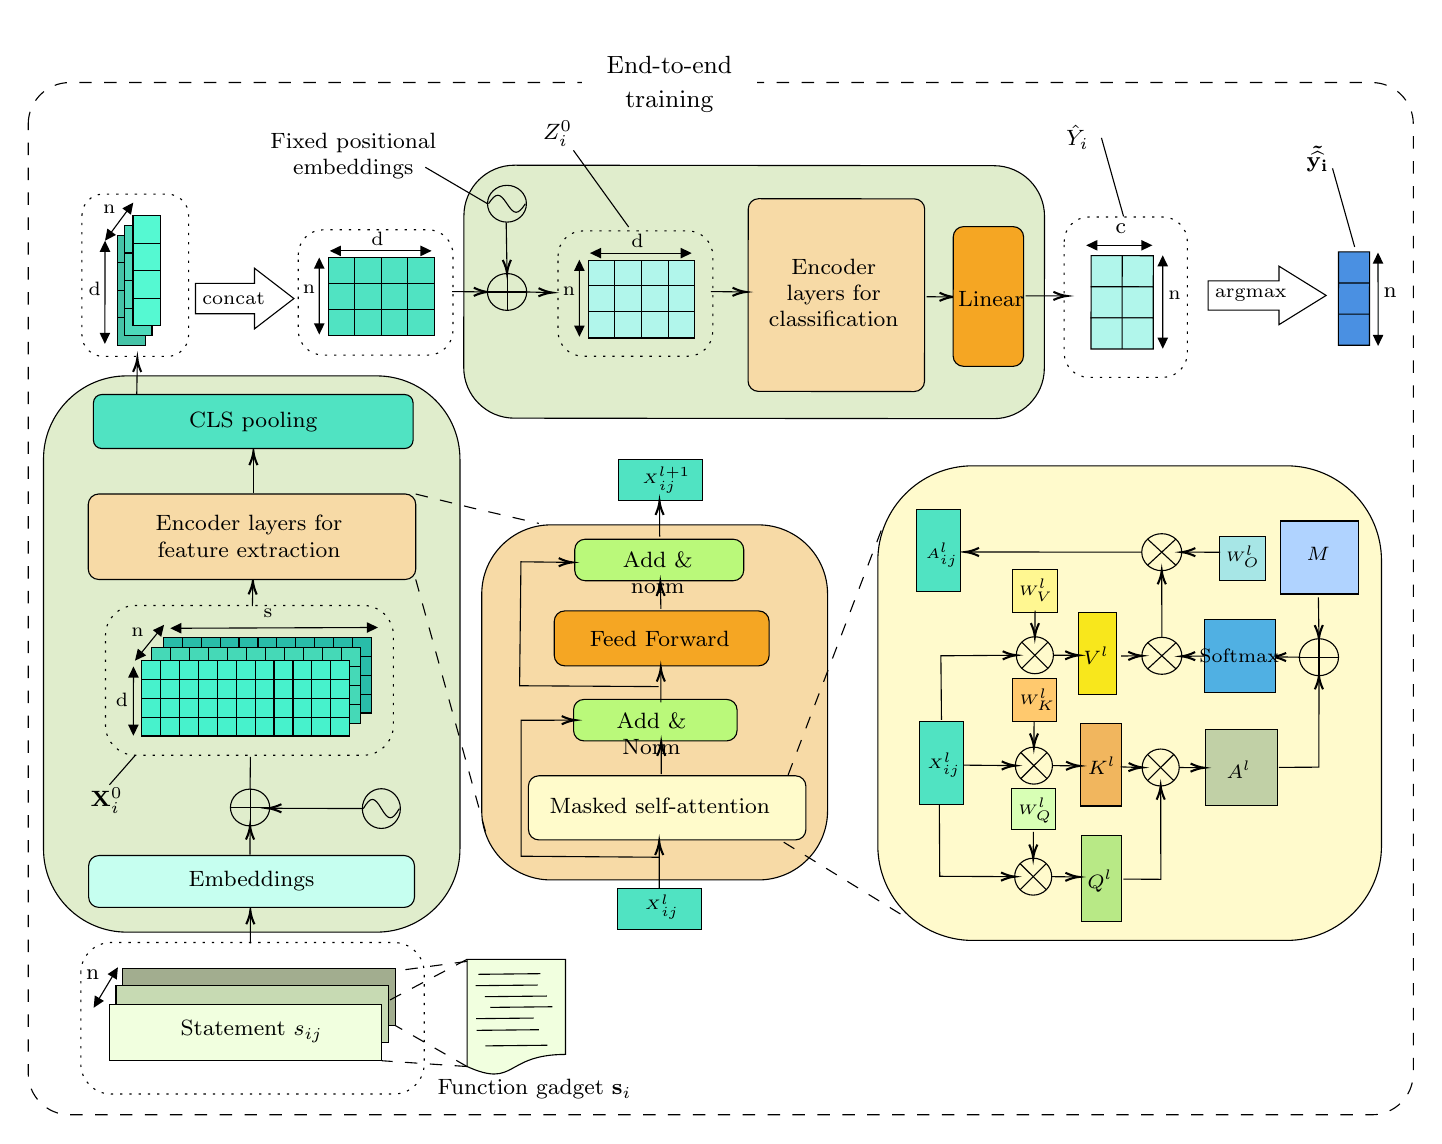
\begin{tikzpicture}[x=0.75pt,y=0.75pt,yscale=-1,xscale=1]
%uncomment if require: \path (0,582); %set diagram left start at 0, and has height of 582

%Rounded Rect [id:dp40408364631982896] 
\draw  [fill={rgb, 255:red, 247; green, 218; blue, 166 }  ,fill opacity=1 ] (245.5,285.63) .. controls (245.5,267.22) and (260.42,252.3) .. (278.83,252.3) -- (378.8,252.3) .. controls (397.2,252.3) and (412.12,267.22) .. (412.12,285.63) -- (412.12,390.04) .. controls (412.12,408.45) and (397.2,423.37) .. (378.8,423.37) -- (278.83,423.37) .. controls (260.42,423.37) and (245.5,408.45) .. (245.5,390.04) -- cycle ;
%Rounded Rect [id:dp44940872081608707] 
\draw  [fill={rgb, 255:red, 255; green, 250; blue, 204 }  ,fill opacity=1 ] (436.33,269.59) .. controls (436.33,244.33) and (456.81,223.85) .. (482.07,223.85) -- (633.27,223.85) .. controls (658.52,223.85) and (679,244.33) .. (679,269.59) -- (679,406.79) .. controls (679,432.05) and (658.52,452.52) .. (633.27,452.52) -- (482.07,452.52) .. controls (456.81,452.52) and (436.33,432.05) .. (436.33,406.79) -- cycle ;
%Shape: Rectangle [id:dp562618901702713] 
\draw  [fill={rgb, 255:red, 176; green, 211; blue, 255 }  ,fill opacity=1 ] (630.27,250.42) -- (667.78,250.42) -- (667.78,285.62) -- (630.27,285.62) -- cycle ;

%Shape: Rectangle [id:dp38860883770971566] 
\draw  [fill={rgb, 255:red, 193; green, 208; blue, 166 }  ,fill opacity=1 ] (594.15,350.79) -- (628.75,350.79) -- (628.75,387.3) -- (594.15,387.3) -- cycle ;
%Shape: Rectangle [id:dp21600716570430678] 
\draw  [fill={rgb, 255:red, 241; green, 182; blue, 94 }  ,fill opacity=1 ] (534.11,348.05) -- (553.84,348.05) -- (553.84,387.73) -- (534.11,387.73) -- cycle ;
%Shape: Rectangle [id:dp8193196680097512] 
\draw  [fill={rgb, 255:red, 184; green, 233; blue, 134 }  ,fill opacity=1 ] (534.53,401.95) -- (553.84,401.95) -- (553.84,443.39) -- (534.53,443.39) -- cycle ;
%Shape: Rectangle [id:dp1477324685865582] 
\draw  [fill={rgb, 255:red, 248; green, 231; blue, 28 }  ,fill opacity=1 ] (532.95,294.54) -- (551.29,294.54) -- (551.29,334.22) -- (532.95,334.22) -- cycle ;

%Straight Lines [id:da40715388627553684] 
\draw    (477.71,368.06) -- (500.59,368.27) ;
\draw [shift={(502.59,368.29)}, rotate = 180.54] [color={rgb, 255:red, 0; green, 0; blue, 0 }  ][line width=0.75]    (6.56,-1.97) .. controls (4.17,-0.84) and (1.99,-0.18) .. (0,0) .. controls (1.99,0.18) and (4.17,0.84) .. (6.56,1.97)   ;
%Straight Lines [id:da3948086408555571] 
\draw    (467,346.24) -- (466.71,315.38) -- (501.06,315.12) ;
\draw [shift={(503.06,315.11)}, rotate = 179.58] [color={rgb, 255:red, 0; green, 0; blue, 0 }  ][line width=0.75]    (6.56,-1.97) .. controls (4.17,-0.84) and (1.99,-0.18) .. (0,0) .. controls (1.99,0.18) and (4.17,0.84) .. (6.56,1.97)   ;
%Straight Lines [id:da6628678611462153] 
\draw    (465.97,386.65) -- (466.15,421.61) -- (500.26,421.78) ;
\draw [shift={(502.26,421.79)}, rotate = 180.29] [color={rgb, 255:red, 0; green, 0; blue, 0 }  ][line width=0.75]    (6.56,-1.97) .. controls (4.17,-0.84) and (1.99,-0.18) .. (0,0) .. controls (1.99,0.18) and (4.17,0.84) .. (6.56,1.97)   ;
%Flowchart: Summing Junction [id:dp08207128645404782] 
\draw   (563.68,369.2) .. controls (563.68,364.29) and (567.68,360.3) .. (572.61,360.3) .. controls (577.54,360.3) and (581.54,364.29) .. (581.54,369.2) .. controls (581.54,374.12) and (577.54,378.11) .. (572.61,378.11) .. controls (567.68,378.11) and (563.68,374.12) .. (563.68,369.2) -- cycle ; \draw   (566.3,362.91) -- (578.93,375.5) ; \draw   (578.93,362.91) -- (566.3,375.5) ;
%Flowchart: Or [id:dp24850160031696777] 
\draw   (639.44,316.06) .. controls (639.44,311.14) and (643.66,307.16) .. (648.86,307.16) .. controls (654.07,307.16) and (658.29,311.14) .. (658.29,316.06) .. controls (658.29,320.98) and (654.07,324.96) .. (648.86,324.96) .. controls (643.66,324.96) and (639.44,320.98) .. (639.44,316.06) -- cycle ; \draw   (639.44,316.06) -- (658.29,316.06) ; \draw   (648.86,307.16) -- (648.86,324.96) ;
%Straight Lines [id:da8436563002880748] 
\draw    (553.34,368.9) -- (561.68,369.15) ;
\draw [shift={(563.68,369.2)}, rotate = 181.68] [color={rgb, 255:red, 0; green, 0; blue, 0 }  ][line width=0.75]    (6.56,-1.97) .. controls (4.17,-0.84) and (1.99,-0.18) .. (0,0) .. controls (1.99,0.18) and (4.17,0.84) .. (6.56,1.97)   ;
%Straight Lines [id:da5866395823147741] 
\draw    (554.69,422.96) -- (572.69,423.07) -- (572.61,380.11) ;
\draw [shift={(572.61,378.11)}, rotate = 89.9] [color={rgb, 255:red, 0; green, 0; blue, 0 }  ][line width=0.75]    (6.56,-1.97) .. controls (4.17,-0.84) and (1.99,-0.18) .. (0,0) .. controls (1.99,0.18) and (4.17,0.84) .. (6.56,1.97)   ;
%Straight Lines [id:da5467028367044005] 
\draw    (581.54,369.2) -- (591.58,369.31) ;
\draw [shift={(593.58,369.33)}, rotate = 180.62] [color={rgb, 255:red, 0; green, 0; blue, 0 }  ][line width=0.75]    (6.56,-1.97) .. controls (4.17,-0.84) and (1.99,-0.18) .. (0,0) .. controls (1.99,0.18) and (4.17,0.84) .. (6.56,1.97)   ;
%Straight Lines [id:da45559947633695286] 
\draw    (628.47,315.91) -- (639.44,316.06) ;
\draw [shift={(626.47,315.89)}, rotate = 0.76] [color={rgb, 255:red, 0; green, 0; blue, 0 }  ][line width=0.75]    (6.56,-1.97) .. controls (4.17,-0.84) and (1.99,-0.18) .. (0,0) .. controls (1.99,0.18) and (4.17,0.84) .. (6.56,1.97)   ;
%Flowchart: Summing Junction [id:dp6374896002896995] 
\draw   (563.56,315.38) .. controls (563.56,310.47) and (567.86,306.48) .. (573.18,306.48) .. controls (578.49,306.48) and (582.8,310.47) .. (582.8,315.38) .. controls (582.8,320.3) and (578.49,324.29) .. (573.18,324.29) .. controls (567.86,324.29) and (563.56,320.3) .. (563.56,315.38) -- cycle ; \draw   (566.37,309.09) -- (579.98,321.68) ; \draw   (579.98,309.09) -- (566.37,321.68) ;
%Straight Lines [id:da5838051153778354] 
\draw    (553.55,315.49) -- (561.56,315.4) ;
\draw [shift={(563.56,315.38)}, rotate = 179.42] [color={rgb, 255:red, 0; green, 0; blue, 0 }  ][line width=0.75]    (6.56,-1.97) .. controls (4.17,-0.84) and (1.99,-0.18) .. (0,0) .. controls (1.99,0.18) and (4.17,0.84) .. (6.56,1.97)   ;
%Straight Lines [id:da3997608796060319] 
\draw    (629.58,369.15) -- (648.85,369.03) -- (648.86,342.19) -- (648.86,326.96) ;
\draw [shift={(648.86,324.96)}, rotate = 90.02] [color={rgb, 255:red, 0; green, 0; blue, 0 }  ][line width=0.75]    (6.56,-1.97) .. controls (4.17,-0.84) and (1.99,-0.18) .. (0,0) .. controls (1.99,0.18) and (4.17,0.84) .. (6.56,1.97)   ;
%Straight Lines [id:da38354296286226863] 
\draw    (593.53,315.49) -- (584.65,315.61) ;
\draw [shift={(582.65,315.64)}, rotate = 359.21] [color={rgb, 255:red, 0; green, 0; blue, 0 }  ][line width=0.75]    (6.56,-1.97) .. controls (4.17,-0.84) and (1.99,-0.18) .. (0,0) .. controls (1.99,0.18) and (4.17,0.84) .. (6.56,1.97)   ;
%Flowchart: Summing Junction [id:dp4337356590843586] 
\draw   (503.06,315.11) .. controls (503.06,310.19) and (507.06,306.21) .. (511.99,306.21) .. controls (516.93,306.21) and (520.93,310.19) .. (520.93,315.11) .. controls (520.93,320.03) and (516.93,324.01) .. (511.99,324.01) .. controls (507.06,324.01) and (503.06,320.03) .. (503.06,315.11) -- cycle ; \draw   (505.68,308.81) -- (518.31,321.4) ; \draw   (518.31,308.81) -- (505.68,321.4) ;
%Flowchart: Summing Junction [id:dp06181836266069829] 
\draw   (502.59,368.29) .. controls (502.59,363.38) and (506.59,359.39) .. (511.52,359.39) .. controls (516.45,359.39) and (520.45,363.38) .. (520.45,368.29) .. controls (520.45,373.21) and (516.45,377.2) .. (511.52,377.2) .. controls (506.59,377.2) and (502.59,373.21) .. (502.59,368.29) -- cycle ; \draw   (505.21,362) -- (517.84,374.59) ; \draw   (517.84,362) -- (505.21,374.59) ;
%Straight Lines [id:da7798924033944554] 
\draw    (511.62,346.74) -- (511.54,357.39) ;
\draw [shift={(511.52,359.39)}, rotate = 270.43] [color={rgb, 255:red, 0; green, 0; blue, 0 }  ][line width=0.75]    (6.56,-1.97) .. controls (4.17,-0.84) and (1.99,-0.18) .. (0,0) .. controls (1.99,0.18) and (4.17,0.84) .. (6.56,1.97)   ;
%Straight Lines [id:da27285248678093654] 
\draw    (520.45,368.29) -- (531.59,368.41) ;
\draw [shift={(533.59,368.43)}, rotate = 180.6] [color={rgb, 255:red, 0; green, 0; blue, 0 }  ][line width=0.75]    (6.56,-1.97) .. controls (4.17,-0.84) and (1.99,-0.18) .. (0,0) .. controls (1.99,0.18) and (4.17,0.84) .. (6.56,1.97)   ;
%Shape: Rectangle [id:dp056052511629974155] 
\draw  [fill={rgb, 255:red, 255; green, 247; blue, 145 }  ,fill opacity=1 ] (501.06,273.77) -- (522.9,273.77) -- (522.9,294.34) -- (501.06,294.34) -- cycle ;
%Flowchart: Summing Junction [id:dp9747068518892847] 
\draw   (502.26,421.79) .. controls (502.26,416.88) and (506.26,412.89) .. (511.19,412.89) .. controls (516.12,412.89) and (520.12,416.88) .. (520.12,421.79) .. controls (520.12,426.71) and (516.12,430.69) .. (511.19,430.69) .. controls (506.26,430.69) and (502.26,426.71) .. (502.26,421.79) -- cycle ; \draw   (504.88,415.5) -- (517.51,428.09) ; \draw   (517.51,415.5) -- (504.88,428.09) ;
%Straight Lines [id:da77518906522465] 
\draw    (512.09,293.56) -- (512.01,304.21) ;
\draw [shift={(511.99,306.21)}, rotate = 270.43] [color={rgb, 255:red, 0; green, 0; blue, 0 }  ][line width=0.75]    (6.56,-1.97) .. controls (4.17,-0.84) and (1.99,-0.18) .. (0,0) .. controls (1.99,0.18) and (4.17,0.84) .. (6.56,1.97)   ;
%Straight Lines [id:da8462353829933633] 
\draw    (511.29,400.24) -- (511.21,410.89) ;
\draw [shift={(511.19,412.89)}, rotate = 270.43] [color={rgb, 255:red, 0; green, 0; blue, 0 }  ][line width=0.75]    (6.56,-1.97) .. controls (4.17,-0.84) and (1.99,-0.18) .. (0,0) .. controls (1.99,0.18) and (4.17,0.84) .. (6.56,1.97)   ;
%Straight Lines [id:da39065485951471146] 
\draw    (531.16,315.14) -- (520.93,315.11) ;
\draw [shift={(533.16,315.15)}, rotate = 180.2] [color={rgb, 255:red, 0; green, 0; blue, 0 }  ][line width=0.75]    (6.56,-1.97) .. controls (4.17,-0.84) and (1.99,-0.18) .. (0,0) .. controls (1.99,0.18) and (4.17,0.84) .. (6.56,1.97)   ;
%Shape: Rectangle [id:dp7396954307330748] 
\draw  [fill={rgb, 255:red, 255; green, 201; blue, 110 }  ,fill opacity=1 ] (501.31,326.43) -- (522.56,326.43) -- (522.56,347) -- (501.31,347) -- cycle ;
%Shape: Rectangle [id:dp2957808463352003] 
\draw  [fill={rgb, 255:red, 216; green, 255; blue, 181 }  ,fill opacity=1 ] (500.7,379.35) -- (521.73,379.35) -- (521.73,399.21) -- (500.7,399.21) -- cycle ;
%Straight Lines [id:da6424235489998926] 
\draw    (520.12,421.79) -- (531.26,421.91) ;
\draw [shift={(533.26,421.93)}, rotate = 180.6] [color={rgb, 255:red, 0; green, 0; blue, 0 }  ][line width=0.75]    (6.56,-1.97) .. controls (4.17,-0.84) and (1.99,-0.18) .. (0,0) .. controls (1.99,0.18) and (4.17,0.84) .. (6.56,1.97)   ;
%Shape: Rectangle [id:dp10325192922634319] 
\draw  [fill={rgb, 255:red, 80; green, 227; blue, 194 }  ,fill opacity=1 ] (456.34,347.21) -- (477.47,347.21) -- (477.47,386.89) -- (456.34,386.89) -- cycle ;
%Flowchart: Summing Junction [id:dp927545824744036] 
\draw   (563.5,265.45) .. controls (563.5,260.54) and (567.8,256.55) .. (573.12,256.55) .. controls (578.43,256.55) and (582.74,260.54) .. (582.74,265.45) .. controls (582.74,270.37) and (578.43,274.36) .. (573.12,274.36) .. controls (567.8,274.36) and (563.5,270.37) .. (563.5,265.45) -- cycle ; \draw   (566.31,259.16) -- (579.92,271.75) ; \draw   (579.92,259.16) -- (566.31,271.75) ;
%Shape: Rectangle [id:dp6713108345262884] 
\draw  [fill={rgb, 255:red, 167; green, 230; blue, 230 }  ,fill opacity=1 ] (600.83,257.71) -- (623.02,257.71) -- (623.02,279.09) -- (600.83,279.09) -- cycle ;
%Straight Lines [id:da5399778406458415] 
\draw    (573.18,306.48) -- (573.12,276.36) ;
\draw [shift={(573.12,274.36)}, rotate = 89.89] [color={rgb, 255:red, 0; green, 0; blue, 0 }  ][line width=0.75]    (6.56,-1.97) .. controls (4.17,-0.84) and (1.99,-0.18) .. (0,0) .. controls (1.99,0.18) and (4.17,0.84) .. (6.56,1.97)   ;
%Straight Lines [id:da7965017454833045] 
\draw    (563.5,265.45) -- (480.51,265.36) ;
\draw [shift={(478.51,265.36)}, rotate = 0.07] [color={rgb, 255:red, 0; green, 0; blue, 0 }  ][line width=0.75]    (6.56,-1.97) .. controls (4.17,-0.84) and (1.99,-0.18) .. (0,0) .. controls (1.99,0.18) and (4.17,0.84) .. (6.56,1.97)   ;
%Straight Lines [id:da7999314726696041] 
\draw    (601.19,265.47) -- (584.74,265.46) ;
\draw [shift={(582.74,265.45)}, rotate = 0.06] [color={rgb, 255:red, 0; green, 0; blue, 0 }  ][line width=0.75]    (6.56,-1.97) .. controls (4.17,-0.84) and (1.99,-0.18) .. (0,0) .. controls (1.99,0.18) and (4.17,0.84) .. (6.56,1.97)   ;
%Shape: Rectangle [id:dp9722051619567833] 
\draw  [fill={rgb, 255:red, 80; green, 176; blue, 227 }  ,fill opacity=1 ] (593.53,297.91) -- (628.06,297.91) -- (628.06,333.14) -- (593.53,333.14) -- cycle ;
%Straight Lines [id:da32261209503586485] 
\draw    (648.84,305.16) -- (648.6,287.27) ;
\draw [shift={(648.86,307.16)}, rotate = 269.25] [color={rgb, 255:red, 0; green, 0; blue, 0 }  ][line width=0.75]    (6.56,-1.97) .. controls (4.17,-0.84) and (1.99,-0.18) .. (0,0) .. controls (1.99,0.18) and (4.17,0.84) .. (6.56,1.97)   ;
%Shape: Rectangle [id:dp14061707702777704] 
\draw  [fill={rgb, 255:red, 80; green, 227; blue, 194 }  ,fill opacity=1 ] (454.9,244.71) -- (476.04,244.71) -- (476.04,284.39) -- (454.9,284.39) -- cycle ;
%Shape: Rectangle [id:dp3851600003577855] 
\draw  [fill={rgb, 255:red, 80; green, 227; blue, 194 }  ,fill opacity=1 ] (310.86,427.34) -- (351.53,427.34) -- (351.53,447.13) -- (310.86,447.13) -- cycle ;
%Rounded Rect [id:dp27042387264364565] 
\draw  [fill={rgb, 255:red, 224; green, 237; blue, 204 }  ,fill opacity=1 ] (34.36,220.65) .. controls (34.36,198.49) and (52.32,180.52) .. (74.49,180.52) -- (194.87,180.52) .. controls (217.03,180.52) and (235,198.49) .. (235,220.65) -- (235,408.39) .. controls (235,430.55) and (217.03,448.52) .. (194.87,448.52) -- (74.49,448.52) .. controls (52.32,448.52) and (34.36,430.55) .. (34.36,408.39) -- cycle ;
%Rounded Rect [id:dp06487154210447232] 
\draw  [fill={rgb, 255:red, 224; green, 237; blue, 204 }  ,fill opacity=1 ] (236.91,103.36) .. controls (236.93,89.9) and (247.85,78.99) .. (261.31,79.01) -- (492.29,79.25) .. controls (505.75,79.26) and (516.65,90.19) .. (516.64,103.65) -- (516.56,176.78) .. controls (516.55,190.25) and (505.62,201.15) .. (492.16,201.13) -- (261.19,200.89) .. controls (247.72,200.88) and (236.82,189.95) .. (236.83,176.49) -- cycle ;
%Shape: Grid [id:dp7302897233495353] 
\draw  [draw opacity=0][fill={rgb, 255:red, 80; green, 227; blue, 194 }  ,fill opacity=1 ] (171.51,123.69) -- (222.74,123.69) -- (222.74,136.5) -- (171.51,136.5) -- cycle ; \draw   (184.32,123.69) -- (184.32,136.5)(197.13,123.69) -- (197.13,136.5)(209.93,123.69) -- (209.93,136.5) ; \draw    ; \draw   (171.51,123.69) -- (222.74,123.69) -- (222.74,136.5) -- (171.51,136.5) -- cycle ;
%Shape: Grid [id:dp8395667427331548] 
\draw  [draw opacity=0][fill={rgb, 255:red, 80; green, 227; blue, 194 }  ,fill opacity=1 ] (171.51,136.04) -- (222.74,136.04) -- (222.74,148.85) -- (171.51,148.85) -- cycle ; \draw   (184.32,136.04) -- (184.32,148.85)(197.13,136.04) -- (197.13,148.85)(209.93,136.04) -- (209.93,148.85) ; \draw    ; \draw   (171.51,136.04) -- (222.74,136.04) -- (222.74,148.85) -- (171.51,148.85) -- cycle ;
%Shape: Grid [id:dp7617245535835451] 
\draw  [draw opacity=0][fill={rgb, 255:red, 80; green, 227; blue, 194 }  ,fill opacity=1 ] (171.51,148.39) -- (222.74,148.39) -- (222.74,161.2) -- (171.51,161.2) -- cycle ; \draw   (184.32,148.39) -- (184.32,161.2)(197.13,148.39) -- (197.13,161.2)(209.93,148.39) -- (209.93,161.2) ; \draw    ; \draw   (171.51,148.39) -- (222.74,148.39) -- (222.74,161.2) -- (171.51,161.2) -- cycle ;
%Rounded Rect [id:dp5740799340916567] 
\draw  [dash pattern={on 0.84pt off 2.51pt}] (157.1,122.21) .. controls (157.1,115.54) and (162.5,110.13) .. (169.17,110.13) -- (219.59,110.13) .. controls (226.26,110.13) and (231.67,115.54) .. (231.67,122.21) -- (231.67,158.44) .. controls (231.67,165.11) and (226.26,170.52) .. (219.59,170.52) -- (169.17,170.52) .. controls (162.5,170.52) and (157.1,165.11) .. (157.1,158.44) -- cycle ;
%Straight Lines [id:da33020866172978813] 
\draw    (167.23,157.59) -- (167.2,126.49) ;
\draw [shift={(167.2,123.49)}, rotate = 89.95] [fill={rgb, 255:red, 0; green, 0; blue, 0 }  ][line width=0.08]  [draw opacity=0] (5.36,-2.57) -- (0,0) -- (5.36,2.57) -- cycle    ;
\draw [shift={(167.23,160.59)}, rotate = 269.95] [fill={rgb, 255:red, 0; green, 0; blue, 0 }  ][line width=0.08]  [draw opacity=0] (5.36,-2.57) -- (0,0) -- (5.36,2.57) -- cycle    ;
%Straight Lines [id:da6834662447393993] 
\draw    (218.34,120.3) -- (175.31,120.3) ;
\draw [shift={(172.31,120.3)}, rotate = 360] [fill={rgb, 255:red, 0; green, 0; blue, 0 }  ][line width=0.08]  [draw opacity=0] (5.36,-2.57) -- (0,0) -- (5.36,2.57) -- cycle    ;
\draw [shift={(221.34,120.3)}, rotate = 180] [fill={rgb, 255:red, 0; green, 0; blue, 0 }  ][line width=0.08]  [draw opacity=0] (5.36,-2.57) -- (0,0) -- (5.36,2.57) -- cycle    ;
%Shape: Sine Wave Form [id:dp913545478885857] 
\draw   (248.78,97.57) .. controls (252.4,92.14) and (254.1,92.11) .. (257.66,97.58) .. controls (261.21,103.05) and (262.88,103.08) .. (266.54,97.59) ;
%Shape: Ellipse [id:dp03640208207764273] 
\draw   (248.28,97.57) .. controls (248.29,92.67) and (252.49,88.71) .. (257.67,88.71) .. controls (262.84,88.72) and (267.03,92.69) .. (267.03,97.59) .. controls (267.02,102.48) and (262.82,106.45) .. (257.65,106.44) .. controls (252.47,106.44) and (248.28,102.46) .. (248.28,97.57) -- cycle ;

%Shape: Sine Wave Form [id:dp3018436347412632] 
\draw   (188.45,388.98) .. controls (191.98,383.11) and (193.65,383.08) .. (197.13,388.98) .. controls (200.62,394.88) and (202.25,394.92) .. (205.82,388.98) ;
%Shape: Ellipse [id:dp33480574729419144] 
\draw   (187.97,388.98) .. controls (187.97,383.69) and (192.07,379.41) .. (197.13,379.41) .. controls (202.19,379.41) and (206.3,383.69) .. (206.3,388.98) .. controls (206.3,394.27) and (202.19,398.56) .. (197.13,398.56) .. controls (192.07,398.56) and (187.97,394.27) .. (187.97,388.98) -- cycle ;

%Straight Lines [id:da17601389428006953] 
\draw    (188.45,388.98) -- (144.42,388.84) ;
\draw [shift={(142.42,388.83)}, rotate = 0.19] [color={rgb, 255:red, 0; green, 0; blue, 0 }  ][line width=0.75]    (6.56,-1.97) .. controls (4.17,-0.84) and (1.99,-0.18) .. (0,0) .. controls (1.99,0.18) and (4.17,0.84) .. (6.56,1.97)   ;
%Straight Lines [id:da9327052133654938] 
\draw    (135,291.44) -- (135.2,281.24) ;
\draw [shift={(135.24,279.24)}, rotate = 91.15] [color={rgb, 255:red, 0; green, 0; blue, 0 }  ][line width=0.75]    (6.56,-1.97) .. controls (4.17,-0.84) and (1.99,-0.18) .. (0,0) .. controls (1.99,0.18) and (4.17,0.84) .. (6.56,1.97)   ;
%Straight Lines [id:da28107434708891144] 
\draw    (133.86,411.13) -- (133.88,399.34) ;
\draw [shift={(133.88,397.34)}, rotate = 90.09] [color={rgb, 255:red, 0; green, 0; blue, 0 }  ][line width=0.75]    (6.56,-1.97) .. controls (4.17,-0.84) and (1.99,-0.18) .. (0,0) .. controls (1.99,0.18) and (4.17,0.84) .. (6.56,1.97)   ;
%Straight Lines [id:da011852462880014514] 
\draw    (133.88,379.61) -- (134.05,364.11) ;
%Straight Lines [id:da7442516062798874] 
\draw    (79.28,190.02) -- (79.54,174.04) ;
\draw [shift={(79.57,172.04)}, rotate = 90.91] [color={rgb, 255:red, 0; green, 0; blue, 0 }  ][line width=0.75]    (6.56,-1.97) .. controls (4.17,-0.84) and (1.99,-0.18) .. (0,0) .. controls (1.99,0.18) and (4.17,0.84) .. (6.56,1.97)   ;
%Shape: Grid [id:dp09962250431195896] 
\draw  [draw opacity=0][fill={rgb, 255:red, 177; green, 246; blue, 235 }  ,fill opacity=1 ] (539.09,122.59) -- (569.06,122.62) -- (569.05,137.61) -- (539.07,137.57) -- cycle ; \draw   (554.08,122.6) -- (554.06,137.59) ; \draw    ; \draw   (539.09,122.59) -- (569.06,122.62) -- (569.05,137.61) -- (539.07,137.57) -- cycle ;
%Shape: Grid [id:dp6390212974381149] 
\draw  [draw opacity=0][fill={rgb, 255:red, 177; green, 246; blue, 235 }  ,fill opacity=1 ] (539.07,137.57) -- (569.05,137.61) -- (569.03,152.59) -- (539.06,152.56) -- cycle ; \draw   (554.06,137.59) -- (554.05,152.58) ; \draw    ; \draw   (539.07,137.57) -- (569.05,137.61) -- (569.03,152.59) -- (539.06,152.56) -- cycle ;
%Shape: Grid [id:dp8807483145189927] 
\draw  [draw opacity=0][fill={rgb, 255:red, 177; green, 246; blue, 235 }  ,fill opacity=1 ] (539.06,152.56) -- (569.03,152.59) -- (569.02,167.58) -- (539.04,167.55) -- cycle ; \draw   (554.05,152.58) -- (554.03,167.56) ; \draw    ; \draw   (539.06,152.56) -- (569.03,152.59) -- (569.02,167.58) -- (539.04,167.55) -- cycle ;
%Straight Lines [id:da9413914317582963] 
\draw [fill={rgb, 255:red, 80; green, 227; blue, 194 }  ,fill opacity=1 ]   (565.62,117.61) -- (539.74,117.61) ;
\draw [shift={(536.74,117.61)}, rotate = 360] [fill={rgb, 255:red, 0; green, 0; blue, 0 }  ][line width=0.08]  [draw opacity=0] (5.36,-2.57) -- (0,0) -- (5.36,2.57) -- cycle    ;
\draw [shift={(568.62,117.61)}, rotate = 180] [fill={rgb, 255:red, 0; green, 0; blue, 0 }  ][line width=0.08]  [draw opacity=0] (5.36,-2.57) -- (0,0) -- (5.36,2.57) -- cycle    ;
%Straight Lines [id:da9554784172752084] 
\draw [fill={rgb, 255:red, 80; green, 227; blue, 194 }  ,fill opacity=1 ]   (573.62,164.44) -- (573.59,125.42) ;
\draw [shift={(573.59,122.42)}, rotate = 89.95] [fill={rgb, 255:red, 0; green, 0; blue, 0 }  ][line width=0.08]  [draw opacity=0] (5.36,-2.57) -- (0,0) -- (5.36,2.57) -- cycle    ;
\draw [shift={(573.62,167.44)}, rotate = 269.95] [fill={rgb, 255:red, 0; green, 0; blue, 0 }  ][line width=0.08]  [draw opacity=0] (5.36,-2.57) -- (0,0) -- (5.36,2.57) -- cycle    ;
%Rounded Rect [id:dp7957747950328782] 
\draw  [dash pattern={on 0.84pt off 2.51pt}] (526.12,115.85) .. controls (526.12,109.29) and (531.43,103.98) .. (537.99,103.98) -- (573.61,103.98) .. controls (580.17,103.98) and (585.48,109.29) .. (585.48,115.85) -- (585.48,169.36) .. controls (585.48,175.92) and (580.17,181.24) .. (573.61,181.24) -- (537.99,181.24) .. controls (531.43,181.24) and (526.12,175.92) .. (526.12,169.36) -- cycle ;
%Shape: Rectangle [id:dp3541253672827793] 
\draw  [fill={rgb, 255:red, 247; green, 218; blue, 166 }  ,fill opacity=1 ] (373.89,100.14) .. controls (373.89,97.38) and (376.14,95.15) .. (378.9,95.15) -- (453.92,95.23) .. controls (456.68,95.23) and (458.92,97.47) .. (458.91,100.23) -- (458.83,183.08) .. controls (458.82,185.84) and (456.58,188.07) .. (453.82,188.07) -- (378.8,187.99) .. controls (376.04,187.99) and (373.8,185.75) .. (373.81,182.99) -- cycle ;
%Straight Lines [id:da7363088519141203] 
\draw    (459.8,142.39) -- (470.64,142.46) ;
\draw [shift={(472.64,142.47)}, rotate = 180.37] [color={rgb, 255:red, 0; green, 0; blue, 0 }  ][line width=0.75]    (6.56,-1.97) .. controls (4.17,-0.84) and (1.99,-0.18) .. (0,0) .. controls (1.99,0.18) and (4.17,0.84) .. (6.56,1.97)   ;
%Straight Lines [id:da9144669808851449] 
\draw    (267.16,140.09) -- (277.4,140.34) ;
\draw [shift={(279.4,140.39)}, rotate = 181.41] [color={rgb, 255:red, 0; green, 0; blue, 0 }  ][line width=0.75]    (6.56,-1.97) .. controls (4.17,-0.84) and (1.99,-0.18) .. (0,0) .. controls (1.99,0.18) and (4.17,0.84) .. (6.56,1.97)   ;
%Straight Lines [id:da3061968060397451] 
\draw    (257.28,106.66) -- (257.66,129.22) ;
\draw [shift={(257.7,131.22)}, rotate = 269.02] [color={rgb, 255:red, 0; green, 0; blue, 0 }  ][line width=0.75]    (6.56,-1.97) .. controls (4.17,-0.84) and (1.99,-0.18) .. (0,0) .. controls (1.99,0.18) and (4.17,0.84) .. (6.56,1.97)   ;
%Shape: Rectangle [id:dp5612435545000494] 
\draw  [fill={rgb, 255:red, 162; green, 173; blue, 143 }  ,fill opacity=1 ] (72.5,466.25) -- (203.81,466.25) -- (203.81,493.49) -- (72.5,493.49) -- cycle ;
%Shape: Rectangle [id:dp3874409957215059] 
\draw  [fill={rgb, 255:red, 199; green, 218; blue, 179 }  ,fill opacity=1 ] (69.29,474.26) -- (200.6,474.26) -- (200.6,501.5) -- (69.29,501.5) -- cycle ;
%Shape: Rectangle [id:dp7444242621133832] 
\draw  [fill={rgb, 255:red, 241; green, 255; blue, 223 }  ,fill opacity=1 ] (66.07,483.24) -- (197.39,483.24) -- (197.39,510.48) -- (66.07,510.48) -- cycle ;
%Flowchart: Document [id:dp6610270108906255] 
\draw  [fill={rgb, 255:red, 241; green, 255; blue, 223 }  ,fill opacity=1 ] (238.45,461.61) -- (285.84,461.61) -- (285.84,507.44) .. controls (256.22,507.44) and (262.14,523.96) .. (238.45,513.27) -- cycle ;
%Straight Lines [id:da40772950605873826] 
\draw [fill={rgb, 255:red, 241; green, 255; blue, 223 }  ,fill opacity=1 ]   (249.6,484.78) -- (279.51,484.47) ;
%Straight Lines [id:da619620129362211] 
\draw [fill={rgb, 255:red, 241; green, 255; blue, 223 }  ,fill opacity=1 ]   (242.79,490.2) -- (270.55,489.91) ;

%Straight Lines [id:da11569866109659155] 
\draw [fill={rgb, 255:red, 241; green, 255; blue, 223 }  ,fill opacity=1 ]   (243.84,468.84) -- (273.74,468.53) ;
%Straight Lines [id:da49540992658715677] 
\draw [fill={rgb, 255:red, 241; green, 255; blue, 223 }  ,fill opacity=1 ]   (242.57,474.32) -- (272.48,474.01) ;
%Straight Lines [id:da40560150360570546] 
\draw [fill={rgb, 255:red, 241; green, 255; blue, 223 }  ,fill opacity=1 ]   (247,479.62) -- (276.91,479.31) ;
%Straight Lines [id:da6508111653914503] 
\draw [fill={rgb, 255:red, 241; green, 255; blue, 223 }  ,fill opacity=1 ]   (243.06,495.84) -- (272.97,495.53) ;
%Straight Lines [id:da25442117472960724] 
\draw [fill={rgb, 255:red, 241; green, 255; blue, 223 }  ,fill opacity=1 ]   (247.25,503.32) -- (277.16,503.01) ;

%Straight Lines [id:da7811882134425123] 
\draw  [dash pattern={on 4.5pt off 4.5pt}]  (238.45,461.61) -- (197.39,483.24) ;
%Straight Lines [id:da5040308898211101] 
\draw  [dash pattern={on 4.5pt off 4.5pt}]  (238.45,513.27) -- (197.39,510.48) ;
%Straight Lines [id:da19325202309674538] 
\draw  [dash pattern={on 4.5pt off 4.5pt}]  (238.45,513.27) -- (203.81,493.49) ;
%Rounded Rect [id:dp7839876975702906] 
\draw  [dash pattern={on 0.84pt off 2.51pt}] (52.33,468.11) .. controls (52.33,460.04) and (58.87,453.51) .. (66.94,453.51) -- (203.18,453.51) .. controls (211.25,453.51) and (217.79,460.04) .. (217.79,468.11) -- (217.79,511.92) .. controls (217.79,519.98) and (211.25,526.52) .. (203.18,526.52) -- (66.94,526.52) .. controls (58.87,526.52) and (52.33,519.98) .. (52.33,511.92) -- cycle ;
%Straight Lines [id:da404920413339354] 
\draw    (134,453.94) -- (134.02,440.14) ;
\draw [shift={(134.02,438.14)}, rotate = 90.06] [color={rgb, 255:red, 0; green, 0; blue, 0 }  ][line width=0.75]    (6.56,-1.97) .. controls (4.17,-0.84) and (1.99,-0.18) .. (0,0) .. controls (1.99,0.18) and (4.17,0.84) .. (6.56,1.97)   ;
%Shape: Rectangle [id:dp48949706720977715] 
\draw  [fill={rgb, 255:red, 247; green, 218; blue, 166 }  ,fill opacity=1 ] (55.93,242.44) .. controls (55.93,239.68) and (58.17,237.44) .. (60.93,237.44) -- (208.7,237.44) .. controls (211.46,237.44) and (213.7,239.68) .. (213.7,242.44) -- (213.7,273.6) .. controls (213.7,276.37) and (211.46,278.6) .. (208.7,278.6) -- (60.93,278.6) .. controls (58.17,278.6) and (55.93,276.37) .. (55.93,273.6) -- cycle ;
%Shape: Grid [id:dp08912473307921354] 
\draw  [draw opacity=0][fill={rgb, 255:red, 41; green, 188; blue, 169 }  ,fill opacity=1 ] (92.08,306.47) -- (192.42,306.47) -- (192.42,342.96) -- (92.08,342.96) -- cycle ; \draw   (101.2,306.47) -- (101.2,342.96)(110.32,306.47) -- (110.32,342.96)(119.44,306.47) -- (119.44,342.96)(128.57,306.47) -- (128.57,342.96)(137.69,306.47) -- (137.69,342.96)(146.81,306.47) -- (146.81,342.96)(155.93,306.47) -- (155.93,342.96)(165.05,306.47) -- (165.05,342.96)(174.17,306.47) -- (174.17,342.96)(183.3,306.47) -- (183.3,342.96) ; \draw   (92.08,315.59) -- (192.42,315.59)(92.08,324.72) -- (192.42,324.72)(92.08,333.84) -- (192.42,333.84) ; \draw   (92.08,306.47) -- (192.42,306.47) -- (192.42,342.96) -- (92.08,342.96) -- cycle ;
%Shape: Grid [id:dp716173036388501] 
\draw  [draw opacity=0][fill={rgb, 255:red, 69; green, 217; blue, 183 }  ,fill opacity=1 ] (86.55,311.46) -- (186.89,311.46) -- (186.89,347.95) -- (86.55,347.95) -- cycle ; \draw   (95.68,311.46) -- (95.68,347.95)(104.8,311.46) -- (104.8,347.95)(113.92,311.46) -- (113.92,347.95)(123.04,311.46) -- (123.04,347.95)(132.16,311.46) -- (132.16,347.95)(141.28,311.46) -- (141.28,347.95)(150.4,311.46) -- (150.4,347.95)(159.53,311.46) -- (159.53,347.95)(168.65,311.46) -- (168.65,347.95)(177.77,311.46) -- (177.77,347.95) ; \draw   (86.55,320.59) -- (186.89,320.59)(86.55,329.71) -- (186.89,329.71)(86.55,338.83) -- (186.89,338.83) ; \draw   (86.55,311.46) -- (186.89,311.46) -- (186.89,347.95) -- (86.55,347.95) -- cycle ;
%Shape: Grid [id:dp396313162963297] 
\draw  [draw opacity=0][fill={rgb, 255:red, 71; green, 242; blue, 204 }  ,fill opacity=1 ] (81.57,317.55) -- (181.9,317.55) -- (181.9,354.03) -- (81.57,354.03) -- cycle ; \draw   (90.69,317.55) -- (90.69,354.03)(99.81,317.55) -- (99.81,354.03)(108.93,317.55) -- (108.93,354.03)(118.05,317.55) -- (118.05,354.03)(127.17,317.55) -- (127.17,354.03)(136.3,317.55) -- (136.3,354.03)(145.42,317.55) -- (145.42,354.03)(154.54,317.55) -- (154.54,354.03)(163.66,317.55) -- (163.66,354.03)(172.78,317.55) -- (172.78,354.03) ; \draw   (81.57,326.67) -- (181.9,326.67)(81.57,335.79) -- (181.9,335.79)(81.57,344.91) -- (181.9,344.91) ; \draw   (81.57,317.55) -- (181.9,317.55) -- (181.9,354.03) -- (81.57,354.03) -- cycle ;
%Straight Lines [id:da4920602663552982] 
\draw    (192.51,301.75) -- (98.44,302.11) ;
\draw [shift={(95.44,302.12)}, rotate = 359.78] [fill={rgb, 255:red, 0; green, 0; blue, 0 }  ][line width=0.08]  [draw opacity=0] (5.36,-2.57) -- (0,0) -- (5.36,2.57) -- cycle    ;
\draw [shift={(195.51,301.74)}, rotate = 179.78] [fill={rgb, 255:red, 0; green, 0; blue, 0 }  ][line width=0.08]  [draw opacity=0] (5.36,-2.57) -- (0,0) -- (5.36,2.57) -- cycle    ;
%Rounded Rect [id:dp9650462789252807] 
\draw  [dash pattern={on 0.84pt off 2.51pt}] (64.23,305.56) .. controls (64.23,297.59) and (70.69,291.13) .. (78.66,291.13) -- (188.51,291.13) .. controls (196.48,291.13) and (202.94,297.59) .. (202.94,305.56) -- (202.94,348.86) .. controls (202.94,356.83) and (196.48,363.29) .. (188.51,363.29) -- (78.66,363.29) .. controls (70.69,363.29) and (64.23,356.83) .. (64.23,348.86) -- cycle ;
%Straight Lines [id:da6679923692629863] 
\draw    (80.33,315.4) -- (90.56,302.79) ;
\draw [shift={(92.45,300.46)}, rotate = 129.05] [fill={rgb, 255:red, 0; green, 0; blue, 0 }  ][line width=0.08]  [draw opacity=0] (5.36,-2.57) -- (0,0) -- (5.36,2.57) -- cycle    ;
\draw [shift={(78.44,317.73)}, rotate = 309.05] [fill={rgb, 255:red, 0; green, 0; blue, 0 }  ][line width=0.08]  [draw opacity=0] (5.36,-2.57) -- (0,0) -- (5.36,2.57) -- cycle    ;
%Straight Lines [id:da1291118250257972] 
\draw    (77.66,350.9) -- (77.7,323.51) ;
\draw [shift={(77.7,320.51)}, rotate = 90.09] [fill={rgb, 255:red, 0; green, 0; blue, 0 }  ][line width=0.08]  [draw opacity=0] (5.36,-2.57) -- (0,0) -- (5.36,2.57) -- cycle    ;
\draw [shift={(77.65,353.9)}, rotate = 270.09] [fill={rgb, 255:red, 0; green, 0; blue, 0 }  ][line width=0.08]  [draw opacity=0] (5.36,-2.57) -- (0,0) -- (5.36,2.57) -- cycle    ;
%Shape: Grid [id:dp27835521721675716] 
\draw  [draw opacity=0][fill={rgb, 255:red, 69; green, 195; blue, 167 }  ,fill opacity=1 ] (70.22,112.84) -- (83.46,112.84) -- (83.46,165.83) -- (70.22,165.83) -- cycle ; \draw    ; \draw   (70.22,126.09) -- (83.46,126.09)(70.22,139.33) -- (83.46,139.33)(70.22,152.58) -- (83.46,152.58) ; \draw   (70.22,112.84) -- (83.46,112.84) -- (83.46,165.83) -- (70.22,165.83) -- cycle ;
%Shape: Grid [id:dp7460247095231969] 
\draw  [draw opacity=0][fill={rgb, 255:red, 77; green, 217; blue, 186 }  ,fill opacity=1 ] (73.38,108.09) -- (86.63,108.09) -- (86.63,161.09) -- (73.38,161.09) -- cycle ; \draw    ; \draw   (73.38,121.34) -- (86.63,121.34)(73.38,134.59) -- (86.63,134.59)(73.38,147.84) -- (86.63,147.84) ; \draw   (73.38,108.09) -- (86.63,108.09) -- (86.63,161.09) -- (73.38,161.09) -- cycle ;
%Shape: Grid [id:dp9610265566672833] 
\draw  [draw opacity=0][fill={rgb, 255:red, 85; green, 249; blue, 210 }  ,fill opacity=1 ] (77.46,103.35) -- (90.7,103.35) -- (90.7,156.34) -- (77.46,156.34) -- cycle ; \draw    ; \draw   (77.46,116.6) -- (90.7,116.6)(77.46,129.85) -- (90.7,129.85)(77.46,143.09) -- (90.7,143.09) ; \draw   (77.46,103.35) -- (90.7,103.35) -- (90.7,156.34) -- (77.46,156.34) -- cycle ;
%Straight Lines [id:da8352381722882058] 
\draw    (63.94,162.11) -- (64,118.38) ;
\draw [shift={(64,115.38)}, rotate = 90.08] [fill={rgb, 255:red, 0; green, 0; blue, 0 }  ][line width=0.08]  [draw opacity=0] (5.36,-2.57) -- (0,0) -- (5.36,2.57) -- cycle    ;
\draw [shift={(63.93,165.11)}, rotate = 270.08] [fill={rgb, 255:red, 0; green, 0; blue, 0 }  ][line width=0.08]  [draw opacity=0] (5.36,-2.57) -- (0,0) -- (5.36,2.57) -- cycle    ;
%Straight Lines [id:da5683468220099825] 
\draw    (65.79,112.97) -- (75.82,99.44) ;
\draw [shift={(77.61,97.03)}, rotate = 126.55] [fill={rgb, 255:red, 0; green, 0; blue, 0 }  ][line width=0.08]  [draw opacity=0] (5.36,-2.57) -- (0,0) -- (5.36,2.57) -- cycle    ;
\draw [shift={(64,115.38)}, rotate = 306.55] [fill={rgb, 255:red, 0; green, 0; blue, 0 }  ][line width=0.08]  [draw opacity=0] (5.36,-2.57) -- (0,0) -- (5.36,2.57) -- cycle    ;
%Rounded Rect [id:dp595808727746427] 
\draw  [dash pattern={on 0.84pt off 2.51pt}] (52.88,103.19) .. controls (52.88,97.52) and (57.48,92.92) .. (63.16,92.92) -- (93.99,92.92) .. controls (99.67,92.92) and (104.27,97.52) .. (104.27,103.19) -- (104.27,160.85) .. controls (104.27,166.53) and (99.67,171.13) .. (93.99,171.13) -- (63.16,171.13) .. controls (57.48,171.13) and (52.88,166.53) .. (52.88,160.85) -- cycle ;
%Straight Lines [id:da7126525605843115] 
\draw    (60.06,482.37) -- (68.66,468.03) ;
\draw [shift={(70.2,465.46)}, rotate = 120.96] [fill={rgb, 255:red, 0; green, 0; blue, 0 }  ][line width=0.08]  [draw opacity=0] (5.36,-2.57) -- (0,0) -- (5.36,2.57) -- cycle    ;
\draw [shift={(58.52,484.94)}, rotate = 300.96] [fill={rgb, 255:red, 0; green, 0; blue, 0 }  ][line width=0.08]  [draw opacity=0] (5.36,-2.57) -- (0,0) -- (5.36,2.57) -- cycle    ;

%Flowchart: Or [id:dp1393696031603393] 
\draw   (124.42,388.47) .. controls (124.42,383.58) and (128.66,379.61) .. (133.88,379.61) .. controls (139.11,379.61) and (143.35,383.58) .. (143.35,388.47) .. controls (143.35,393.37) and (139.11,397.34) .. (133.88,397.34) .. controls (128.66,397.34) and (124.42,393.37) .. (124.42,388.47) -- cycle ; \draw   (124.42,388.47) -- (143.35,388.47) ; \draw   (133.88,379.61) -- (133.88,397.34) ;
%Flowchart: Or [id:dp39234746021791134] 
\draw   (248.24,140.09) .. controls (248.24,135.19) and (252.47,131.22) .. (257.7,131.22) .. controls (262.92,131.22) and (267.16,135.19) .. (267.16,140.09) .. controls (267.16,144.98) and (262.92,148.95) .. (257.7,148.95) .. controls (252.47,148.95) and (248.24,144.98) .. (248.24,140.09) -- cycle ; \draw   (248.24,140.09) -- (267.16,140.09) ; \draw   (257.7,131.22) -- (257.7,148.95) ;
%Straight Lines [id:da9094479328635678] 
\draw    (507.5,141.94) -- (525.5,142.01) ;
\draw [shift={(527.5,142.02)}, rotate = 180.24] [color={rgb, 255:red, 0; green, 0; blue, 0 }  ][line width=0.75]    (6.56,-1.97) .. controls (4.17,-0.84) and (1.99,-0.18) .. (0,0) .. controls (1.99,0.18) and (4.17,0.84) .. (6.56,1.97)   ;
%Straight Lines [id:da8384996086231726] 
\draw    (135.5,236.94) -- (135.5,218.94) ;
\draw [shift={(135.5,216.94)}, rotate = 90] [color={rgb, 255:red, 0; green, 0; blue, 0 }  ][line width=0.75]    (6.56,-1.97) .. controls (4.17,-0.84) and (1.99,-0.18) .. (0,0) .. controls (1.99,0.18) and (4.17,0.84) .. (6.56,1.97)   ;
%Straight Lines [id:da3233418970792932] 
\draw  [dash pattern={on 4.5pt off 4.5pt}]  (238.45,462.61) -- (203.81,467.25) ;
%Straight Lines [id:da9758569587445509] 
\draw    (218.3,80) -- (248.28,97.57) ;
%Shape: Rectangle [id:dp33974703397255035] 
\draw  [fill={rgb, 255:red, 255; green, 251; blue, 203 }  ,fill opacity=1 ] (268,378.19) .. controls (268,375.43) and (270.24,373.19) .. (273,373.19) -- (396.67,373.19) .. controls (399.43,373.19) and (401.67,375.43) .. (401.67,378.19) -- (401.67,399.08) .. controls (401.67,401.84) and (399.43,404.08) .. (396.67,404.08) -- (273,404.08) .. controls (270.24,404.08) and (268,401.84) .. (268,399.08) -- cycle ;
%Shape: Rectangle [id:dp6348524484322811] 
\draw  [fill={rgb, 255:red, 186; green, 249; blue, 122 }  ,fill opacity=1 ] (289.74,341.4) .. controls (289.74,338.64) and (291.98,336.4) .. (294.74,336.4) -- (363.51,336.4) .. controls (366.27,336.4) and (368.51,338.64) .. (368.51,341.4) -- (368.51,351.38) .. controls (368.51,354.14) and (366.27,356.38) .. (363.51,356.38) -- (294.74,356.38) .. controls (291.98,356.38) and (289.74,354.14) .. (289.74,351.38) -- cycle ;

%Shape: Rectangle [id:dp9821849396589055] 
\draw  [fill={rgb, 255:red, 245; green, 166; blue, 35 }  ,fill opacity=1 ] (280.44,298.77) .. controls (280.44,296.01) and (282.67,293.77) .. (285.44,293.77) -- (378.96,293.77) .. controls (381.72,293.77) and (383.96,296.01) .. (383.96,298.77) -- (383.96,315.21) .. controls (383.96,317.97) and (381.72,320.21) .. (378.96,320.21) -- (285.44,320.21) .. controls (282.67,320.21) and (280.44,317.97) .. (280.44,315.21) -- cycle ;
%Shape: Rectangle [id:dp8790033100608068] 
\draw  [fill={rgb, 255:red, 186; green, 249; blue, 122 }  ,fill opacity=1 ] (290.32,264.22) .. controls (290.32,261.46) and (292.56,259.22) .. (295.32,259.22) -- (366.72,259.22) .. controls (369.48,259.22) and (371.72,261.46) .. (371.72,264.22) -- (371.72,274.2) .. controls (371.72,276.97) and (369.48,279.2) .. (366.72,279.2) -- (295.32,279.2) .. controls (292.56,279.2) and (290.32,276.97) .. (290.32,274.2) -- cycle ;

%Straight Lines [id:da9582973167239741] 
\draw    (331,412.44) -- (264.5,411.94) -- (264.5,346.44) -- (288.6,346.39) ;
\draw [shift={(290.6,346.39)}, rotate = 179.89] [color={rgb, 255:red, 0; green, 0; blue, 0 }  ][line width=0.75]    (6.56,-1.97) .. controls (4.17,-0.84) and (1.99,-0.18) .. (0,0) .. controls (1.99,0.18) and (4.17,0.84) .. (6.56,1.97)   ;
%Straight Lines [id:da6529109160277704] 
\draw    (331.02,427.17) -- (331,406.79) ;
\draw [shift={(331,404.79)}, rotate = 89.95] [color={rgb, 255:red, 0; green, 0; blue, 0 }  ][line width=0.75]    (6.56,-1.97) .. controls (4.17,-0.84) and (1.99,-0.18) .. (0,0) .. controls (1.99,0.18) and (4.17,0.84) .. (6.56,1.97)   ;
%Straight Lines [id:da8047476543361702] 
\draw    (332,372.35) -- (331.96,359.02) ;
\draw [shift={(331.96,357.02)}, rotate = 89.83] [color={rgb, 255:red, 0; green, 0; blue, 0 }  ][line width=0.75]    (6.56,-1.97) .. controls (4.17,-0.84) and (1.99,-0.18) .. (0,0) .. controls (1.99,0.18) and (4.17,0.84) .. (6.56,1.97)   ;
%Straight Lines [id:da6671231705376741] 
\draw    (331.81,337.83) -- (331.77,323.2) ;
\draw [shift={(331.77,321.2)}, rotate = 89.84] [color={rgb, 255:red, 0; green, 0; blue, 0 }  ][line width=0.75]    (6.56,-1.97) .. controls (4.17,-0.84) and (1.99,-0.18) .. (0,0) .. controls (1.99,0.18) and (4.17,0.84) .. (6.56,1.97)   ;
%Straight Lines [id:da8205266849934076] 
\draw    (330.76,330.22) -- (263.74,329.81) -- (264.39,270.09) -- (287.15,270.35) ;
\draw [shift={(289.15,270.37)}, rotate = 180.66] [color={rgb, 255:red, 0; green, 0; blue, 0 }  ][line width=0.75]    (6.56,-1.97) .. controls (4.17,-0.84) and (1.99,-0.18) .. (0,0) .. controls (1.99,0.18) and (4.17,0.84) .. (6.56,1.97)   ;
%Straight Lines [id:da47890341392447566] 
\draw    (331.81,292.72) -- (331.6,281.95) ;
\draw [shift={(331.57,279.95)}, rotate = 88.89] [color={rgb, 255:red, 0; green, 0; blue, 0 }  ][line width=0.75]    (6.56,-1.97) .. controls (4.17,-0.84) and (1.99,-0.18) .. (0,0) .. controls (1.99,0.18) and (4.17,0.84) .. (6.56,1.97)   ;
%Straight Lines [id:da5216636867789317] 
\draw  [dash pattern={on 4.5pt off 4.5pt}]  (213.7,237.44) -- (240.78,244.12) -- (273,251.59) ;
%Shape: Rectangle [id:dp2489918175546708] 
\draw  [fill={rgb, 255:red, 80; green, 227; blue, 194 }  ,fill opacity=1 ] (311.34,220.96) -- (352.01,220.96) -- (352.01,240.76) -- (311.34,240.76) -- cycle ;
%Straight Lines [id:da48088368828258354] 
\draw  [dash pattern={on 4.5pt off 4.5pt}]  (213.7,278.6) -- (247.4,400.39) ;
%Straight Lines [id:da19293134928202438] 
\draw    (331.24,257.98) -- (331.16,242.94) ;
\draw [shift={(331.15,240.94)}, rotate = 89.68] [color={rgb, 255:red, 0; green, 0; blue, 0 }  ][line width=0.75]    (6.56,-1.97) .. controls (4.17,-0.84) and (1.99,-0.18) .. (0,0) .. controls (1.99,0.18) and (4.17,0.84) .. (6.56,1.97)   ;
%Straight Lines [id:da5126039726945193] 
\draw  [dash pattern={on 4.5pt off 4.5pt}]  (393.12,372.76) -- (439.67,250.52) ;
%Straight Lines [id:da6423738106008468] 
\draw  [dash pattern={on 4.5pt off 4.5pt}]  (391,405.19) -- (451.67,442.52) ;
%Straight Lines [id:da267395184951162] 
\draw    (78.62,363.29) -- (66.15,377.51) ;
%Straight Lines [id:da7756448541928795] 
\draw    (231.2,139.89) -- (246.24,140.06) ;
\draw [shift={(248.24,140.09)}, rotate = 180.67] [color={rgb, 255:red, 0; green, 0; blue, 0 }  ][line width=0.75]    (6.56,-1.97) .. controls (4.17,-0.84) and (1.99,-0.18) .. (0,0) .. controls (1.99,0.18) and (4.17,0.84) .. (6.56,1.97)   ;
%Right Arrow [id:dp5194833430684846] 
\draw   (107.6,135.96) -- (136.04,135.96) -- (136.04,128.67) -- (155,143.26) -- (136.04,157.85) -- (136.04,150.56) -- (107.6,150.56) -- cycle ;
%Shape: Grid [id:dp9743677679947416] 
\draw  [draw opacity=0][fill={rgb, 255:red, 177; green, 246; blue, 235 }  ,fill opacity=1 ] (296.84,124.76) -- (348.07,124.76) -- (348.07,137.56) -- (296.84,137.56) -- cycle ; \draw   (309.65,124.76) -- (309.65,137.56)(322.46,124.76) -- (322.46,137.56)(335.27,124.76) -- (335.27,137.56) ; \draw    ; \draw   (296.84,124.76) -- (348.07,124.76) -- (348.07,137.56) -- (296.84,137.56) -- cycle ;
%Shape: Grid [id:dp5043205214079292] 
\draw  [draw opacity=0][fill={rgb, 255:red, 177; green, 246; blue, 235 }  ,fill opacity=1 ] (296.84,137.11) -- (348.07,137.11) -- (348.07,149.92) -- (296.84,149.92) -- cycle ; \draw   (309.65,137.11) -- (309.65,149.92)(322.46,137.11) -- (322.46,149.92)(335.27,137.11) -- (335.27,149.92) ; \draw    ; \draw   (296.84,137.11) -- (348.07,137.11) -- (348.07,149.92) -- (296.84,149.92) -- cycle ;
%Shape: Grid [id:dp4733048683296115] 
\draw  [draw opacity=0][fill={rgb, 255:red, 177; green, 246; blue, 235 }  ,fill opacity=1 ] (296.84,149.46) -- (348.07,149.46) -- (348.07,162.27) -- (296.84,162.27) -- cycle ; \draw   (309.65,149.46) -- (309.65,162.27)(322.46,149.46) -- (322.46,162.27)(335.27,149.46) -- (335.27,162.27) ; \draw    ; \draw   (296.84,149.46) -- (348.07,149.46) -- (348.07,162.27) -- (296.84,162.27) -- cycle ;
%Rounded Rect [id:dp8759597651937723] 
\draw  [dash pattern={on 0.84pt off 2.51pt}] (282.26,122.74) .. controls (282.26,116.07) and (287.67,110.66) .. (294.34,110.66) -- (344.76,110.66) .. controls (351.43,110.66) and (356.83,116.07) .. (356.83,122.74) -- (356.83,158.98) .. controls (356.83,165.65) and (351.43,171.05) .. (344.76,171.05) -- (294.34,171.05) .. controls (287.67,171.05) and (282.26,165.65) .. (282.26,158.98) -- cycle ;
%Straight Lines [id:da9836669428144678] 
\draw    (292.56,158.66) -- (292.53,127.55) ;
\draw [shift={(292.53,124.55)}, rotate = 89.95] [fill={rgb, 255:red, 0; green, 0; blue, 0 }  ][line width=0.08]  [draw opacity=0] (5.36,-2.57) -- (0,0) -- (5.36,2.57) -- cycle    ;
\draw [shift={(292.56,161.66)}, rotate = 269.95] [fill={rgb, 255:red, 0; green, 0; blue, 0 }  ][line width=0.08]  [draw opacity=0] (5.36,-2.57) -- (0,0) -- (5.36,2.57) -- cycle    ;
%Straight Lines [id:da5129242654083017] 
\draw    (343.67,121.37) -- (300.64,121.37) ;
\draw [shift={(297.64,121.37)}, rotate = 360] [fill={rgb, 255:red, 0; green, 0; blue, 0 }  ][line width=0.08]  [draw opacity=0] (5.36,-2.57) -- (0,0) -- (5.36,2.57) -- cycle    ;
\draw [shift={(346.67,121.37)}, rotate = 180] [fill={rgb, 255:red, 0; green, 0; blue, 0 }  ][line width=0.08]  [draw opacity=0] (5.36,-2.57) -- (0,0) -- (5.36,2.57) -- cycle    ;
%Straight Lines [id:da7915933938947937] 
\draw    (355.87,139.89) -- (364.29,139.99) -- (370.9,140.06) ;
\draw [shift={(372.9,140.09)}, rotate = 180.67] [color={rgb, 255:red, 0; green, 0; blue, 0 }  ][line width=0.75]    (6.56,-1.97) .. controls (4.17,-0.84) and (1.99,-0.18) .. (0,0) .. controls (1.99,0.18) and (4.17,0.84) .. (6.56,1.97)   ;
%Shape: Rectangle [id:dp3759716340531172] 
\draw  [dash pattern={on 4.5pt off 4.5pt}] (27,59.19) .. controls (27,48.14) and (35.95,39.19) .. (47,39.19) -- (674.33,39.19) .. controls (685.38,39.19) and (694.33,48.14) .. (694.33,59.19) -- (694.33,516.52) .. controls (694.33,527.57) and (685.38,536.52) .. (674.33,536.52) -- (47,536.52) .. controls (35.95,536.52) and (27,527.57) .. (27,516.52) -- cycle ;
%Straight Lines [id:da9873474886402154] 
\draw    (289.67,71.85) -- (316.28,108.77) ;
%Straight Lines [id:da06636882402822653] 
\draw    (655.4,80.52) -- (660.81,99.72) -- (666.06,118.37) ;
%Shape: Grid [id:dp5652254585639995] 
\draw  [draw opacity=0][fill={rgb, 255:red, 74; green, 144; blue, 226 }  ,fill opacity=1 ] (658.27,120.77) -- (673.26,120.79) -- (673.21,165.75) -- (658.23,165.74) -- cycle ; \draw    ; \draw   (658.26,135.76) -- (673.25,135.78)(658.24,150.75) -- (673.23,150.76) ; \draw   (658.27,120.77) -- (673.26,120.79) -- (673.21,165.75) -- (658.23,165.74) -- cycle ;
%Straight Lines [id:da6010355335453395] 
\draw [fill={rgb, 255:red, 80; green, 227; blue, 194 }  ,fill opacity=1 ]   (677.36,163.11) -- (677.33,127.19) -- (677.32,124.09) ;
\draw [shift={(677.32,121.09)}, rotate = 89.95] [fill={rgb, 255:red, 0; green, 0; blue, 0 }  ][line width=0.08]  [draw opacity=0] (5.36,-2.57) -- (0,0) -- (5.36,2.57) -- cycle    ;
\draw [shift={(677.36,166.11)}, rotate = 269.95] [fill={rgb, 255:red, 0; green, 0; blue, 0 }  ][line width=0.08]  [draw opacity=0] (5.36,-2.57) -- (0,0) -- (5.36,2.57) -- cycle    ;
%Shape: Rectangle [id:dp7309961805466696] 
\draw  [fill={rgb, 255:red, 245; green, 166; blue, 35 }  ,fill opacity=1 ] (472.67,113.59) .. controls (472.67,110.83) and (474.91,108.59) .. (477.68,108.59) -- (501.57,108.62) .. controls (504.33,108.62) and (506.57,110.86) .. (506.57,113.62) -- (506.51,170.94) .. controls (506.5,173.7) and (504.26,175.94) .. (501.5,175.93) -- (477.6,175.91) .. controls (474.84,175.9) and (472.61,173.66) .. (472.61,170.9) -- cycle ;
%Right Arrow [id:dp18482151178948958] 
\draw   (595.5,134.71) -- (629.6,134.71) -- (629.6,127.67) -- (652.33,141.76) -- (629.6,155.85) -- (629.6,148.81) -- (595.5,148.81) -- cycle ;
%Straight Lines [id:da7587220377329558] 
\draw    (544.07,65.85) -- (549.47,85.05) -- (554.73,103.7) ;

% Text Node
\draw (53.65,465.62) node [anchor=north west][inner sep=0.75pt]  [font=\footnotesize,rotate=-0.06] [align=left] {n};
% Text Node
\draw (534.1,309.85) node [anchor=north west][inner sep=0.75pt]  [font=\scriptsize]  {$V^{l}$};
% Text Node
\draw (641.71,262.06) node [anchor=north west][inner sep=0.75pt]  [font=\scriptsize]  {$M$};
% Text Node
\draw (298.49,264) node [anchor=north west][inner sep=0.75pt]  [font=\footnotesize] [align=left] {\begin{minipage}[lt]{45.82pt}\setlength\topsep{0pt}
\begin{center}
Add \& norm
\end{center}

\end{minipage}};
% Text Node
\draw (294.59,341.73) node [anchor=north west][inner sep=0.75pt]  [font=\footnotesize] [align=left] {\begin{minipage}[lt]{47.16pt}\setlength\topsep{0pt}
\begin{center}
Add \& Norm
\end{center}

\end{minipage}};
% Text Node
\draw  [color={rgb, 255:red, 0; green, 0; blue, 0 }  ,draw opacity=1 ][fill={rgb, 255:red, 80; green, 227; blue, 194 }  ,fill opacity=1 ]  (58.42,193.51) .. controls (58.42,191.3) and (60.21,189.51) .. (62.42,189.51) -- (208.42,189.51) .. controls (210.63,189.51) and (212.42,191.3) .. (212.42,193.51) -- (212.42,211.51) .. controls (212.42,213.72) and (210.63,215.51) .. (208.42,215.51) -- (62.42,215.51) .. controls (60.21,215.51) and (58.42,213.72) .. (58.42,211.51) -- cycle  ;
\draw (135.42,202.51) node  [font=\footnotesize] [align=left] {\begin{minipage}[lt]{102.3pt}\setlength\topsep{0pt}
\begin{center}
CLS pooling
\end{center}

\end{minipage}};
% Text Node
\draw  [color={rgb, 255:red, 0; green, 0; blue, 0 }  ,draw opacity=1 ][fill={rgb, 255:red, 198; green, 255; blue, 240 }  ,fill opacity=1 ]  (56.1,416.61) .. controls (56.1,413.84) and (58.34,411.61) .. (61.1,411.61) -- (208.1,411.61) .. controls (210.86,411.61) and (213.1,413.84) .. (213.1,416.61) -- (213.1,431.61) .. controls (213.1,434.37) and (210.86,436.61) .. (208.1,436.61) -- (61.1,436.61) .. controls (58.34,436.61) and (56.1,434.37) .. (56.1,431.61) -- cycle  ;
\draw (134.6,424.11) node  [font=\footnotesize] [align=left] {\begin{minipage}[lt]{104.1pt}\setlength\topsep{0pt}
\begin{center}
Embeddings
\end{center}

\end{minipage}};
% Text Node
\draw (473.74,138.63) node [anchor=north west][inner sep=0.75pt]  [font=\footnotesize,rotate=-0.06] [align=left] {Linear};
% Text Node
\draw (381.19,122.88) node [anchor=north west][inner sep=0.75pt]  [font=\footnotesize,rotate=-0.06] [align=left] {\begin{minipage}[lt]{48.98pt}\setlength\topsep{0pt}
\begin{center}
Encoder\\layers for\\classification
\end{center}

\end{minipage}};
% Text Node
\draw (84.63,246.52) node [anchor=north west][inner sep=0.75pt]  [font=\footnotesize] [align=left] {\begin{minipage}[lt]{71.21pt}\setlength\topsep{0pt}
\begin{center}
Encoder layers for \\feature extraction
\end{center}

\end{minipage}};
% Text Node
\draw (139.15,291.88) node [anchor=north west][inner sep=0.75pt]  [font=\scriptsize,rotate=-0.06] [align=left] {s};
% Text Node
\draw (141.22,62.38) node [anchor=north west][inner sep=0.75pt]  [font=\footnotesize] [align=left] {\begin{minipage}[lt]{61.69pt}\setlength\topsep{0pt}
\begin{center}
Fixed positional \\embeddings
\end{center}

\end{minipage}};
% Text Node
\draw (223.01,518.26) node [anchor=north west][inner sep=0.75pt]  [font=\footnotesize] [align=left] {Function gadget $\displaystyle \mathbf{s}_{i}$};
% Text Node
\draw (99.15,489.99) node [anchor=north west][inner sep=0.75pt]   [align=left] {{\footnotesize Statement $\displaystyle s_{ij}$}};
% Text Node
\draw (68,332.03) node [anchor=north west][inner sep=0.75pt]  [font=\scriptsize,rotate=-0.06] [align=left] {d};
% Text Node
\draw (75.47,300.63) node [anchor=north west][inner sep=0.75pt]  [font=\scriptsize,rotate=-0.06] [align=left] {n};
% Text Node
\draw (54.85,134.1) node [anchor=north west][inner sep=0.75pt]  [font=\scriptsize,rotate=-0.06] [align=left] {d\\};
% Text Node
\draw (61.84,96.86) node [anchor=north west][inner sep=0.75pt]  [font=\scriptsize,rotate=-0.06] [align=left] {n};
% Text Node
\draw  [color={rgb, 255:red, 255; green, 255; blue, 255 }  ,draw opacity=1 ][fill={rgb, 255:red, 255; green, 255; blue, 255 }  ,fill opacity=1 ]  (293.9,13.02) -- (377.9,13.02) -- (377.9,67.02) -- (293.9,67.02) -- cycle  ;
\draw (335.9,40.02) node  [font=\normalsize] [align=left] {\begin{minipage}[lt]{54.46pt}\setlength\topsep{0pt}
\begin{center}
{\small End-to-end}\\{\small training}
\end{center}

\end{minipage}};
% Text Node
\draw (458.98,361.13) node [anchor=north west][inner sep=0.75pt]  [font=\tiny]  {$X_{ij}^{l}$};
% Text Node
\draw (458.21,259.85) node [anchor=north west][inner sep=0.75pt]  [font=\tiny]  {$A{_{ij}^{l}}$};
% Text Node
\draw (502.98,277.2) node [anchor=north west][inner sep=0.75pt]  [font=\tiny]  {${\displaystyle W_{V}^{l}}$};
% Text Node
\draw (503.31,329.83) node [anchor=north west][inner sep=0.75pt]  [font=\tiny]  {${\displaystyle W_{K}^{l}}$};
% Text Node
\draw (502.7,382.75) node [anchor=north west][inner sep=0.75pt]  [font=\tiny]  {${\displaystyle W_{Q}^{l}}$};
% Text Node
\draw (602.75,261.13) node [anchor=north west][inner sep=0.75pt]  [font=\tiny]  {$W_{O}^{l}$};
% Text Node
\draw (603.11,364.52) node [anchor=north west][inner sep=0.75pt]  [font=\scriptsize]  {$A^{l}$};
% Text Node
\draw (535.99,417.45) node [anchor=north west][inner sep=0.75pt]  [font=\scriptsize]  {$Q^{l}$};
% Text Node
\draw (536.31,362.84) node [anchor=north west][inner sep=0.75pt]  [font=\scriptsize]  {$K^{l}$};
% Text Node
\draw (589.85,310.8) node [anchor=north west][inner sep=0.75pt]  [font=\scriptsize] [align=left] {\begin{minipage}[lt]{28.91pt}\setlength\topsep{0pt}
\begin{center}
Softmax
\end{center}

\end{minipage}};
% Text Node
\draw (321.64,222.98) node [anchor=north west][inner sep=0.75pt]  [font=\tiny]  {$X{_{ij}^{l+1}}$};
% Text Node
\draw (55.84,377.72) node [anchor=north west][inner sep=0.75pt]  [font=\footnotesize]  {${\displaystyle \mathbf{X}}_{i}^{0}$};
% Text Node
\draw (276.51,382.75) node [anchor=north west][inner sep=0.75pt]  [font=\footnotesize] [align=left] {\begin{minipage}[lt]{80.28pt}\setlength\topsep{0pt}
\begin{center}
Masked self-attention
\end{center}

\end{minipage}};
% Text Node
\draw (322.81,429.12) node [anchor=north west][inner sep=0.75pt]  [font=\tiny]  {$X{_{ij}^{l}}$};
% Text Node
\draw (158.04,135.33) node [anchor=north west][inner sep=0.75pt]  [font=\scriptsize,rotate=-0.06] [align=left] {n\\};
% Text Node
\draw (191.04,110.04) node [anchor=north west][inner sep=0.75pt]  [font=\scriptsize,rotate=-0.06] [align=left] {d};
% Text Node
\draw (283.37,136.4) node [anchor=north west][inner sep=0.75pt]  [font=\scriptsize,rotate=-0.06] [align=left] {n\\};
% Text Node
\draw (316.37,111.11) node [anchor=north west][inner sep=0.75pt]  [font=\scriptsize,rotate=-0.06] [align=left] {d};
% Text Node
\draw (294.3,302.15) node [anchor=north west][inner sep=0.75pt]  [font=\footnotesize] [align=left] {\begin{minipage}[lt]{53.52pt}\setlength\topsep{0pt}
\begin{center}
Feed Forward
\end{center}

\end{minipage}};
% Text Node
\draw (273.84,56.38) node [anchor=north west][inner sep=0.75pt]  [font=\footnotesize]  {$Z_{i}^{0}$};
% Text Node
\draw (109.6,138.96) node [anchor=north west][inner sep=0.75pt]  [font=\scriptsize] [align=left] {concat};
% Text Node
\draw (641.62,68.38) node [anchor=north west][inner sep=0.75pt]  [font=\footnotesize]  {$\mathbf{\Vec{\widehat{y_{i}}}}$};
% Text Node
\draw (549.64,106.01) node [anchor=north west][inner sep=0.75pt]  [font=\footnotesize,rotate=-0.06] [align=left] {{\footnotesize c}};
% Text Node
\draw (575.07,138.51) node [anchor=north west][inner sep=0.75pt]  [font=\scriptsize,rotate=-0.06] [align=left] {n\\};
% Text Node
\draw (678.71,136.68) node [anchor=north west][inner sep=0.75pt]  [font=\footnotesize,rotate=-0.06] [align=left] {n};
% Text Node
\draw (597.5,137.71) node [anchor=north west][inner sep=0.75pt]  [font=\scriptsize] [align=left] {argmax};
% Text Node
\draw (525.84,58.38) node [anchor=north west][inner sep=0.75pt]  [font=\footnotesize]  {$\hat{Y}_{i}$};


\end{tikzpicture}
    \caption{The DetectBERT training pipeline treats each function gadget as a batch of statements. Given a function gadget $\mathbf{s}_i$ The statements are tokenized and then fed into an embedding layer and added to positional embedding, which produces an embedding tensor $\mathbf{X}_i^0 \in \mathbb{R}^{n \times s \times d}$. Here, $n$ represents the number of statements in the input gadget, $s$ is the length of the longest statement, and $d$ is the hidden dimension of each embedding vector. This tensor is then processed through multiple blocks of transformer encoders, each encoder consists of a masked self-attention layer, a feed-forward layer, and layer normalizations.  The output of the encoders in the feature extraction stage is then pooled by selecting the first token embedding of each statement, which is used to represent the statement as a whole. These vectors are then concatenated and added to another positional embedding matrix to form an embedding matrix $Z^0_i \in \mathbb{R}^{d \times n}$ to serve the classifier models. In the classification stage, the processed embedding is processed through another series of encoders to learn the connections between statements. The final output is projected by a linear layer and put through a softmax function, resulting in an output matrix $\hat{Y}_i \in \mathbb{R}^{n \times c}$, where $c$ is the number of classes. The predicted result is then obtained by selecting the class with the highest probability.
   } \label{fig:train}
\end{figure*}

\subsection{Overview of the approach} \label{sec:Overview}

\par The process of training our model to detect vulnerable code involves three main phases, as illustrated in Figure \ref{fig:overview}. The first phase is data preprocessing, which involves three sub-steps for extracting and normalizing function gadgets from Python files. Particularly, in step 1, we extract all user-defined names from the input file using the Python AST module of Python. Step 2 involves extracting all statements from the file, labeling them based on vulnerable code patches from GitHub commits, and grouping them into function gadgets in the same order as they appear in the original function. The final step of phase 1 (step 3) is used for code normalization, in which all user-defined names saved from step 1 are replaced with symbolic names. The output of phase 1 is a collection of $N$ function gadgets, denoted as $\mathbf{D}=\{\mathbf{d_1, d_2, .., d_N}\}$, where each function gadget $\mathbf{d_i}=(\mathbf{s}i, \Vec{y}i)$ consists of $n$ normalized statements $\mathbf{s_i}=\{s_{i1}, s_{i2},..., s_{in}\}$ and a vector $\Vec{y}_i=\{y_{i1},y_{i2},...,y_{in}\}$ containing corresponding labels.
\par In phase 2, unlike previous approaches that isolated feature extraction and classification into different stages \cite{VUDENC, vuldeekeeper, vuldeepeeker2}, an end-to-end approach is used where all statements in function gadgets $\mathbf{d_i}$ are fed into the model for a unified training  process. Specifically, as illustrated in figure \ref{fig:train},  given a collection of statements $\mathbf{s_i}$, the model will extract the feature embeddings on the fly and feed them to the classifier model for prediction. The final output  is a matrix $\hat{Y}_i \in \mathbb{R}^{n \times c}$ that contains the probability distribution of all classes for each statement. The objective of this approach is to learn the mapping from the input statements to the desired output without splitting the feature extractor and classifier into different models that are not related to each other, thus saving more time and cost required to train these models separately. This also results in a theoretically improved performance as the entire system is trained to enhance the overall pipeline,  in which both models are trained and optimized at the same time to minimize the weighted cross-entropy loss $l_{ij}$ for each statement $s_{ij} \in \mathbf{s_i}$. Specifically, by utilizing an end-to-end training strategy, the classifier is able to give the feature extractor more signals so that it can learn to recognize the most important features that represent vulnerable patterns, which can also later help the classifier to produce better predictions for the statement-level SVD task. 

\par In Phase 3, the trained model, along with the entire pipeline, is utilized to conduct inference and evaluation on unseen function gadgets. The evaluation process is carried out in diverse scenarios, which includes testing the performance of the DetectBERT model on different hyperparameter settings and comparing it with other GNN-based methods such as GAT and GCN. Furthermore, experiments to test the model's ability to withstand adversarial attacks are  also conducted by performing the SVD task on the original and the augmented versions of the evaluating dataset. in which all user-defined methods and variable names are replaced by random strings. More details regarding these evaluation scenarios will be provided in section \ref{sec:experiments}.
% Giải thích các họat động tổng quan của hệ thống
\subsection{Data Preprocessing And Labeling}\label{sec:FE}
At this phase, the source codes from both the previous and updated versions of a GitHub commit are fed into the data preprocessing pipelines.
\subsubsection{Code normalizing}
\par Given a Python source file, to ensure that the model has access to the relevant feature required to provide accurate predictions, we need to normalize the source code by eliminating any inconsistencies such as variables, input parameters, and function names. These unpredictable names, commonly referred to as noise, pose a challenge for deep-learning-based approaches as they prevent the models from generalizing to new, unseen data. In step 1, the process of collecting all user-defined names from the Python code is initiated by utilizing the built-in Abstract Syntax Tree (AST) module of Python. 
\par Specifically, when a Python file is parsed by the AST module, an AST object is generated, which represents the source code as a tree structure of nodes. Each node in the tree corresponds to a syntactic element in the program, such as a variable declaration or an if statement, and is labeled with a syntax category like "If", "FunctionDef" or "Assign". In our study, we utilized this information to extract user-defined names from code segments that create or assign values to variables or define new functions, while ignoring components that represent API or function calls.

\par The collected names are saved into a Python dictionary, which serves as a reference point for replacing any other appearance or usage throughout the source file in step 3. This two-step normalization process is necessary because the original line numbers of every statement need to be maintained for the labeling process, as the AST module removes any lines that are empty or contain only comments. By normalizing the data, the model can be prevented from memorizing unnecessary syntax features and enhance the robustness and reliability in predicting vulnerable patterns.
\subsubsection{Statements  extracting \& labeling}
\par The AST module is also used to extract functions and statements. While all functions are extracted from the prior code version of each commit, to minimize duplicates in the data, we only consider functions that contain added lines in the updated source code version. All docstrings within each function are also removed as they are related to vulnerable patterns and may negatively impact the performance of the model. To process a function into a gadget, it is first divided into individual statements. The processed statements are then stripped of all tabs, trailing spaces, and new line escapes and reassembled in their original order to form a function gadget. To label a statement as vulnerable, the information about starting and ending line numbers is retrieved to check if any vulnerable lines fall within this span. Additionally, unlike other datasets that contain only functions\cite{devign, Are}, all import statements are extracted, as there may be an unsafe or corrupted module imported into the code, these import lines are also grouped together and treated as a function gadget.

\par  In the labeling process, since manual labeling is not feasible due to the lack of domain knowledge and limited resources,  deleted lines in each commit are leveraged as a basis for identifying vulnerabilities. However, as discussed in section \ref{sec:I}, there might be many potential false positives in the ground truth labels, so to help better clean the data,  more criteria are applied to label a changed line as vulnerable or not. First, To reduce the duplication rate in the original datasets \cite{VUDENC},  only the last commit per issue is exploited, as there are cases when developers commit multiple times to patch the vulnerable code before closing one issue. Second in a commit, if the deleted lines contain only empty lines or comments, it can be safely assumed that the line is not vulnerable. On the other hand, given a deleted line with valid content if there is no identical line present in the added lines we can keep it in the vulnerable lines list. The intuition behind this approach is based on our assumption that there are cases where the deleted lines themselves are not actually vulnerable but when combined with a specific context they will form a vulnerable pattern. Moreover, the developer can also simply change the line number without changing the content of the line.
% Giải thích các trích xuất feature (trích xuất graph, normalize code, extract feature cho từng node.
\subsection{Model building and training}\label{sec:ME}

% Giải thích về model (kiến trúc, các lớp), giải thích thật cụ thể và đưa công thức toán vào.
\par Transformers such as BERT\cite{bert} and its variants\cite{distilbert,albert, longformer, xlnet} have gained a lot of popularity in Natural Language Understanding (NLU) tasks, including token classification, sequence classification, and extractive question-answering. Similarly, these transformers can also be applied to the field of programming languages. This is because both programming languages and natural languages share similarities in terms of abstraction and the ability to describe complex ideas through the use of syntax, and a set of vocabulary. As illustrated in figure \ref{fig:train}, the architecture of DetectBERT consists of two distinct Transformer encoders, each with a specific mission. The first encoder acts as a feature extractor  for all statements in a gadget, while the second encoder is tasked with learning the relationships between those feature vectors in order to produce a classification output.
\subsubsection{Feature extractor} \label{sec:MFE}


\par The chosen architecture for the feature extractor utilizes transformer encoders \cite{bert} architecture that outputs dynamic contextualized embedding instead of traditional static embedding methods\cite{doc2vec,word2vec,glove, fasttext}. When it comes to detecting vulnerabilities in Python, we can benefit from pre-trained models that have already been trained on vast amounts of Python code. A Recent empirical study \cite{Embeds_comparison} also demonstrated that the use of BERT for extracting representation vectors for Python consistently outperforms other static embedding methods, such as Word2Vec \cite{word2vec} and fast-text \cite{fasttext}, across almost all experiments for vulnerable code detection. Moreover, there are various models available \cite{mpnet,minilm,codebert} that utilize diverse unsupervised learning techniques to comprehend the relationships between code tokens in different programming languages. Some of these models have been trained in multiple languages, making it easy to expand our approach to other programming languages in the future.
\par As denoted in section \ref{sec:Overview},  given a function gadget $\mathbf{d_i}=(\mathbf{s_i}, \Vec{y_i})$ in the dataset $\mathbf{D}$, we have $\mathbf{s_i}=(s_{i1},s_{i2}...,s_{in})$ represent all statements and $\Vec{y_i}=(y_{i1},y_{i2}...,y_{in})$ denotes the labels associated with each statement. Before inputting the statements into the representation learning model, they are initially broken down into tokens using the Wordpiece tokenization algorithm\cite{wordpiece}. As a result of tokenization, the length of each statement may differ, so to align the statements with the model's requirements, they are padded to match the length of the longest statement. Suppose the length of the longest statement is larger than the maximum embedding size allowed by the model, in that case, the input will be truncated, meaning that some portion of the statement beyond the maximum size will be discarded.  The statement preprocessing stage can be represented by the following formula:
\begin{equation} \label{equa:FE1}
\mathbf{X}^0=\text{Embedding}(\text{Tokenize}(\mathbf{s_{i}})) + PE\end{equation}
In the formula \ref{equa:FE1},  the resulting arrays of tokens are then fed into an embedding layer to produce an input embedding matrix  for each statement.  In order to incorporate positional information into the model, the fixed positional encoding method was employed which is described in section 3.5 of the paper \cite{attention}. PE is the generated positional embedding  that is added to the input embedding matrix for each statement. The final output of the formula \ref{equa:FE1} is the embedding tensor  $\mathbf{X}_i^0=\{X_{i1}^0, X_{i2}^0,...X_{in}^0\} \in \mathbb{R}^{n \times s \times d}$  with  $n$ as the number of statements in each gadget, $s$ as the longest statement length, and $d$ as the hidden dimension of each embedding vector.
\begin{figure}[h]
    \centering
    

\tikzset{every picture/.style={line width=0.75pt}} %set default line width to 0.75pt        

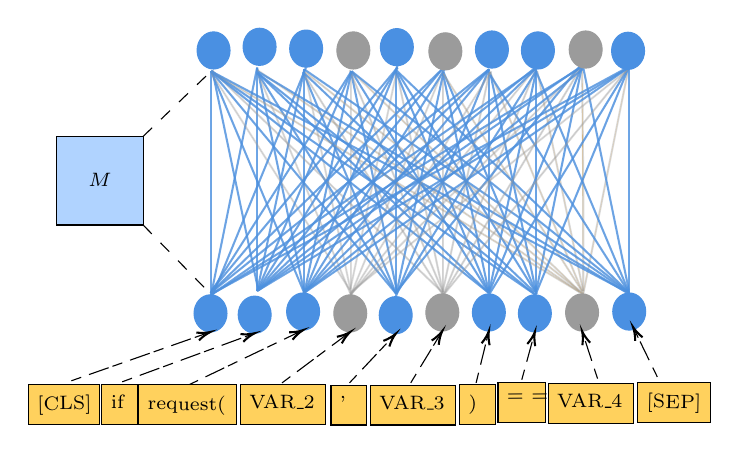
\begin{tikzpicture}[x=0.75pt,y=0.75pt,yscale=-1,xscale=1]
%uncomment if require: \path (0,428); %set diagram left start at 0, and has height of 428

%Straight Lines [id:da5087261800400087] 
\draw [color={rgb, 255:red, 74; green, 144; blue, 226 }  ,draw opacity=0.8 ][fill={rgb, 255:red, 245; green, 166; blue, 35 }  ,fill opacity=1 ][line width=0.75]    (198.82,220.29) -- (198.82,328.02) ;
%Straight Lines [id:da5857833771007241] 
\draw [color={rgb, 255:red, 74; green, 144; blue, 226 }  ,draw opacity=0.8 ][fill={rgb, 255:red, 245; green, 166; blue, 35 }  ,fill opacity=1 ][line width=0.75]    (220.99,218.53) -- (220.99,326.26) ;
%Straight Lines [id:da9472442742855178] 
\draw [color={rgb, 255:red, 74; green, 144; blue, 226 }  ,draw opacity=0.8 ][fill={rgb, 255:red, 245; green, 166; blue, 35 }  ,fill opacity=1 ][line width=0.75]    (243.71,219.41) -- (243.71,327.14) ;
%Straight Lines [id:da2204757183687085] 
\draw [color={rgb, 255:red, 155; green, 155; blue, 155 }  ,draw opacity=0.34 ][fill={rgb, 255:red, 155; green, 155; blue, 155 }  ,fill opacity=1 ][line width=0.75]    (266.16,220.29) -- (266.16,328.02) ;
%Straight Lines [id:da07267914367001382] 
\draw [color={rgb, 255:red, 74; green, 144; blue, 226 }  ,draw opacity=0.8 ][fill={rgb, 255:red, 245; green, 166; blue, 35 }  ,fill opacity=1 ][line width=0.75]    (288.04,219.85) -- (288.04,327.58) ;
%Straight Lines [id:da871368522741403] 
\draw [color={rgb, 255:red, 155; green, 155; blue, 155 }  ,draw opacity=0.39 ][fill={rgb, 255:red, 155; green, 155; blue, 155 }  ,fill opacity=1 ][line width=0.75]    (310.49,218.97) -- (310.49,326.7) ;
%Straight Lines [id:da6242406751394045] 
\draw [color={rgb, 255:red, 74; green, 144; blue, 226 }  ,draw opacity=0.81 ][fill={rgb, 255:red, 245; green, 166; blue, 35 }  ,fill opacity=1 ][line width=0.75]    (332.65,219.41) -- (332.65,327.14) ;
%Straight Lines [id:da08385924513971799] 
\draw [color={rgb, 255:red, 74; green, 144; blue, 226 }  ,draw opacity=0.81 ][fill={rgb, 255:red, 245; green, 166; blue, 35 }  ,fill opacity=1 ][line width=0.75]    (355.38,218.97) -- (355.38,275.47) -- (355.38,326.7) ;
%Straight Lines [id:da9397017332557853] 
\draw [color={rgb, 255:red, 155; green, 155; blue, 155 }  ,draw opacity=0.38 ][fill={rgb, 255:red, 245; green, 166; blue, 35 }  ,fill opacity=1 ][line width=0.75]    (377.55,217.65) -- (378.11,275.04) -- (378.11,326.26) ;
%Straight Lines [id:da11871289998091594] 
\draw [color={rgb, 255:red, 74; green, 144; blue, 226 }  ,draw opacity=0.8 ][fill={rgb, 255:red, 245; green, 166; blue, 35 }  ,fill opacity=1 ][line width=0.75]    (199.38,219.85) -- (221.55,325.82) ;
%Straight Lines [id:da41102356081521974] 
\draw [color={rgb, 255:red, 74; green, 144; blue, 226 }  ,draw opacity=0.8 ][fill={rgb, 255:red, 245; green, 166; blue, 35 }  ,fill opacity=1 ][line width=0.75]    (220.99,218.53) -- (243.71,327.14) ;
%Straight Lines [id:da2540328755628076] 
\draw [color={rgb, 255:red, 155; green, 155; blue, 155 }  ,draw opacity=0.34 ][fill={rgb, 255:red, 155; green, 155; blue, 155 }  ,fill opacity=1 ][line width=0.75]    (243.71,219.41) -- (265.88,325.39) ;
%Straight Lines [id:da08355083937039653] 
\draw [color={rgb, 255:red, 74; green, 144; blue, 226 }  ,draw opacity=0.8 ][fill={rgb, 255:red, 245; green, 166; blue, 35 }  ,fill opacity=1 ][line width=0.75]    (266.16,220.29) -- (288.32,326.26) ;
%Straight Lines [id:da9283564955752959] 
\draw [color={rgb, 255:red, 155; green, 155; blue, 155 }  ,draw opacity=0.39 ][fill={rgb, 255:red, 155; green, 155; blue, 155 }  ,fill opacity=1 ][line width=0.75]    (288.32,220.73) -- (310.49,326.7) ;
%Straight Lines [id:da867176907697975] 
\draw [color={rgb, 255:red, 74; green, 144; blue, 226 }  ,draw opacity=0.81 ][fill={rgb, 255:red, 245; green, 166; blue, 35 }  ,fill opacity=1 ][line width=0.75]    (310.49,221.17) -- (332.65,327.14) ;
%Straight Lines [id:da7853074042913364] 
\draw [color={rgb, 255:red, 74; green, 144; blue, 226 }  ,draw opacity=0.81 ][fill={rgb, 255:red, 245; green, 166; blue, 35 }  ,fill opacity=1 ][line width=0.75]    (333.22,220.73) -- (355.38,326.7) ;
%Straight Lines [id:da30815832041450086] 
\draw [color={rgb, 255:red, 155; green, 155; blue, 155 }  ,draw opacity=0.38 ][fill={rgb, 255:red, 245; green, 166; blue, 35 }  ,fill opacity=1 ][line width=0.75]    (355.94,220.29) -- (378.11,326.26) ;
%Straight Lines [id:da48960816615027136] 
\draw [color={rgb, 255:red, 74; green, 144; blue, 226 }  ,draw opacity=0.8 ][fill={rgb, 255:red, 245; green, 166; blue, 35 }  ,fill opacity=1 ][line width=0.75]    (220.99,218.53) -- (198.82,328.02) ;
%Straight Lines [id:da748254245249069] 
\draw [color={rgb, 255:red, 74; green, 144; blue, 226 }  ,draw opacity=0.8 ][fill={rgb, 255:red, 245; green, 166; blue, 35 }  ,fill opacity=1 ][line width=0.75]    (243.71,219.41) -- (220.99,326.26) ;
%Straight Lines [id:da9276037438184228] 
\draw [color={rgb, 255:red, 74; green, 144; blue, 226 }  ,draw opacity=0.8 ][fill={rgb, 255:red, 245; green, 166; blue, 35 }  ,fill opacity=1 ][line width=0.75]    (266.44,220.29) -- (243.71,327.14) ;
%Straight Lines [id:da2637766681074263] 
\draw [color={rgb, 255:red, 155; green, 155; blue, 155 }  ,draw opacity=0.34 ][fill={rgb, 255:red, 155; green, 155; blue, 155 }  ,fill opacity=1 ][line width=0.75]    (288.61,218.53) -- (265.88,325.39) ;
%Straight Lines [id:da595028187443386] 
\draw [color={rgb, 255:red, 74; green, 144; blue, 226 }  ,draw opacity=0.8 ][fill={rgb, 255:red, 245; green, 166; blue, 35 }  ,fill opacity=1 ][line width=0.75]    (310.77,220.73) -- (288.04,327.58) ;
%Straight Lines [id:da5758668522929971] 
\draw [color={rgb, 255:red, 155; green, 155; blue, 155 }  ,draw opacity=0.39 ][fill={rgb, 255:red, 155; green, 155; blue, 155 }  ,fill opacity=1 ][line width=0.75]    (332.93,220.73) -- (327.7,245.33) -- (310.21,327.58) ;
%Straight Lines [id:da3335663519598737] 
\draw [color={rgb, 255:red, 74; green, 144; blue, 226 }  ,draw opacity=0.81 ][fill={rgb, 255:red, 245; green, 166; blue, 35 }  ,fill opacity=1 ][line width=0.75]    (355.38,220.29) -- (332.65,327.14) ;
%Straight Lines [id:da1064803438688422] 
\draw [color={rgb, 255:red, 74; green, 144; blue, 226 }  ,draw opacity=0.81 ][fill={rgb, 255:red, 245; green, 166; blue, 35 }  ,fill opacity=1 ][line width=0.75]    (377.55,217.65) -- (355.38,326.7) ;
%Straight Lines [id:da20173758152649346] 
\draw [color={rgb, 255:red, 155; green, 155; blue, 155 }  ,draw opacity=0.38 ][fill={rgb, 255:red, 245; green, 166; blue, 35 }  ,fill opacity=1 ][line width=0.75]    (399.99,218.53) -- (378.11,327.58) ;
%Straight Lines [id:da45671014303975355] 
\draw [color={rgb, 255:red, 74; green, 144; blue, 226 }  ,draw opacity=0.8 ][fill={rgb, 255:red, 245; green, 166; blue, 35 }  ,fill opacity=1 ][line width=0.75]    (378.11,218.53) -- (400.13,326.04) ;
%Straight Lines [id:da4984088208739019] 
\draw [color={rgb, 255:red, 74; green, 144; blue, 226 }  ,draw opacity=0.8 ][fill={rgb, 255:red, 245; green, 166; blue, 35 }  ,fill opacity=1 ][line width=0.75]    (198.82,220.29) -- (243.71,327.14) ;
%Straight Lines [id:da13306238196157394] 
\draw [color={rgb, 255:red, 155; green, 155; blue, 155 }  ,draw opacity=0.34 ][fill={rgb, 255:red, 155; green, 155; blue, 155 }  ,fill opacity=1 ][line width=0.75]    (221.27,221.17) -- (266.16,328.02) ;
%Straight Lines [id:da4657337864585054] 
\draw [color={rgb, 255:red, 74; green, 144; blue, 226 }  ,draw opacity=0.8 ][fill={rgb, 255:red, 245; green, 166; blue, 35 }  ,fill opacity=1 ][line width=0.75]    (243.15,220.73) -- (288.04,327.58) ;
%Straight Lines [id:da47061898434255633] 
\draw [color={rgb, 255:red, 155; green, 155; blue, 155 }  ,draw opacity=0.39 ][fill={rgb, 255:red, 155; green, 155; blue, 155 }  ,fill opacity=1 ][line width=0.75]    (265.6,219.85) -- (310.49,326.7) ;
%Straight Lines [id:da10957027380370876] 
\draw [color={rgb, 255:red, 74; green, 144; blue, 226 }  ,draw opacity=0.81 ][fill={rgb, 255:red, 245; green, 166; blue, 35 }  ,fill opacity=1 ][line width=0.75]    (287.76,220.29) -- (332.65,327.14) ;
%Straight Lines [id:da1563269255921742] 
\draw [color={rgb, 255:red, 74; green, 144; blue, 226 }  ,draw opacity=0.81 ][fill={rgb, 255:red, 245; green, 166; blue, 35 }  ,fill opacity=1 ][line width=0.75]    (310.77,220.73) -- (355.66,327.58) ;
%Straight Lines [id:da4379498083520035] 
\draw [color={rgb, 255:red, 155; green, 155; blue, 155 }  ,draw opacity=0.38 ][fill={rgb, 255:red, 245; green, 166; blue, 35 }  ,fill opacity=1 ][line width=0.75]    (333.22,220.73) -- (378.11,327.58) ;
%Straight Lines [id:da609792562207087] 
\draw [color={rgb, 255:red, 74; green, 144; blue, 226 }  ,draw opacity=0.8 ][fill={rgb, 255:red, 245; green, 166; blue, 35 }  ,fill opacity=1 ][line width=0.75]    (355.38,220.29) -- (400.27,327.14) ;
%Straight Lines [id:da994309672411454] 
\draw [color={rgb, 255:red, 155; green, 155; blue, 155 }  ,draw opacity=0.34 ][fill={rgb, 255:red, 155; green, 155; blue, 155 }  ,fill opacity=1 ][line width=0.75]    (198.96,221.17) -- (266.02,326.26) ;
%Straight Lines [id:da3485360423397925] 
\draw [color={rgb, 255:red, 74; green, 144; blue, 226 }  ,draw opacity=0.8 ][fill={rgb, 255:red, 245; green, 166; blue, 35 }  ,fill opacity=1 ][line width=0.75]    (221.27,221.17) -- (288.04,327.58) ;
%Straight Lines [id:da5861115687176264] 
\draw [color={rgb, 255:red, 155; green, 155; blue, 155 }  ,draw opacity=0.39 ][fill={rgb, 255:red, 155; green, 155; blue, 155 }  ,fill opacity=1 ][line width=0.75]    (243.97,222.27) -- (310.21,327.58) ;
%Straight Lines [id:da16651104650157134] 
\draw [color={rgb, 255:red, 74; green, 144; blue, 226 }  ,draw opacity=0.81 ][fill={rgb, 255:red, 245; green, 166; blue, 35 }  ,fill opacity=1 ][line width=0.75]    (266.44,220.29) -- (332.65,327.14) ;
%Straight Lines [id:da11945946619315384] 
\draw [color={rgb, 255:red, 74; green, 144; blue, 226 }  ,draw opacity=0.81 ][fill={rgb, 255:red, 245; green, 166; blue, 35 }  ,fill opacity=1 ][line width=0.75]    (288.89,221.17) -- (355.66,327.58) ;
%Straight Lines [id:da0865328470600617] 
\draw [color={rgb, 255:red, 155; green, 155; blue, 155 }  ,draw opacity=0.38 ][fill={rgb, 255:red, 245; green, 166; blue, 35 }  ,fill opacity=1 ][line width=0.75]    (310.49,221.17) -- (377.55,326.26) ;
%Straight Lines [id:da32948653256403215] 
\draw [color={rgb, 255:red, 74; green, 144; blue, 226 }  ,draw opacity=0.8 ][fill={rgb, 255:red, 245; green, 166; blue, 35 }  ,fill opacity=1 ][line width=0.75]    (333.22,222.05) -- (400.27,327.14) ;
%Straight Lines [id:da40142239850957817] 
\draw [color={rgb, 255:red, 74; green, 144; blue, 226 }  ,draw opacity=0.8 ][fill={rgb, 255:red, 245; green, 166; blue, 35 }  ,fill opacity=1 ][line width=0.75]    (198.82,220.29) -- (288.04,327.58) ;
%Straight Lines [id:da6935916557368147] 
\draw [color={rgb, 255:red, 155; green, 155; blue, 155 }  ,draw opacity=0.39 ][fill={rgb, 255:red, 155; green, 155; blue, 155 }  ,fill opacity=1 ][line width=0.75]    (199.38,220.07) -- (310.77,327.36) ;
%Straight Lines [id:da06759068649503264] 
\draw [color={rgb, 255:red, 74; green, 144; blue, 226 }  ,draw opacity=0.81 ][fill={rgb, 255:red, 245; green, 166; blue, 35 }  ,fill opacity=1 ][line width=0.75]    (221.27,221.17) -- (332.65,327.14) ;
%Straight Lines [id:da22722871364635355] 
\draw [color={rgb, 255:red, 74; green, 144; blue, 226 }  ,draw opacity=0.81 ][fill={rgb, 255:red, 245; green, 166; blue, 35 }  ,fill opacity=1 ][line width=0.75]    (243.15,220.73) -- (354.54,326.7) ;
%Straight Lines [id:da979287841278567] 
\draw [color={rgb, 255:red, 155; green, 155; blue, 155 }  ,draw opacity=0.38 ][fill={rgb, 255:red, 245; green, 166; blue, 35 }  ,fill opacity=1 ][line width=0.75]    (266.44,220.29) -- (377.26,327.14) ;
%Straight Lines [id:da22569465328397387] 
\draw [color={rgb, 255:red, 74; green, 144; blue, 226 }  ,draw opacity=0.8 ][fill={rgb, 255:red, 245; green, 166; blue, 35 }  ,fill opacity=1 ][line width=0.75]    (288.04,219.85) -- (399.99,326.7) ;
%Straight Lines [id:da8027158903898826] 
\draw [color={rgb, 255:red, 74; green, 144; blue, 226 }  ,draw opacity=0.81 ][fill={rgb, 255:red, 245; green, 166; blue, 35 }  ,fill opacity=1 ][line width=0.75]    (198.82,220.29) -- (332.65,327.14) ;
%Straight Lines [id:da4298961957177865] 
\draw [color={rgb, 255:red, 74; green, 144; blue, 226 }  ,draw opacity=0.81 ][fill={rgb, 255:red, 245; green, 166; blue, 35 }  ,fill opacity=1 ][line width=0.75]    (221.27,221.17) -- (355.1,328.02) ;
%Straight Lines [id:da7259819631776816] 
\draw [color={rgb, 255:red, 155; green, 155; blue, 155 }  ,draw opacity=0.38 ][fill={rgb, 255:red, 245; green, 166; blue, 35 }  ,fill opacity=1 ][line width=0.75]    (244.28,220.73) -- (378.11,327.58) ;
%Straight Lines [id:da24380182183444843] 
\draw [color={rgb, 255:red, 74; green, 144; blue, 226 }  ,draw opacity=0.8 ][fill={rgb, 255:red, 245; green, 166; blue, 35 }  ,fill opacity=1 ][line width=0.75]    (266.44,220.29) -- (400.27,327.14) ;
%Straight Lines [id:da2231017046966406] 
\draw [color={rgb, 255:red, 74; green, 144; blue, 226 }  ,draw opacity=0.81 ][fill={rgb, 255:red, 245; green, 166; blue, 35 }  ,fill opacity=1 ][line width=0.75]    (198.82,220.29) -- (355.1,328.02) ;
%Straight Lines [id:da7620533427126799] 
\draw [color={rgb, 255:red, 155; green, 155; blue, 155 }  ,draw opacity=0.38 ][fill={rgb, 255:red, 245; green, 166; blue, 35 }  ,fill opacity=1 ][line width=0.75]    (221.27,219.85) -- (377.55,327.58) ;
%Straight Lines [id:da0493653969234924] 
\draw [color={rgb, 255:red, 74; green, 144; blue, 226 }  ,draw opacity=0.8 ][fill={rgb, 255:red, 245; green, 166; blue, 35 }  ,fill opacity=1 ][line width=0.75]    (243.71,219.41) -- (399.99,327.14) ;
%Straight Lines [id:da6741022333286073] 
\draw [color={rgb, 255:red, 155; green, 155; blue, 155 }  ,draw opacity=0.38 ][fill={rgb, 255:red, 245; green, 166; blue, 35 }  ,fill opacity=1 ][line width=0.75]    (198.82,220.29) -- (376.06,326.53) ;
%Straight Lines [id:da7719492193662476] 
\draw [color={rgb, 255:red, 74; green, 144; blue, 226 }  ,draw opacity=0.8 ][fill={rgb, 255:red, 245; green, 166; blue, 35 }  ,fill opacity=1 ][line width=0.75]    (221.59,220.6) -- (398.83,326.83) ;
%Straight Lines [id:da47651625468879355] 
\draw [color={rgb, 255:red, 74; green, 144; blue, 226 }  ,draw opacity=0.8 ][fill={rgb, 255:red, 245; green, 166; blue, 35 }  ,fill opacity=1 ][line width=0.75]    (198.82,220.29) -- (399.99,327.14) ;
%Straight Lines [id:da30312489810472076] 
\draw [color={rgb, 255:red, 74; green, 144; blue, 226 }  ,draw opacity=0.81 ][fill={rgb, 255:red, 245; green, 166; blue, 35 }  ,fill opacity=1 ][line width=0.75]    (399.99,218.53) -- (355.1,328.02) ;
%Straight Lines [id:da10994650807698525] 
\draw [color={rgb, 255:red, 74; green, 144; blue, 226 }  ,draw opacity=0.81 ][fill={rgb, 255:red, 245; green, 166; blue, 35 }  ,fill opacity=1 ][line width=0.75]    (377.55,217.65) -- (332.65,327.14) ;
%Straight Lines [id:da6581493587012985] 
\draw [color={rgb, 255:red, 155; green, 155; blue, 155 }  ,draw opacity=0.39 ][fill={rgb, 255:red, 155; green, 155; blue, 155 }  ,fill opacity=1 ][line width=0.75]    (355.38,218.97) -- (310.49,328.46) ;
%Straight Lines [id:da8531038082370903] 
\draw [color={rgb, 255:red, 74; green, 144; blue, 226 }  ,draw opacity=0.8 ][fill={rgb, 255:red, 245; green, 166; blue, 35 }  ,fill opacity=1 ][line width=0.75]    (332.65,219.41) -- (287.76,328.9) ;
%Straight Lines [id:da11385350638877001] 
\draw [color={rgb, 255:red, 155; green, 155; blue, 155 }  ,draw opacity=0.34 ][fill={rgb, 255:red, 155; green, 155; blue, 155 }  ,fill opacity=1 ][line width=0.75]    (311.05,218.53) -- (266.16,328.02) ;
%Straight Lines [id:da398714975138879] 
\draw [color={rgb, 255:red, 74; green, 144; blue, 226 }  ,draw opacity=0.8 ][fill={rgb, 255:red, 245; green, 166; blue, 35 }  ,fill opacity=1 ][line width=0.75]    (288.61,217.65) -- (243.71,327.14) ;
%Straight Lines [id:da26739671792084874] 
\draw [color={rgb, 255:red, 74; green, 144; blue, 226 }  ,draw opacity=0.8 ][fill={rgb, 255:red, 245; green, 166; blue, 35 }  ,fill opacity=1 ][line width=0.75]    (266.44,220.29) -- (220.99,326.26) ;
%Straight Lines [id:da42404023507655] 
\draw [color={rgb, 255:red, 74; green, 144; blue, 226 }  ,draw opacity=0.8 ][fill={rgb, 255:red, 245; green, 166; blue, 35 }  ,fill opacity=1 ][line width=0.75]    (244.61,218.35) -- (199.72,327.85) ;
%Straight Lines [id:da8828884116321025] 
\draw [color={rgb, 255:red, 74; green, 144; blue, 226 }  ,draw opacity=0.8 ][fill={rgb, 255:red, 245; green, 166; blue, 35 }  ,fill opacity=1 ][line width=0.75]    (288.61,218.53) -- (220.99,326.26) ;
%Straight Lines [id:da39259396960609383] 
\draw [color={rgb, 255:red, 74; green, 144; blue, 226 }  ,draw opacity=0.8 ][fill={rgb, 255:red, 245; green, 166; blue, 35 }  ,fill opacity=1 ][line width=0.75]    (311.33,219.41) -- (243.71,327.14) ;
%Straight Lines [id:da5471507360191554] 
\draw [color={rgb, 255:red, 155; green, 155; blue, 155 }  ,draw opacity=0.34 ][fill={rgb, 255:red, 155; green, 155; blue, 155 }  ,fill opacity=1 ][line width=0.75]    (333.78,220.29) -- (266.16,328.02) ;
%Straight Lines [id:da22668407232521326] 
\draw [color={rgb, 255:red, 74; green, 144; blue, 226 }  ,draw opacity=0.8 ][fill={rgb, 255:red, 245; green, 166; blue, 35 }  ,fill opacity=1 ][line width=0.75]    (355.66,219.85) -- (288.04,327.58) ;
%Straight Lines [id:da6161663735559477] 
\draw [color={rgb, 255:red, 155; green, 155; blue, 155 }  ,draw opacity=0.39 ][fill={rgb, 255:red, 155; green, 155; blue, 155 }  ,fill opacity=1 ][line width=0.75]    (377.55,217.65) -- (310.49,328.46) ;
%Straight Lines [id:da6009923510138324] 
\draw [color={rgb, 255:red, 74; green, 144; blue, 226 }  ,draw opacity=0.81 ][fill={rgb, 255:red, 245; green, 166; blue, 35 }  ,fill opacity=1 ][line width=0.75]    (399.99,218.53) -- (332.93,327.58) ;
%Straight Lines [id:da6906561500680035] 
\draw [color={rgb, 255:red, 74; green, 144; blue, 226 }  ,draw opacity=0.8 ][fill={rgb, 255:red, 245; green, 166; blue, 35 }  ,fill opacity=1 ][line width=0.75]    (266.44,220.29) -- (198.54,327.14) ;
%Straight Lines [id:da3966125606603381] 
\draw [color={rgb, 255:red, 155; green, 155; blue, 155 }  ,draw opacity=0.39 ][fill={rgb, 255:red, 155; green, 155; blue, 155 }  ,fill opacity=1 ][line width=0.75]    (399.99,218.53) -- (310.49,328.46) ;
%Straight Lines [id:da4205647403959616] 
\draw [color={rgb, 255:red, 74; green, 144; blue, 226 }  ,draw opacity=0.8 ][fill={rgb, 255:red, 245; green, 166; blue, 35 }  ,fill opacity=1 ][line width=0.75]    (377.83,216.33) -- (288.32,326.26) ;
%Straight Lines [id:da021488314323526714] 
\draw [color={rgb, 255:red, 155; green, 155; blue, 155 }  ,draw opacity=0.34 ][fill={rgb, 255:red, 155; green, 155; blue, 155 }  ,fill opacity=1 ][line width=0.75]    (355.66,218.09) -- (266.16,328.02) ;
%Straight Lines [id:da801391319862313] 
\draw [color={rgb, 255:red, 74; green, 144; blue, 226 }  ,draw opacity=0.8 ][fill={rgb, 255:red, 245; green, 166; blue, 35 }  ,fill opacity=1 ][line width=0.75]    (332.65,219.41) -- (243.71,327.14) ;
%Straight Lines [id:da2321169319545704] 
\draw [color={rgb, 255:red, 74; green, 144; blue, 226 }  ,draw opacity=0.8 ][fill={rgb, 255:red, 245; green, 166; blue, 35 }  ,fill opacity=1 ][line width=0.75]    (310.49,218.97) -- (220.99,326.26) ;
%Straight Lines [id:da6598597013636662] 
\draw [color={rgb, 255:red, 74; green, 144; blue, 226 }  ,draw opacity=0.8 ][fill={rgb, 255:red, 245; green, 166; blue, 35 }  ,fill opacity=1 ][line width=0.75]    (288.61,218.53) -- (199.1,325.82) ;
%Straight Lines [id:da12971361852433327] 
\draw [color={rgb, 255:red, 74; green, 144; blue, 226 }  ,draw opacity=0.8 ][fill={rgb, 255:red, 245; green, 166; blue, 35 }  ,fill opacity=1 ][line width=0.75]    (310.49,218.97) -- (198.54,327.14) ;
%Straight Lines [id:da49253940200869417] 
\draw [color={rgb, 255:red, 74; green, 144; blue, 226 }  ,draw opacity=0.8 ][fill={rgb, 255:red, 245; green, 166; blue, 35 }  ,fill opacity=1 ][line width=0.75]    (332.65,219.41) -- (221.27,326.04) ;
%Straight Lines [id:da1972642454131932] 
\draw [color={rgb, 255:red, 74; green, 144; blue, 226 }  ,draw opacity=0.8 ][fill={rgb, 255:red, 245; green, 166; blue, 35 }  ,fill opacity=1 ][line width=0.75]    (355.38,218.97) -- (243.43,327.14) ;
%Straight Lines [id:da4800861135848704] 
\draw [color={rgb, 255:red, 155; green, 155; blue, 155 }  ,draw opacity=0.34 ][fill={rgb, 255:red, 155; green, 155; blue, 155 }  ,fill opacity=1 ][line width=0.75]    (377.4,218.31) -- (265.88,327.8) ;
%Straight Lines [id:da07130484042892471] 
\draw [color={rgb, 255:red, 74; green, 144; blue, 226 }  ,draw opacity=0.8 ][fill={rgb, 255:red, 245; green, 166; blue, 35 }  ,fill opacity=1 ][line width=0.75]    (332.65,219.41) -- (198.54,327.14) ;
%Straight Lines [id:da7770285225934104] 
\draw [color={rgb, 255:red, 74; green, 144; blue, 226 }  ,draw opacity=0.8 ][fill={rgb, 255:red, 245; green, 166; blue, 35 }  ,fill opacity=1 ][line width=0.75]    (355.66,218.09) -- (221.55,325.82) ;
%Straight Lines [id:da09068033267412567] 
\draw [color={rgb, 255:red, 74; green, 144; blue, 226 }  ,draw opacity=0.8 ][fill={rgb, 255:red, 245; green, 166; blue, 35 }  ,fill opacity=1 ][line width=0.75]    (377.97,219.19) -- (243.85,326.92) ;
%Straight Lines [id:da056409582345107845] 
\draw [color={rgb, 255:red, 155; green, 155; blue, 155 }  ,draw opacity=0.34 ][fill={rgb, 255:red, 155; green, 155; blue, 155 }  ,fill opacity=1 ][line width=0.75]    (399.71,219.41) -- (296.11,302.63) -- (271.85,322.13) -- (265.6,327.14) ;
%Straight Lines [id:da20237209393358158] 
\draw [color={rgb, 255:red, 74; green, 144; blue, 226 }  ,draw opacity=0.8 ][fill={rgb, 255:red, 245; green, 166; blue, 35 }  ,fill opacity=1 ][line width=0.75]    (355.38,218.97) -- (198.82,328.02) ;
%Straight Lines [id:da7070110483341534] 
\draw [color={rgb, 255:red, 74; green, 144; blue, 226 }  ,draw opacity=0.8 ][fill={rgb, 255:red, 245; green, 166; blue, 35 }  ,fill opacity=1 ][line width=0.75]    (377.55,217.65) -- (221.55,325.82) ;
%Straight Lines [id:da05344409245075976] 
\draw [color={rgb, 255:red, 74; green, 144; blue, 226 }  ,draw opacity=0.8 ][fill={rgb, 255:red, 245; green, 166; blue, 35 }  ,fill opacity=1 ][line width=0.75]    (399.99,218.53) -- (243.85,326.92) ;
%Straight Lines [id:da6482589378215278] 
\draw [color={rgb, 255:red, 74; green, 144; blue, 226 }  ,draw opacity=0.8 ][fill={rgb, 255:red, 245; green, 166; blue, 35 }  ,fill opacity=1 ][line width=0.75]    (377.4,218.31) -- (198.82,328.02) ;
%Straight Lines [id:da30580352529745536] 
\draw [color={rgb, 255:red, 74; green, 144; blue, 226 }  ,draw opacity=0.8 ][fill={rgb, 255:red, 245; green, 166; blue, 35 }  ,fill opacity=1 ][line width=0.75]    (399.99,218.53) -- (221.55,325.82) ;
%Straight Lines [id:da9909395082271151] 
\draw [color={rgb, 255:red, 74; green, 144; blue, 226 }  ,draw opacity=0.8 ][fill={rgb, 255:red, 245; green, 166; blue, 35 }  ,fill opacity=1 ][line width=0.75]    (400.51,217.93) -- (199.34,327.42) ;
%Flowchart: Connector [id:dp15159733088575678] 
\draw  [color={rgb, 255:red, 74; green, 144; blue, 226 }  ,draw opacity=1 ][fill={rgb, 255:red, 74; green, 144; blue, 226 }  ,fill opacity=1 ] (190.6,336.97) .. controls (190.6,332.03) and (194.15,328.02) .. (198.53,328.02) .. controls (202.91,328.02) and (206.46,332.03) .. (206.46,336.97) .. controls (206.46,341.9) and (202.91,345.91) .. (198.53,345.91) .. controls (194.15,345.91) and (190.6,341.9) .. (190.6,336.97) -- cycle ;
%Flowchart: Connector [id:dp7006601580637295] 
\draw  [color={rgb, 255:red, 74; green, 144; blue, 226 }  ,draw opacity=1 ][fill={rgb, 255:red, 74; green, 144; blue, 226 }  ,fill opacity=1 ] (211.88,337.6) .. controls (211.88,332.66) and (215.43,328.66) .. (219.81,328.66) .. controls (224.19,328.66) and (227.74,332.66) .. (227.74,337.6) .. controls (227.74,342.54) and (224.19,346.55) .. (219.81,346.55) .. controls (215.43,346.55) and (211.88,342.54) .. (211.88,337.6) -- cycle ;
%Flowchart: Connector [id:dp058013988329834065] 
\draw  [color={rgb, 255:red, 74; green, 144; blue, 226 }  ,draw opacity=1 ][fill={rgb, 255:red, 74; green, 144; blue, 226 }  ,fill opacity=1 ] (235.21,336.09) .. controls (235.21,331.15) and (238.76,327.14) .. (243.14,327.14) .. controls (247.52,327.14) and (251.07,331.15) .. (251.07,336.09) .. controls (251.07,341.02) and (247.52,345.03) .. (243.14,345.03) .. controls (238.76,345.03) and (235.21,341.02) .. (235.21,336.09) -- cycle ;
%Flowchart: Connector [id:dp9687185634281383] 
\draw  [color={rgb, 255:red, 155; green, 155; blue, 155 }  ,draw opacity=1 ][fill={rgb, 255:red, 155; green, 155; blue, 155 }  ,fill opacity=1 ] (257.94,336.97) .. controls (257.94,332.03) and (261.49,328.02) .. (265.87,328.02) .. controls (270.24,328.02) and (273.79,332.03) .. (273.79,336.97) .. controls (273.79,341.9) and (270.24,345.91) .. (265.87,345.91) .. controls (261.49,345.91) and (257.94,341.9) .. (257.94,336.97) -- cycle ;
%Flowchart: Connector [id:dp18903360202066177] 
\draw  [color={rgb, 255:red, 74; green, 144; blue, 226 }  ,draw opacity=1 ][fill={rgb, 255:red, 74; green, 144; blue, 226 }  ,fill opacity=1 ] (279.83,337.85) .. controls (279.83,332.91) and (283.38,328.9) .. (287.76,328.9) .. controls (292.14,328.9) and (295.69,332.91) .. (295.69,337.85) .. controls (295.69,342.78) and (292.14,346.79) .. (287.76,346.79) .. controls (283.38,346.79) and (279.83,342.78) .. (279.83,337.85) -- cycle ;
%Flowchart: Connector [id:dp9680084215187081] 
\draw  [color={rgb, 255:red, 155; green, 155; blue, 155 }  ,draw opacity=1 ][fill={rgb, 255:red, 155; green, 155; blue, 155 }  ,fill opacity=1 ] (302.28,336.53) .. controls (302.28,331.59) and (305.83,327.58) .. (310.21,327.58) .. controls (314.59,327.58) and (318.14,331.59) .. (318.14,336.53) .. controls (318.14,341.46) and (314.59,345.47) .. (310.21,345.47) .. controls (305.83,345.47) and (302.28,341.46) .. (302.28,336.53) -- cycle ;
%Flowchart: Connector [id:dp9511999134744147] 
\draw  [color={rgb, 255:red, 74; green, 144; blue, 226 }  ,draw opacity=1 ][fill={rgb, 255:red, 74; green, 144; blue, 226 }  ,fill opacity=1 ] (324.71,336.53) .. controls (324.71,331.59) and (328.26,327.58) .. (332.64,327.58) .. controls (337.02,327.58) and (340.57,331.59) .. (340.57,336.53) .. controls (340.57,341.46) and (337.02,345.47) .. (332.64,345.47) .. controls (328.26,345.47) and (324.71,341.46) .. (324.71,336.53) -- cycle ;
%Flowchart: Connector [id:dp41134898970012146] 
\draw  [color={rgb, 255:red, 74; green, 144; blue, 226 }  ,draw opacity=1 ][fill={rgb, 255:red, 74; green, 144; blue, 226 }  ,fill opacity=1 ] (346.88,336.97) .. controls (346.88,332.03) and (350.43,328.02) .. (354.8,328.02) .. controls (359.18,328.02) and (362.73,332.03) .. (362.73,336.97) .. controls (362.73,341.9) and (359.18,345.91) .. (354.8,345.91) .. controls (350.43,345.91) and (346.88,341.9) .. (346.88,336.97) -- cycle ;
%Flowchart: Connector [id:dp46423422363247413] 
\draw  [color={rgb, 255:red, 155; green, 155; blue, 155 }  ,draw opacity=1 ][fill={rgb, 255:red, 155; green, 155; blue, 155 }  ,fill opacity=1 ] (369.62,336.53) .. controls (369.62,331.59) and (373.17,327.58) .. (377.55,327.58) .. controls (381.92,327.58) and (385.47,331.59) .. (385.47,336.53) .. controls (385.47,341.46) and (381.92,345.47) .. (377.55,345.47) .. controls (373.17,345.47) and (369.62,341.46) .. (369.62,336.53) -- cycle ;
%Flowchart: Connector [id:dp3381076199440276] 
\draw  [color={rgb, 255:red, 74; green, 144; blue, 226 }  ,draw opacity=1 ][fill={rgb, 255:red, 74; green, 144; blue, 226 }  ,fill opacity=1 ] (392.34,336.09) .. controls (392.34,331.15) and (395.89,327.14) .. (400.27,327.14) .. controls (404.65,327.14) and (408.2,331.15) .. (408.2,336.09) .. controls (408.2,341.02) and (404.65,345.03) .. (400.27,345.03) .. controls (395.89,345.03) and (392.34,341.02) .. (392.34,336.09) -- cycle ;
%Flowchart: Connector [id:dp6808063453635669] 
\draw  [color={rgb, 255:red, 74; green, 144; blue, 226 }  ,draw opacity=1 ][fill={rgb, 255:red, 74; green, 144; blue, 226 }  ,fill opacity=1 ] (192.07,210.29) .. controls (192.07,205.35) and (195.62,201.35) .. (200,201.35) .. controls (204.38,201.35) and (207.93,205.35) .. (207.93,210.29) .. controls (207.93,215.23) and (204.38,219.23) .. (200,219.23) .. controls (195.62,219.23) and (192.07,215.23) .. (192.07,210.29) -- cycle ;
%Flowchart: Connector [id:dp9998537335513744] 
\draw  [color={rgb, 255:red, 74; green, 144; blue, 226 }  ,draw opacity=1 ][fill={rgb, 255:red, 74; green, 144; blue, 226 }  ,fill opacity=1 ] (214.24,208.53) .. controls (214.24,203.59) and (217.79,199.59) .. (222.17,199.59) .. controls (226.55,199.59) and (230.1,203.59) .. (230.1,208.53) .. controls (230.1,213.47) and (226.55,217.47) .. (222.17,217.47) .. controls (217.79,217.47) and (214.24,213.47) .. (214.24,208.53) -- cycle ;
%Flowchart: Connector [id:dp6135508775164056] 
\draw  [color={rgb, 255:red, 74; green, 144; blue, 226 }  ,draw opacity=1 ][fill={rgb, 255:red, 74; green, 144; blue, 226 }  ,fill opacity=1 ] (236.68,209.41) .. controls (236.68,204.47) and (240.23,200.47) .. (244.61,200.47) .. controls (248.99,200.47) and (252.54,204.47) .. (252.54,209.41) .. controls (252.54,214.35) and (248.99,218.35) .. (244.61,218.35) .. controls (240.23,218.35) and (236.68,214.35) .. (236.68,209.41) -- cycle ;
%Flowchart: Connector [id:dp10650175513775784] 
\draw  [color={rgb, 255:red, 155; green, 155; blue, 155 }  ,draw opacity=1 ][fill={rgb, 255:red, 155; green, 155; blue, 155 }  ,fill opacity=1 ] (259.41,210.29) .. controls (259.41,205.35) and (262.96,201.35) .. (267.34,201.35) .. controls (271.72,201.35) and (275.27,205.35) .. (275.27,210.29) .. controls (275.27,215.23) and (271.72,219.23) .. (267.34,219.23) .. controls (262.96,219.23) and (259.41,215.23) .. (259.41,210.29) -- cycle ;
%Flowchart: Connector [id:dp10660584135780105] 
\draw  [color={rgb, 255:red, 74; green, 144; blue, 226 }  ,draw opacity=1 ][fill={rgb, 255:red, 74; green, 144; blue, 226 }  ,fill opacity=1 ] (280.38,208.71) .. controls (280.38,203.77) and (283.93,199.77) .. (288.31,199.77) .. controls (292.69,199.77) and (296.24,203.77) .. (296.24,208.71) .. controls (296.24,213.65) and (292.69,217.65) .. (288.31,217.65) .. controls (283.93,217.65) and (280.38,213.65) .. (280.38,208.71) -- cycle ;
%Flowchart: Connector [id:dp46759849402177966] 
\draw  [color={rgb, 255:red, 155; green, 155; blue, 155 }  ,draw opacity=1 ][fill={rgb, 255:red, 155; green, 155; blue, 155 }  ,fill opacity=1 ] (303.74,210.73) .. controls (303.74,205.79) and (307.29,201.79) .. (311.67,201.79) .. controls (316.05,201.79) and (319.6,205.79) .. (319.6,210.73) .. controls (319.6,215.67) and (316.05,219.67) .. (311.67,219.67) .. controls (307.29,219.67) and (303.74,215.67) .. (303.74,210.73) -- cycle ;
%Flowchart: Connector [id:dp8881058169733695] 
\draw  [color={rgb, 255:red, 74; green, 144; blue, 226 }  ,draw opacity=1 ][fill={rgb, 255:red, 74; green, 144; blue, 226 }  ,fill opacity=1 ] (326.19,209.85) .. controls (326.19,204.91) and (329.74,200.91) .. (334.11,200.91) .. controls (338.49,200.91) and (342.04,204.91) .. (342.04,209.85) .. controls (342.04,214.79) and (338.49,218.79) .. (334.11,218.79) .. controls (329.74,218.79) and (326.19,214.79) .. (326.19,209.85) -- cycle ;
%Flowchart: Connector [id:dp009425471783405914] 
\draw  [color={rgb, 255:red, 74; green, 144; blue, 226 }  ,draw opacity=1 ][fill={rgb, 255:red, 74; green, 144; blue, 226 }  ,fill opacity=1 ] (348.35,210.29) .. controls (348.35,205.35) and (351.9,201.35) .. (356.28,201.35) .. controls (360.66,201.35) and (364.21,205.35) .. (364.21,210.29) .. controls (364.21,215.23) and (360.66,219.23) .. (356.28,219.23) .. controls (351.9,219.23) and (348.35,215.23) .. (348.35,210.29) -- cycle ;
%Flowchart: Connector [id:dp5740386786766314] 
\draw  [color={rgb, 255:red, 155; green, 155; blue, 155 }  ,draw opacity=1 ][fill={rgb, 255:red, 155; green, 155; blue, 155 }  ,fill opacity=1 ] (371.36,209.85) .. controls (371.36,204.91) and (374.91,200.91) .. (379.29,200.91) .. controls (383.66,200.91) and (387.21,204.91) .. (387.21,209.85) .. controls (387.21,214.79) and (383.66,218.79) .. (379.29,218.79) .. controls (374.91,218.79) and (371.36,214.79) .. (371.36,209.85) -- cycle ;
%Flowchart: Connector [id:dp30959107021550936] 
\draw  [color={rgb, 255:red, 74; green, 144; blue, 226 }  ,draw opacity=1 ][fill={rgb, 255:red, 74; green, 144; blue, 226 }  ,fill opacity=1 ] (391.78,210.47) .. controls (391.78,205.53) and (395.33,201.52) .. (399.71,201.52) .. controls (404.09,201.52) and (407.64,205.53) .. (407.64,210.47) .. controls (407.64,215.41) and (404.09,219.41) .. (399.71,219.41) .. controls (395.33,219.41) and (391.78,215.41) .. (391.78,210.47) -- cycle ;
%Straight Lines [id:da05756463950883961] 
\draw  [dash pattern={on 3.75pt off 3pt on 7.5pt off 1.5pt}]  (131.5,369.44) -- (196.64,346.57) ;
\draw [shift={(198.53,345.91)}, rotate = 160.66] [color={rgb, 255:red, 0; green, 0; blue, 0 }  ][line width=0.75]    (6.56,-1.97) .. controls (4.17,-0.84) and (1.99,-0.18) .. (0,0) .. controls (1.99,0.18) and (4.17,0.84) .. (6.56,1.97)   ;
%Straight Lines [id:da3039248046479113] 
\draw  [dash pattern={on 3.75pt off 3pt on 7.5pt off 1.5pt}]  (156,369.94) -- (217.93,347.23) ;
\draw [shift={(219.81,346.55)}, rotate = 159.87] [color={rgb, 255:red, 0; green, 0; blue, 0 }  ][line width=0.75]    (6.56,-1.97) .. controls (4.17,-0.84) and (1.99,-0.18) .. (0,0) .. controls (1.99,0.18) and (4.17,0.84) .. (6.56,1.97)   ;
%Straight Lines [id:da7357894178387181] 
\draw  [dash pattern={on 3.75pt off 3pt on 7.5pt off 1.5pt}]  (188,371.44) -- (241.34,345.89) ;
\draw [shift={(243.14,345.03)}, rotate = 154.41] [color={rgb, 255:red, 0; green, 0; blue, 0 }  ][line width=0.75]    (6.56,-1.97) .. controls (4.17,-0.84) and (1.99,-0.18) .. (0,0) .. controls (1.99,0.18) and (4.17,0.84) .. (6.56,1.97)   ;
%Straight Lines [id:da07544659206674531] 
\draw  [dash pattern={on 3.75pt off 3pt on 7.5pt off 1.5pt}]  (233,370.44) -- (264.26,347.1) ;
\draw [shift={(265.87,345.91)}, rotate = 143.26] [color={rgb, 255:red, 0; green, 0; blue, 0 }  ][line width=0.75]    (6.56,-1.97) .. controls (4.17,-0.84) and (1.99,-0.18) .. (0,0) .. controls (1.99,0.18) and (4.17,0.84) .. (6.56,1.97)   ;
%Straight Lines [id:da3188945048887053] 
\draw  [dash pattern={on 3.75pt off 3pt on 7.5pt off 1.5pt}]  (265.5,370.44) -- (286.39,348.24) ;
\draw [shift={(287.76,346.79)}, rotate = 133.27] [color={rgb, 255:red, 0; green, 0; blue, 0 }  ][line width=0.75]    (6.56,-1.97) .. controls (4.17,-0.84) and (1.99,-0.18) .. (0,0) .. controls (1.99,0.18) and (4.17,0.84) .. (6.56,1.97)   ;
%Straight Lines [id:da08361117149762243] 
\draw  [dash pattern={on 3.75pt off 3pt on 7.5pt off 1.5pt}]  (295,370.44) -- (309.17,347.18) ;
\draw [shift={(310.21,345.47)}, rotate = 121.35] [color={rgb, 255:red, 0; green, 0; blue, 0 }  ][line width=0.75]    (6.56,-1.97) .. controls (4.17,-0.84) and (1.99,-0.18) .. (0,0) .. controls (1.99,0.18) and (4.17,0.84) .. (6.56,1.97)   ;
%Straight Lines [id:da022987872897272776] 
\draw  [dash pattern={on 3.75pt off 3pt on 7.5pt off 1.5pt}]  (326.5,370.44) -- (332.16,347.41) ;
\draw [shift={(332.64,345.47)}, rotate = 103.82] [color={rgb, 255:red, 0; green, 0; blue, 0 }  ][line width=0.75]    (6.56,-1.97) .. controls (4.17,-0.84) and (1.99,-0.18) .. (0,0) .. controls (1.99,0.18) and (4.17,0.84) .. (6.56,1.97)   ;
%Straight Lines [id:da35308817536672854] 
\draw  [dash pattern={on 3.75pt off 3pt on 7.5pt off 1.5pt}]  (348.5,368.94) -- (354.28,347.84) ;
\draw [shift={(354.8,345.91)}, rotate = 105.31] [color={rgb, 255:red, 0; green, 0; blue, 0 }  ][line width=0.75]    (6.56,-1.97) .. controls (4.17,-0.84) and (1.99,-0.18) .. (0,0) .. controls (1.99,0.18) and (4.17,0.84) .. (6.56,1.97)   ;
%Straight Lines [id:da9008915094337389] 
\draw  [dash pattern={on 3.75pt off 3pt on 7.5pt off 1.5pt}]  (385,368.39) -- (378.16,347.37) ;
\draw [shift={(377.55,345.47)}, rotate = 71.98] [color={rgb, 255:red, 0; green, 0; blue, 0 }  ][line width=0.75]    (6.56,-1.97) .. controls (4.17,-0.84) and (1.99,-0.18) .. (0,0) .. controls (1.99,0.18) and (4.17,0.84) .. (6.56,1.97)   ;
%Straight Lines [id:da5145832595750033] 
\draw  [dash pattern={on 4.5pt off 4.5pt}]  (166.05,251.72) -- (198.82,220.29) ;
%Straight Lines [id:da5838551448775622] 
\draw  [dash pattern={on 4.5pt off 4.5pt}]  (166.05,294.38) -- (196.6,325.59) ;
%Straight Lines [id:da41993945711340164] 
\draw [color={rgb, 255:red, 74; green, 144; blue, 226 }  ,draw opacity=0.8 ][fill={rgb, 255:red, 245; green, 166; blue, 35 }  ,fill opacity=1 ][line width=0.75]    (400.27,219.41) -- (400.27,275.91) -- (400.27,281.19) -- (400.27,327.14) ;
%Straight Lines [id:da8995804901864395] 
\draw  [dash pattern={on 3.75pt off 3pt on 7.5pt off 1.5pt}]  (413.8,367.59) -- (402.92,345.25) ;
\draw [shift={(402.05,343.45)}, rotate = 64.04] [color={rgb, 255:red, 0; green, 0; blue, 0 }  ][line width=0.75]    (6.56,-1.97) .. controls (4.17,-0.84) and (1.99,-0.18) .. (0,0) .. controls (1.99,0.18) and (4.17,0.84) .. (6.56,1.97)   ;
%Shape: Rectangle [id:dp7704156976878842] 
\draw  [fill={rgb, 255:red, 176; green, 211; blue, 255 }  ,fill opacity=1 ] (124.2,251.72) -- (166.05,251.72) -- (166.05,294.38) -- (124.2,294.38) -- cycle ;

% Text Node
\draw  [fill={rgb, 255:red, 255; green, 209; blue, 93 }  ,fill opacity=1 ]  (110.71,371.04) -- (144.89,371.04) -- (144.89,390.4) -- (110.71,390.4) -- cycle  ;
\draw (113.74,375.39) node [anchor=north west][inner sep=0.75pt]  [font=\scriptsize,rotate=-359.31] [align=left] {[CLS]};
% Text Node
\draw  [fill={rgb, 255:red, 255; green, 209; blue, 93 }  ,fill opacity=1 ]  (146.18,371.19) -- (163.35,371.19) -- (163.35,390.35) -- (146.18,390.35) -- cycle  ;
\draw (149.33,375.2) node [anchor=north west][inner sep=0.75pt]  [font=\scriptsize,rotate=-0.69] [align=left] {if};
% Text Node
\draw  [fill={rgb, 255:red, 255; green, 209; blue, 93 }  ,fill opacity=1 ]  (337.02,370.39) -- (360.14,370.39) -- (360.14,389.54) -- (337.02,389.54) -- cycle  ;
\draw (340.03,374.53) node [anchor=north west][inner sep=0.75pt]  [font=\scriptsize,rotate=-359.54] [align=left] {= =};
% Text Node
\draw  [fill={rgb, 255:red, 255; green, 209; blue, 93 }  ,fill opacity=1 ]  (256.56,371.7) -- (273.62,371.7) -- (273.62,390.75) -- (256.56,390.75) -- cycle  ;
\draw (259.61,375.71) node [anchor=north west][inner sep=0.75pt]  [font=\scriptsize,rotate=-0.22] [align=left] {,};
% Text Node
\draw  [fill={rgb, 255:red, 255; green, 209; blue, 93 }  ,fill opacity=1 ]  (163.95,371.16) -- (211.04,371.16) -- (211.04,390.44) -- (163.95,390.44) -- cycle  ;
\draw (167.03,375.17) node [anchor=north west][inner sep=0.75pt]  [font=\scriptsize,rotate=-0.37] [align=left] {request(};
% Text Node
\draw  [fill={rgb, 255:red, 255; green, 209; blue, 93 }  ,fill opacity=1 ]  (212.91,371.19) -- (254.01,371.19) -- (254.01,390.43) -- (212.91,390.43) -- cycle  ;
\draw (215.99,375.2) node [anchor=north west][inner sep=0.75pt]  [font=\scriptsize,rotate=-0.37] [align=left] {VAR\_2};
% Text Node
\draw  [fill={rgb, 255:red, 255; green, 209; blue, 93 }  ,fill opacity=1 ]  (318.33,371.12) -- (335.71,371.12) -- (335.71,390.45) -- (318.33,390.45) -- cycle  ;
\draw (321.66,375.15) node [anchor=north west][inner sep=0.75pt]  [font=\scriptsize,rotate=-1.47] [align=left] { )};
% Text Node
\draw  [fill={rgb, 255:red, 255; green, 209; blue, 93 }  ,fill opacity=1 ]  (275.63,371.68) -- (316.66,371.68) -- (316.66,390.76) -- (275.63,390.76) -- cycle  ;
\draw (278.63,375.76) node [anchor=north west][inner sep=0.75pt]  [font=\scriptsize,rotate=-359.88] [align=left] {VAR\_3};
% Text Node
\draw  [fill={rgb, 255:red, 255; green, 209; blue, 93 }  ,fill opacity=1 ]  (361.27,370.82) -- (402.3,370.82) -- (402.3,389.89) -- (361.27,389.89) -- cycle  ;
\draw (364.28,374.89) node [anchor=north west][inner sep=0.75pt]  [font=\scriptsize,rotate=-359.89] [align=left] {VAR\_4};
% Text Node
\draw  [fill={rgb, 255:red, 255; green, 209; blue, 93 }  ,fill opacity=1 ]  (404.34,370.21) -- (439.61,370.21) -- (439.61,389.75) -- (404.34,389.75) -- cycle  ;
\draw (407.57,374.22) node [anchor=north west][inner sep=0.75pt]  [font=\scriptsize,rotate=-1.02] [align=left] {[SEP]};
% Text Node
\draw (138.45,268.15) node [anchor=north west][inner sep=0.75pt]  [font=\scriptsize]  {$M$};


\end{tikzpicture}
    \caption{At every self-attention layer of each encoder block of the feature extractor, to emphasize the features that contribute to vulnerable patterns,  all attention weights related to symbolic names, which are defined in the first step of the data preprocessing phase, are filtered out. This is done by adding a mask matrix $M$ to the attention matrix $A$.
   } \label{fig:mask}
\end{figure}
\par As illustrated in Figure \ref{fig:train}, the input embedding tensor $\mathbf{X}^0$ is fed to a series of encoders. Each encoder block in the feature extractor models utilizes the multi-head self-attention mechanism, to extract the representation vector of each statement. For simplification, the formula of the self-attention layer will be formulated with a single head. Let the $\mathbf{X}_i^l$ embedding tensor be the input of the $l^{th}$ encoder block, for each $X_{ij}^l \in \mathbf{X}_i^l$ with $j\in\{1,2,3,...,n\}$, $n$ is the number of statements in the current function gadget, we have:
\begin{equation} \label{equa:FE2}
\text{MaskedAttention}(Q,K,V) = \text{Softmax}\bigg(\frac{QK^T}{\sqrt{d_k}} + \text{M}\bigg) V\end{equation}
\begin{equation} \label{equa:FE3}
A_{ij}^{l} = \text{MaskedAttention}(X_{ij}^lW_Q^l, X_{ij}^lW_K^l, X_{ij}^lW_V^l)W^l_O
\end{equation}
\begin{equation}\label{equa:FE4}
X_{ij}^{l+1} = \text{LayerNorm}(\text{MLP}( \text{LayerNorm}(A_{ij}^{l} +X_{ij}^l))+ A_{ij}^l)\end{equation}

\par The three equation \ref{equa:FE2}, \ref{equa:FE3} and \ref{equa:FE4} has three primary components: 'MaskedAttention', 'MLP', and 'LayerNorm'. The 'MLP' function is responsible for creating a fully connected feed-forward neural network, while 'LayerNorm'  use the layer normalization technique \cite{layer_norm} to normalize the layer values to ensure consistent and well-scaled data, the 'MaskedAttention' function refers to the self-attention layer that involves several sets of trainable weights denoted as $W_Q^l$, $W_K^l$, $W_V^l$, and $W_O^l$, each with a size of $d \times d$.  In order to prevent certain tokens, such as the symbolic names 'VAR\_2', 'VAR\_3', and 'VAR\_4', from being attended to by other tokens, we apply an attention mask matrix, denoted as $M$  that has the same size as the attention score matrix,  the two matrices are then added together to obtain the final attention scores. In the case of multi-head self-attention, the sizes of $W_Q^l$, $W_K^l$, and $W_V^l$ are adjusted to be $d \times (d/\text{number of heads})$ and the results of all heads from the 'MaskedAttention' function must be concatenated before multiplied by $W_O^l$.

\par In essence, the process of representation learning involves training weights that can distribute attention scores among different pairs of token embedding which determine the importance of each token in relation to the others.  Moreover, in order to ensure that the training data remains consistent, the attention signal is excluded from user-defined names and instead focused on the parts of the current statement that potentially contain vulnerable code, such as API calls, user input validation, database queries, and so on. This process allows the model  to gain a deeper understanding of the semantics of the input statements and allows the model to learn patterns in the data that are relevant to identifying potential vulnerabilities in the code base. 

\par Finally, after passing through all the layers of the encoder in the feature extractor model, the resulting embedding tensor $\mathbf{X}_i^l$ is sent through a pooling layer to extract the final representation vector for each statement. This is achieved by selecting the first token embedding of each matrix $X^l_{ij}$, indicated by the $[CLS]$ token, as the representation vector of a whole statement. Let's denote the output of the last encoder layer as $l*$, we have:
\begin{equation}\Vec{z}_{ij} = \text{CLSPooling}(X^{l*}_{ij})\end{equation}
Each embedding vector $\Vec{z}_{ij}$ is then used as an input to the classifier model, which will be discussed in the following section.

\subsubsection{Classifier} \label{sec:classifier}

\par The learning process in the classifier model follows the same pattern as that of the feature extractor. The only notable difference is that instead of using an embedding layer, we directly utilize the output representation vectors from the feature extractor.  
\begin{equation}\label{equa:cls1}
Z^0_{i}=\concat_{j=1}^{n}\Vec{z}_{ij} + PE\end{equation}
\begin{equation}\label{equa:cls2}
\text{Attention}(Q,K,V) = \text{Softmax}\bigg(\frac{QK^T}{\sqrt{d_k}}\bigg) V\end{equation}
\begin{equation}\label{equa:cls3}
A_{i}^{l} = \text{Attention}(Z_{i}^lW_Q^l, Z_{i}^lW_K^l, Z_{i}^lW_V^l)W^l_O
\end{equation}
\begin{equation}\label{equa:cls4}
Z_{i}^{l+1} = \text{LayerNorm}(\text{MLP}( \text{LayerNorm}(A_{i}^{l} +Z_{i}^l))+ A_{i}^l)\end{equation}
\par In the equation \ref{equa:cls1},  || is the concatenate operation and PE is the position embedding matrix $PE$ used to help the model understand the position of each statement in the original function. The input for the classifier model is an embedding matrix $Z^0_{i} \in \mathbb{R}^{n \times d}$ representing the embedding matrix for the function gadget $\mathbf{s}_i$. This matrix undergoes another series of encoders, similar to the feature extractor, but this time all statements are attended to without any mask, as shown in equations \ref{equa:cls2}, \ref{equa:cls3}, and \ref{equa:cls4}. Let $l*$ denote the final encoder layers we have:
\begin{equation} \label{equa:cls5} \hat{Y}_i= \text{Linear}(Z_{i}^{l*}) = W^CZ_{i}^{l*} \end{equation}
In equation \ref{equa:cls5}, $W^C$ is the learnable weights of size $d \times c$ that is used to project embeddings matrix  $Z_{i}^{l*}$ to the matrix $\hat{Y}_i \in \mathbb{R}^{n \times c}$ where $c$ is the number of classes. For each $j$ in $\{1,2,..n\}$ and $k$ in $\{0,2,..,c-1\}$, we can get the predicted labels $\mathbf{\Vec{\hat{y}}_i}$ for all statements $\mathbf{s_i}$ by choosing the class index $k$ with the highest values in each vector $\Vec{\hat{y}}_{ij} \in \hat{Y}_i$.

\begin{equation}\Vec{\hat{\mathbf{y}_{i}}} = \concat_{j=1}^{n}\argmax_k (\hat{y}_{ijk})\end{equation}


\subsubsection{End-to-end training} \label{sec:training}
In a real-world scenario, our primary objective is to pinpoint the specific code statements that are potentially suspicious and require the developer's attention for further investigation. Therefore, it is more important for a model to accurately identify all instances of vulnerable code, rather than  avoiding false positive predictions. To accomplish this, we assign weights to all statements in the dataset and use the weighted cross-entropy (WCE) loss to train the model.

Let's denote  $\theta$ as the parameters of  the deep learning model $f$. For each function gadget $\mathbf{d_i}= (\mathbf{s_i}, \Vec{y}_i)$ that have $n$ statements, the loss function is:  \begin{equation}
L_i(\theta) 
= \sum _{j=1}^{n}\frac{l_{ij}(f(s_{ij}, \theta),y_{ij})}{\sum _{i=1}^{n} w_{y_{ij}}}
= \sum _{j=1}^{n}\frac{l_{ij}(\Vec{\hat{y}}_{ij},y_{ij})}{\sum _{i=1}^{n} w_{y_{ij}}}
\end{equation}
\begin{equation}l_{ij} = w_{y_{ij}} \log \bigg ( \frac{{\exp(\hat{y}_{ij(y_{ij})}})}{\sum_{k=0}^{c-1} \exp(\hat{y}_{ijk} )}\bigg )\end{equation}
The loss function $L_i$ is defined as the weighted sum of all statement losses. To optimize the model's parameters and minimize the loss, we perform  the mini-batch stochastic gradient descent with a batch size of $n$, which also means that the model parameters are updated based on a function gadget at a time. During the training process, the adaptive gradient algorithm AdamW \cite{adamW} is used  with a linear scheduled learning rate of $1\times 10^{-5}$.
Let's $w_{y_{ij}} \in \{w_0, w_1, w_2,..,w_{c-1}\}$ denotes the weight assigned to each statement $s_{ij}$, which is calculated based on the frequency of the label $y_{ij}$ in the dataset, and the total number of samples.
\begin{equation}w_{y_{ij}}= \frac{s}{c \times s_{y_{ij}}}\end{equation}
Here, $s$ is the total number of statements of all functions gadgets in our dataset, $c$ is the number of classes, and $s_{y_{ij}}$ is the number of statements that have label $y_{ij}$.


\section{Experiments} \label{sec:experiments}
\par Throughout our experiments,  the models were trained to perform multi-class classification tasks on the entire dataset instead of separately training multiple models for binary classification with only a subset of data related to a specific CWE, as was done in a previous study by Wartschinski et al.\cite{VUDENC}. This decision was based on the fact that vulnerabilities can exist in various forms and in any part of the codebase. Therefore, training the model on a subset of data related to a specific CWE may lead to a lack of generalization,  making the model  become too "naive" and just memorizing some specific pattern from training samples. This becomes even worse when the ground truth labels themselves contain false positives samples. as a result,  apart from false negatives predictions when predicting new unseen samples, the trained models also provide many false positives because they just learned irrelevant patterns from normal code, while not actually learning anything about a vulnerable statement.  

\par By training DetectBERT on the entire dataset with diverse patterns from non-vulnerable and vulnerable statements belonging to multiple CWE, we are able to provide the model with a broader context of the codebase, which was particularly beneficial for dealing with the imbalanced dataset we had, where the number of samples in each CWE varied. Moreover, a multiclass classifier is generally more efficient in terms of cost and time for training and evaluation compared to using multiple binary classifiers for each class. This is because training multiple binary classifiers requires separate training for each one, while a multiclass classifier can be trained in a single step.


\subsection{Research questions} \label{sec:RQ}
To demonstrate the effectiveness and versatility of DetectBERT in the SVD task,  we will answer the following research questions (RQ)\\
 \textbf{RQ1}: How does adjusting hyperparameters impact the performance of DetectBERT?\\
 \textbf{RQ2}: To what extent does code normalizing and incorporating attention masks improve DetectBERT's ability to identify vulnerable code?\\
 \textbf{RQ3}: How does DetectBERT's performance in statement classification compare to baseline GNN architectures?\\
 \textbf{RQ4}: What are the statement types in which DetectBERT performs particularly well?\\

 \begin{table*}[h]
\centering
\begin{tabular}{lllllllllll}
\toprule
\Xhline{2\arrayrulewidth}
\textbf{Dataset} & \textbf{Normal} & \textbf{CWE-22} & \textbf{CWE-77} & \textbf{CWE-79} & \textbf{CWE-89} & \textbf{CWE-352} & \textbf{CWE-601} & \textbf{CWE-94} & \textbf{ \makecell{Total number  of \\ function gadgets }}
& \textbf{\makecell{Total number\\ of statements}}\\
\midrule
\hline
CVEFixes & 5301 & 68 & n/a & 102 & n/a & 40& 150 & 69 & 15841 & 153919\\
VUDENC & 13020 &325 & 328 & 58 & 1123 & 526& 246& 215 & 5730 & 57398\\
\Xhline{2\arrayrulewidth}
\bottomrule
\end{tabular}
\label{table:data_stat}
\caption{The statistics about the number of function gadgets ($d_i$) containing vulnerable patterns specific to each CWE type. The final two columns present the total number of function gadgets in $d_i$, along with the total number of statements ($s_{ij}$) for both datasets VUDENC and CVEFixes.}
\end{table*}
\subsection{Metrics for evaluation}\label{sec:metrics}

\par Since the vulnerable code often accounts for a small portion of the code base, the dataset for vulnerable code detection always results in heavy imbalance distribution. So to evaluate the classification model, the F1 score, precision, and recall were used as metrics to evaluate the performance of the methods used for detecting vulnerable code, which is a common practice in many studies related to this topic \cite{Linevd,MVD}. All of these metrics rely on four main statistical components that are: true positive (TP), true negative (TN), false positive (FP), and false negative (FN). 
\begin{equation}\label{equa:metric1}Precision= \frac{TP}{TP+FP}\end{equation}
\begin{equation}\label{equa:metric2}Recall=\frac{TP}{TP+FN}\end{equation}
\begin{equation}\label{equa:metric3}F1=\frac{2 \times Precision \times Recall}{Precision + Recall}\end{equation}
\par The formulas above are used in the case of binary classification.  However, since our model is used for multi-label classification problems and the distribution between ground truth labels is also not balanced, we employ the macro-F1, macro-precision, and macro-recall to handle this. 

\begin{equation}\label{equa:metric4}Precision_{macro}= \frac{1}{c} \sum _{i=0}^{c-1}\frac{TP_i}{TP_i+FP_i}\end{equation}
\begin{equation}\label{equa:metric5}Recall_{macro}= \frac{1}{c} \sum _{i=0}^{c-1}\frac{TP_i}{TP_i+FN_i}\end{equation}
\begin{equation}\label{equa:metric6}
F1_{marcro}=\frac{2 \times Precision_{macro} \times Recall_{marco}}{Precision_{macro} + Recall_{macro}}
\end{equation}

\par In the case of vulnerable code detection, recall measures the fraction of correctly detected vulnerable statements out of all statements that contain vulnerable code, while precision represents the fraction of accurately predicted results among all predicted results. The macro-versions of these metrics aggregate the results across all labels, treating each label equally, which is crucial for imbalanced multi-label classification problems. 
\par Another metric that was used in our experiment is  the  Area Under the Curve (AUC) score of the Receiver Operating Characteristic (ROC) curve (AUROC). This metric  is frequently utilized to evaluate the performance of a classification model.  While the ROC curve illustrates the balance between the TP rate (sensitivity) and FP rate (1-specificity) for different threshold values, the AUROC score indicates the degree of separability between positive and negative samples in the classification task by calculating the area under the ROC curve that range from 0 to 1. A score of 1 indicates perfect separability, while a score of 0.5 indicates random guessing. In our use case,  The AUROC score can be used to determine the model's ability to confidently distinguish between vulnerable and non-vulnerable code based on the predicted probabilities.  In mathematical terms, the formula for AUROC can be written as:
\begin{equation} \label{equa:TPR}
  \mathrm{sensitivity}= Recall =  TPR = \frac{TP}{TP + FN} 
\end{equation}
\begin{equation}\label{equa:FPR}
    1 - \mathrm{specificity} = FPR = \frac{TP}{TN + FP}
\end{equation}
\begin{equation} \label{equa:metric7}
AUROC = \int_{0}^{1} TPR(FPR) \ dFPR
\end{equation}
\begin{equation} \label{equa:metric8}
    \mathrm{AUROC}_{macro} = \frac{\sum_{i=0}^{c-1} \mathrm{AUROC}_i}{c}
\end{equation}

\par The $TPR(FPR)$ function in equation \ref{equa:metric7}   represent the formula for TPR as a function of FPR depending on the specific classification model being used.  The results of the $TPR(FPR)$ function describe the trade-off between TPR and FPR at various classification thresholds and are typically plotted as the ROC curve. The AUROC is then calculated as the area under this curve. Finally, the $\mathrm{AUROC}_{macro}$ score is calculated in equation \ref{equa:metric8} to represent the confidence of the model the calculate a sample with ground truth label $i \in \{0,1,...,c-1\}$ as $i$ .

\par While the metrics discussed earlier are helpful for evaluating the performance of a model, as mentioned  in the section \ref{sec:I}, it's worth noting that the ground truth labels themselves may not be entirely accurate, and may contain false positives. Therefore, to better analyze the agreement of the models to the provided ground truth label for each type of statement,  the Matthews correlation coefficient (MCC) is  used combined with F1. While F1 is independent of TN predictions, MCC takes into account all four categories of statistical components.
 \begin{equation}\label{equa:mcc}MCC=\frac{
 TP\times TN - FP \times FN
 }
 {
 \sqrt{(TP+FP)(TP+FN)(TN+FP)(TN+FN)}
 }\end{equation}
 \begin{equation} \label{equa:mcc_macro}
    \mathrm{MCC}_{macro} = \frac{\sum_{i=0}^{c-1} \mathrm{MCC}_i}{c}
\end{equation}
 \par In equation \ref{equa:mcc}, the MCC formula produces an output value between -1 and 1, and the equation \ref{equa:mcc_macro} shows the macro average formula for the MCC score of all classes $i\in \{0, 1, 2, ..., c - 1\}$ . When the MCC has a value of 1, it indicates that the model's predictions align perfectly with the provided ground truth labels, otherwise a 0 score indicates a random prediction, and -1 indicates a completely wrong prediction.

\subsection{Datasets} 

\par The VUDENC dataset \cite{VUDENC} is a useful resource for studying code commits that address issues related to  specific Common Weakness Enumerations (CWEs) in open-source repositories. However, the primary limitation of this dataset is the existence of a substantial number of duplicated samples. This leads to severe data leakage problems between the train and test sets, resulting in over-optimistic experimental results. There are three main factors contributing to this issue. Firstly, the preprocessing approach used in VUDENC involves tokenizing all code in a Python file and extracting a slice of code with a fixed window size of $m$ tokens for every $n$ tokens step (in VUDENC $m=200$ and $n=5$). This method generates a large number of overlapping slices, exacerbating the problem of duplicated samples. Secondly, all the data in VUDENC comes from commits that are used to fix Github issues with tags and descriptions related to specific CWEs. Therefore, there might be instances where the same file is fixed multiple times, leading to additional duplicated code slice samples. Lastly, code reuse in open-source projects also contributes to the duplication issue in the VUDENC dataset. To reduce the duplicated sample, the data preprocessing pipeline mentioned in section \ref{sec:FE}  was applied to create a new version of the VUDENC dataset.  

\par To better evaluate DetectBERT's performance, we also used the publicly available CVEFixes dataset in addition to the VUDENC dataset. This ensures the model's effectiveness and reliability in practical settings, thereby contributing to the improvement of security across multiple projects. The CVEFixes dataset was created by collecting Common Vulnerabilities and Exposures (CVE) records from the National Vulnerability Database (NVD) and identifying the relevant GitHub commits that address the vulnerabilities via the attached URLs that are linked to the patching commits. Only records used to patch vulnerabilities in Python were selected by applying a filter to the dataset, which is then further processed to include only the CVE records related to the CWE categories in the VUDENC dataset. The same preprocessing steps are applied to the CVEFixes dataset as well.


\par Table \ref{table:data_stat} provides a detailed overview of our processed datasets, including the number of samples for each CWE. The CWEs that are included in our datasets are: 
\begin{itemize}
    \item CWE-22\cite{cwe22}: Improper Validation of Input Data. This is a type of vulnerability that arises when input data from external sources is not properly validated before being used by the software, which can lead to various security issues.
    \item CWE-79\cite{cwe79}: Improper Neutralization of Input During Web Page Generation. This is a vulnerability in web applications that occurs when untrusted user input is not properly sanitized or escaped, which can allow an attacker to inject malicious code into the web page and perform actions on behalf of the victim.
    \item CWE-77\cite{CWE-77}: Improper Neutralization of Special Elements used in a Command ('Command Injection'). This vulnerability occurs when untrusted user input is passed to a command shell or other interpreter as part of a command, which can allow an attacker to execute arbitrary code or commands on the system.
    \item CWE-89\cite{CWE-89}:  Improper Neutralization of Special Elements used in an SQL Command ('SQL Injection'). This vulnerability occurs when untrusted user input is not properly sanitized before being used in an SQL query, which can allow an attacker to inject malicious SQL code and access or modify sensitive data.
    \item CWE-94\cite{cwe94}:  Improper Control of Generation of Code ('Code Injection'). This is a type of vulnerability that occurs when untrusted user input is used to generate executable code, which can allow an attacker to inject and execute arbitrary code on the system.
    \item     CWE-352\cite{cwe352}: Cross-Site Request Forgery (CSRF). This vulnerability occurs when an attacker is able to trick a victim into performing an action on a website or application that the victim did not intend to perform, by exploiting the victim's existing authenticated session on that site.
    \item     CWE-601\cite{cwe601}:  URL Redirection to Untrusted Site ('Open Redirect'). This is a vulnerability that occurs when a web application redirects a user to an untrusted or malicious site, which can be exploited by an attacker to steal sensitive information or perform other malicious actions.
\end{itemize}

\par The datasets were divided into training and testing sets with a ratio of $80:20$. Given that the number of samples in each class varied, with some classes having only a small number of samples, during the evaluation phase, the k-Fold cross-validation technique with $k=5$  was used to ensure that our model was adequately validated and produced robust results.



\subsection{Pretrained feature extractors}\label{sec:feature_extractors}
\begin{table}[h]
\centering
\begin{tabular}{lcccc}
\Xhline{2\arrayrulewidth}
\textbf{\makecell{Feature\\ extractor}} & \textbf{\makecell{Num\\ layers}} & \textbf{Hidden size} &  \textbf{Pooling} & \textbf{Model size} \\
 \hline
 MiniLM\cite{minilm} &  12  & 384 &  CLS pooling & 120 MB\\
 mpnet\cite{mpnet} & 12 & 768 &  CLS pooling & 420 MB\\
\Xhline{2\arrayrulewidth}
\end{tabular}
\caption{Throughout our experiments, we utilized two models - MiniLM and mpnet - for extracting embedding vectors from Python statements and evaluated their impact on the performance of the models. }
\label{table:Embedding}
\end{table}
In our Python vulnerability detection experiments, two different embedding models, mpnet and MiniLM, are  utilized as feature extractors for our DetectBERT models. The mpnet has a hidden size of 768, while MiniLM has a hidden size of 384. Both models were pre-trained using contrastive learning objective \cite{sbert} on a massive corpus of over one billion sentence pairs, consisting of both natural languages and code. The training corpus for code included pairs from multiple programming languages, such as Python, Javascript, Ruby, Go, Java, and PHP, which were obtained from the CodeSearchNet dataset\cite{husain_codesearchnet_2019}. Table \ref{table:Embedding} provides additional information about these feature extractors such as the number of encoder layers, the pooling strategy, and the model size.
\subsection{Experiment results}
This section offers  information about how each experiment was conducted for each of the research questions (RQ) outlined in section \ref{sec:RQ}. It includes details on the selection and preparation of the data and models, as well as the empirical results obtained.  Also, insights regarding  results are also discussed to answer those RQs. 
\subsubsection{Experiment results for RQ1}
\begin{table}[h]
\centering
\begin{tabular}{cccccc}
\toprule
\Xhline{2\arrayrulewidth}
\textbf{\makecell{Hidden\\ size}} & \textbf{\makecell{Num \\ heads} }& \textbf{\makecell{Num \\ layers}} & \textbf{\makecell{F1 score\\ (F1)}} & \textbf{\makecell{Precision\\ (Prec)}} & \textbf{\makecell{Recall\\ (Rec)}}\\
\midrule
\hline
\multirow{20}{*}{$h_{MiniLM}=384$}     & \multirow{4}{*}{2}  
         & 3  &62.86 & 56.38 &72.26\\
    &    &\rowcolor{gray!15}  6  &64.23 & 58.74 &73.41 \\
    &    & 9  &57.58 & 48.77 &75.84  \\
    &    &\rowcolor{gray!15}  12 &57.31 & 49.55 &73.52 \\
\cline{2-6}
    & \multirow{4}{*}{4}  & 3  &67.07 & 64.89 &71.27  \\
    &    &\rowcolor{gray!15}  6  &65.54 & 58.46 & \textbf{76.26}  \\
    &    & 9  &49.70 & 42.50 &74.11 \\
    &    &\rowcolor{gray!15}  12 &64.70 & 61.59 &70.21  \\
\cline{2-6}
    & \multirow{4}{*}{6}  & 3  &70.71 & 67.12 &75.54 \\
    &    &\rowcolor{gray!15}  6  &57.58 & 49.19 &73.99 \\
    &    & 9  &61.85 & 53.86 &74.90 \\
    &    &\rowcolor{gray!15}  12 &65.65 & 62.55 &70.43\\
\cline{2-6}
    & \multirow{4}{*}{12} & 3  &\textbf{71.33} & \textbf{71.10} &73.40  \\
    &    &\rowcolor{gray!15}  6  &57.13 & 50.17 &70.26  \\
    &    & 9  &66.10 & 63.84 &70.87\\
    &    &\rowcolor{gray!15}  12 &60.92 & 53.12 &73.96\\
\cline{2-6}
    & \multirow{4}{*}{24} & 3  &62.75 & 57.96 &71.22 \\
    &    &\rowcolor{gray!15}  6  &63.43 & 55.45 &76.15\\
    &    & 9  &62.05 & 54.28 &74.87\\
    &    &\rowcolor{gray!15}  12 &56.14 & 47.85 &71.64\\
\hline
\multirow{20}{*}{$h_{mpnet}=768$} 
    & \multirow{4}{*}{2} & 3  &71.07 & 69.50 &74.90\\
    &    &\rowcolor{gray!15}  6  &69.37 & 65.56 &74.70 \\
    &    & 9  &65.54 & 63.80 &70.28 \\
    &    &\rowcolor{gray!15}  12 &64.18 & 59.39 &74.21 \\
\cline{2-6}
    & \multirow{4}{*}{4}  & 3  &\textbf{74.47} & \textbf{77.10} &72.39\\
    &    &\rowcolor{gray!15}  6  &70.60 & 66.77 &75.42\\
    &    & 9  &64.93 & 59.38 &73.35\\
    &    &\rowcolor{gray!15}  12 &63.02 & 58.72 &72.06\\
\cline{2-6}    
    & \multirow{4}{*}{6}  & 3  &63.98 & 56.23 &\textbf{77.85}\\
    &    &\rowcolor{gray!15}  6  &68.54 & 65.22 &73.93 \\
    &    & 9  &63.57 & 58.64 &74.21 \\
    &    &\rowcolor{gray!15}  12 &59.64 & 66.28 &63.05 \\
\cline{2-6}    
    & \multirow{4}{*}{12} & 3  &72.27 & 73.00 &72.15\\
    &    &\rowcolor{gray!15}  6  &71.96 & 69.16 &76.47\\
    &    & 9  &60.56 & 54.05 &71.60\\
    &    &\rowcolor{gray!15}  12 &69.31 & 69.06 &71.62\\
\cline{2-6}
    & \multirow{4}{*}{24} & 3  &72.37 & 69.69 &76.47\\
    &    &\rowcolor{gray!15}  6  &69.26 & 65.36 &74.07\\
    &    & 9  &63.66 & 59.39 &70.37\\
    &    &\rowcolor{gray!15}  12 &72.22 & 75.11 &69.96\\
\Xhline{2\arrayrulewidth}
\bottomrule
\end{tabular}
\label{table:hyperparam_result}

\caption{The experiment involved training multiple models on a combined dataset comprising samples from processed VUDENC and CVEfixes, each with its own set of hyperparameters. These models were trained using the training strategy discussed in section \ref{sec:training} for a duration of 100 epochs. The experimental results showed that the models with the best performance had larger hidden sizes, such as $h_{mpnet}=768$, and had three classifier layers. }
\end{table}
\par \textbf{Data and model preparation}: To explore how hyperparameters can influence the performance of machine learning models, it is often necessary to experiment with various hyperparameter configurations. In our study, we attempted to optimize the DetectBERT model's hyperparameters by adjusting the hidden size, number of encoders, and number of attention heads in the classifier model. To be more efficient in terms of both cost and time,  the VUDENC and CVEfixes datasets were merged for training and evaluation. This was also necessary, since as shown in table \ref{table:data_stat}, the CVEfixes dataset contained a limited number of samples related to classes CWE-89 and CWE-77.  All the models are trained for 100 epochs using the training strategy discussed in section \ref{sec:training}.

\begin{figure*}[h]
    \centering
    \includesvg[width=\textwidth, align=center]{RQ2_H.svg}
    \includesvg[width=\textwidth, align=center]{RQ2_Head.svg}
    \caption{Plots that are created to illustrate how DetectBERT performs on three metrics - F1, precision, and recall  scores - with different parameters. The red lines in the plots represent models with hidden sizes of 384, while the blue lines represent models with hidden sizes of 768.}
 \label{fig:RQ1_graphs}
\end{figure*}


\par \textbf{Experiment results}: Detailed breakdown of the observed results can be found in table \ref{table:hyperparam_result}, we have also created a series of subplots in figure \ref{fig:RQ1_graphs} to help visualize how the different hyperparameters were correlated to the performance of the model.
\par From the results in Figure \ref{fig:RQ1_graphs}, it is noticeable that larger hidden sizes in models generally lead to better performance in all metrics. Specifically,  when comparing models with hidden size $h=384$ to those with $h=768$,  the smaller models achieved competitive recall scores ranging from 69.96\% to 77.85\%,  However, given the same set of other hyperparameters (number of classifier layers and attention heads), the larger models consistently achieved better precision scores of 54\% to 77\% compared to smaller models, which ranged from 42\% to 71\%. Consequently, the larger models also achieved better F1 scores ranging from 59\% to 74\%, while smaller models with hidden size ($h=384$) only achieved F1 scores ranging from 49\% to 71\%. Overall, these results align with previous studies such as \cite{attention, bert} which suggest that larger hidden sizes enable models to capture more complex features, thus improving their ability to generalize to new data. 

\par Another pattern  that can be observed is that the number of encoder layers in the classifier model did not have a significant impact on the performance of DetectBERT. In fact, models with fewer classifier layers tended to perform better. One possible explanation for this observation is the risk of overfitting. When the number of encoder layers is high, the model may become too specialized for the training data, resulting in poor generalization performance on new data. Therefore, using fewer classifier layers might provide a better balance between model complexity and generalization ability. To prove this point, we also provide details about how DetectBERT work behind the scene in appendix \ref{sec:behind_the_scene}

\par Regarding the number of attention heads, our empirical results suggest that having more  many attention heads does not necessarily imply any improvement in the final performance. In reality, too many attention heads could cause the hidden size to be divided into very small sub-dimensions leading to missing necessary features for each head. The most stable and optimal number of attention heads was found to be 12  for  both $h=384$ and 24 for $h=768$.

\par In conclusion, for optimal performance in our study, a model with a larger hidden size of $h_{mpnet}=768$ for both the feature extractor and classifier is suggested. While models with 6 classifier layers can be considered, we recommend using a model with only 3 classifier layers as we have observed more stable performance during the training phase with such models. And as suggested for $h_{mpnet}=768$, the ideal number of attention heads is $24$. 
\begin{table*}[h]
\centering
\begin{tabular}{|c|c|c|lcccccccc|}
\toprule

\Xhline{2\arrayrulewidth}

\textbf{\makecell{Evaluate\\scenarios}} & \textbf{Dataset} & \textbf{\makecell{Normalized }} & \textbf{Metric} & \textbf{CWE-22} & \textbf{CWE-77} & \textbf{CWE-79} & \textbf{CWE-89} & \textbf{CWE-352} & \textbf{CWE-601} & \textbf{CWE-94}&\textbf{Average}\\
\midrule
\hline


\multirow{16}{*}{Normal}
&\multirow{8}{*}{CVEFixes}
&\multirow{4}{*}{False}
 
&     F1 &\textbf{51.61}& n/a &53.66& n/a &80.95&72.09& \textbf{90.41} & 69.74\\

&&    &\rowcolor{gray!15} Prec&\textbf{61.54}& n/a &\textbf{91.67}& n/a &85.00&81.58& \textbf{94.29} &\textbf{82.82}\\
&&    &Rec&44.44& n/a &37.93& n/a &77.27&64.58& 86.84&62.15\\
&&    &\rowcolor{gray!15}  AUROC &63.74& n/a &\textbf{77.71}& n/a &\textbf{98.69}&90.79& 95.65 & 85.30\\
\cline{3-12}
&&\multirow{4}{*}{True}

    &     F1 & 42.30& n/a &\textbf{54.55}& n/a &\textbf{93.02}&\textbf{75.48}& 86.19&\textbf{70.30}\\

&&&\rowcolor{gray!15} Prec&36.36& n/a &57.69& n/a &\textbf{95.24}&\textbf{88.57}& 82.50 &72.67\\
 
&&&Rec&\textbf{50.56}& n/a &\textbf{51.72}& n/a &\textbf{90.91}&\textbf{65.76}& \textbf{90.23}&\textbf{69.83}\\

&&&\rowcolor{gray!15}  AUROC&\textbf{80.12}& n/a &77.42& n/a &97.81&\textbf{94.43}& \textbf{99.64}&\textbf{89.88}\\
    \cline{2-12}


&\multirow{8}{*}{VUDENC}
&\multirow{4}{*}{False}
&     F1 &\textbf{63.42}&\textbf{66.67}&\textbf{42.90}&\textbf{64.88}&\textbf{72.38}&\textbf{73.25}& \textbf{78.79}&\textbf{66.04}\\

&&    &\rowcolor{gray!15}   Prec&\textbf{52.82}&\textbf{73.50}&\textbf{40.09}&\textbf{67.80}&\textbf{66.20}&\textbf{65.44}& \textbf{77.38}&\textbf{63.30}\\

&&    &Rec&79.37&60.99&46.15&62.20&79.83&\textbf{83.18}& 80.25&70.28\\
  
&&    &\rowcolor{gray!15}    AUROC &\textbf{92.38}&\textbf{92.77}&\textbf{84.72}&86.43&93.51&96.27& 89.94&90.86\\
\cline{3-12}
&&\multirow{4}{*}{True}
&     F1 &50.41&64.23&39.75&51.37&60.78&48.75& 66.33&54.52\\   
   
&&    &\rowcolor{gray!15}   Prec&36.60&66.17&33.33&42.41&47.21&34.72& 55.93&45.19\\   

&&    &Rec&\textbf{80.95}&\textbf{62.41}&\textbf{49.22}&\textbf{65.14}&\textbf{85.29}&81.78& \textbf{81.48}&\textbf{72.32}\\

&&    &\rowcolor{gray!15}    AUROC&91.59&88.30&79.64&\textbf{88.68}&\textbf{95.76}&\textbf{97.35}& \textbf{94.13}&\textbf{91.77}\\
\hline

\multirow{16}{*}{Augmented}
&\multirow{8}{*}{CVEFixes}
&\multirow{4}{*}{False}
&     F1 &23.08 & n/a & \textbf{27.03}& n/a & 58.82& 69.23& 67.80&49.20\\

&&    &\rowcolor{gray!15}   Prec&\textbf{37.50} & n/a & \textbf{62.50} & n/a & 83.33& \textbf{90.00}& \textbf{95.24}&\textbf{73.71} \\

&&    &Rec&16.67 & n/a & 17.24& n/a & 45.45& 56.25& 52.63&37.64\\
 
&&    &\rowcolor{gray!15}    AUROC &\textbf{64.36} & n/a & 68.09& n/a & \textbf{99.04}& 90.50& 97.53&82.70\\
\cline{3-12}

&&\multirow{4}{*}{True}
&     F1 &\textbf{30.30}& n/a & 24.00& n/a & \textbf{74.29}& \textbf{73.81}& \textbf{77.92}&\textbf{56.06}\\

&&    &\rowcolor{gray!15}   Prec&33.33& n/a & 28.57& n/a & \textbf{100.00}& 86.11& 76.92&64.99\\
  
&&    &Rec&\textbf{27.78}& n/a & \textbf{20.69}& n/a & \textbf{59.09}& \textbf{64.58}& \textbf{78.95}&\textbf{50.22}\\

&&    &\rowcolor{gray!15}    AUROC &63.89& n/a & \textbf{74.46}& n/a & 98.62& \textbf{94.34}& \textbf{99.04}&\textbf{86.07}\\ 
\cline{2-12}

&\multirow{8}{*}{VUDENC}
&\multirow{4}{*}{False}

&     F1 &48.48& \textbf{48.11}& \textbf{45.45}& \textbf{45.45}& \textbf{71.16}& \textbf{48.33}& \textbf{50.82}&\textbf{51.11}\\
 
&&    &\rowcolor{gray!15}   Prec&\textbf{66.67}& \textbf{71.83}& \textbf{55.56}& \textbf{62.30}& \textbf{71.31}& \textbf{59.59}& \textbf{75.61}&\textbf{66.12}\\  

&&    &Rec&38.10& 36.17& 38.46& 35.78& 71.01& 40.65& 38.27&42.63\\

&&    &\rowcolor{gray!15}    AUROC &90.76& 82.94& 76.28& 78.89& 94.54& 91.55& 85.77&85.81\\
\cline{3-12}

&&\multirow{4}{*}{True}
&    F1 &\textbf{53.41}& 45.85& 29.41& 43.97& 50.97& 42.58& 50.22&45.19\\
  
&&    &\rowcolor{gray!15}   Prec&41.59& 51.79& 23.81& 38.54& 36.82& 31.35& 39.44&37.62\\
  
&&    &Rec&\textbf{74.60}& \textbf{41.13}& \textbf{38.46}& \textbf{51.19}& \textbf{82.77}& \textbf{66.36}& \textbf{69.14}&\textbf{60.52}\\

&&    &\rowcolor{gray!15}    AUROC&\textbf{91.51}& \textbf{89.24}& \textbf{78.43}& \textbf{88.69}& \textbf{96.53}& \textbf{97.02}& \textbf{91.78}&\textbf{90.45}\\
\Xhline{2\arrayrulewidth}

\bottomrule
\end{tabular}
\label{table:RQ2_result}
\caption{The table presents the outcomes of the DetectBERT models in experiments for RQ2, in both normalized and unnormalized versions of the two datasets - VUDENC and CVEFixes. The empirical  data contains the models' performance on various metrics, such as f1, precision, recall, and AUROC score, in two evaluation scenarios, which are the standard test set and augmented test sets, where random strings substituted user-defined names like variable and method names. }
\end{table*}
\subsubsection{Experiment results for RQ2}


\par This section will discuss the data and the experiment results that are conducted to assess the contribution  of the code normalization steps and the attention mask $M$, which are introduced in sections \ref{sec:FE} and \ref{sec:ME} respectively,  to the performance of DetectBERT. 
\par \textbf{Data preparation}:  Experiments are conducted separately with two versions of each dataset - VUDENC and CVEFixes. The first version contained unprocessed function gadgets with the original code, while the second version replaced all inconsistencies such as user-defined variable names, method names, and class names with symbolic names like 'VAR\_1' and 'FUNC\_3'. The models used in this experiment are then trained on both versions of the datasets and evaluated in two scenarios:
\begin{itemize}
    \item In the first scenario, we split the data into a train and test set with an 80:20 ratio. The model is then trained using the train and evaluation splits respectively.
    \item In the second scenario,  the datasets are also split into train and test sets with the same ratio, but the test set is augmented by replacing all user-defined variables and method names with random strings such as 'a', 'b', 'c', etc. This was done to evaluate the robustness of the model against adversarial attacks where the same vulnerable pattern may be disguised by features that are not relevant to the vulnerable pattern.
\end{itemize}
\par In this experiment,  the two datasets CVEfixes, and VUDENC were not concatenated like in RQ1, as we wanted to evaluate the consistency of the model's performance across different data distributions. Both scenarios utilized k-fold cross-validation for a more accurate evaluation.
\par \textbf{Models preparation}: As demonstrated in the previous analysis for RQ1, the performance of the model improves as the hidden size of the model increases. Therefore, in this experiment, the pre-trained mpnet model was chosen as the feature extractor and a classifier that contains 3 layers of transformer encoders was also employed. To assess the effectiveness of the attention mask $M$ combined with code normalization, a different feature extraction approach was used depending on whether the dataset was normalized or unnormalized. Specifically, as discussed in section \ref{sec:MFE} for processed datasets,  an attention mask was applied to eliminate the attention signal generated by the symbolic names. Our hypothesis is that this approach can enable the model  to focus more effectively on the actual vulnerable patterns, and identify the relevant features that are important for the classification task. On the other hand, for unprocessed datasets, the standard self-attention layer was used for feature extraction.

\par \textbf{Results}: Table \ref{table:RQ2_result} provides a detailed description of the results obtained from our experiment. A trade-off between precision and recall was observed when training the model on normalized and unnormalized datasets in both scenarios. 
\par Particularly, our empirical results showed that models trained on normalized datasets outperformed models trained on unnormalized datasets in terms of recall  scores in both scenarios. In the normal scenario, models trained on normalized code achieved an average recall score of 69.83\% for CVEfixes and 72.32\% for VUDENC, while models trained on the original code had slightly lower recall scores, with 62.15\% for CVEFixes and 70.28\% for VUDENC. The difference in the recall scores of the models trained on normalized and unnormalized data was even more significant in the second scenario, with models trained on unnormalized data achieving significantly lower recall scores (37.64\% for CVEFixes and 42.63\% for VUDENC), while the recall scores for models trained on normalized code were less affected (50.22\% for CVEFixes and 60.52\% for VUDENC).

\par In contrast, models trained on unnormalized data had better precision than those trained on normalized data, except for CWE types such as CWE-352 and CWE-601 in the CVEfixes dataset. Specifically, the average precision score for models trained on unnormalized code was 82.82\% for CVEFixes and 63.30\% for VUDENC, outperforming models trained on normalized code, which achieved a precision score of 72.67\% for CVEFixes and 45.19\% for VUDENC. The same pattern was observed in the second scenario, where the precision scores dropped for both normalized and unnormalized models, but the precision scores of models trained on unnormalized data (73.71\% for CVEFixes and 66.12\% for VUDENC) remained higher than those of models trained on normalized data (64.99\% for CVEFixes and 37.62\% for VUDENC).

\par This phenomenon, is also what we wanted  since in the SVD task,  a high recall score  indicates the model's ability to withstand adversarial attacks and accurately identify patterns in vulnerable code statements. Another insight from the table \ref{table:RQ2_result} is that models trained on normalized datasets produce better AUROC scores for most cases. As discussed in section \ref{sec:metrics}, the higher the AUROC score, the better  a model can effectively distinguish between vulnerable and non-vulnerable codes. This implies that models exposed to normalized code are more likely to recognize vulnerable patterns with increased confidence when presented with a vulnerable statement. However, the decrease in precision scores is a concern as it may result in a higher number of false positives that are irrelevant to the predicted vulnerability, thus hindering users from utilizing our model.


\par In general, the incorporation of code normalizing plays a crucial role in enhancing the model's ability to identify vulnerable patterns in the code by removing the attention signal from the symbolic names using an attention mask. This approach results in a more aggressive detection process, which leads to a notable improvement in the model's recall. However, it is essential to note that this aggressive detection may also come at the cost of reduced precision. Moving forward to future works, our focus will be on finding solutions to the challenge of maintaining a balance between recall and precision in the detection of vulnerable code.
 

\subsubsection{Experiment results for RQ3}
\begin{figure*}[h]
    \centering
    \includesvg[width=\textwidth, align=center]{RQ1_H.svg}
    \includesvg[width=\textwidth, align=center]{RQ1_L.svg}
    \caption{We conducted experiments on various classifier architectures, using pre-trained feature extractors explained in section \ref{sec:feature_extractors}. The results were plotted as bar graphs, with the DetectBERT model represented by the green bar, which employed BERT as its classifier, and the other bars indicating GNN-based architectures, which included GCN and GAT.} 
 \label{fig:RQ3_graphs}
\end{figure*}
\textbf{Data  preparation}: In the preparation step for evaluating the effectiveness of DetectBERT compared to GNN-based models (GCN/GAT), apart from the concatenated dataset used in RQ1, which contains function gadgets from both VUDENC and CVEfixes datasets,  another dataset that used CFG as its underlying data structure was created.  In essence, CFG is a representation of the control flow or the path of execution of a program which is an essential tool for analyzing and understanding the behavior of a program. By analyzing the CFG, security analysts can trace and identify potential points of attack or weak spots in the code. Specifically, CFG can help detect vulnerabilities such as  SQL injection and cross-site scripting (XSS)  by analyzing the program's control flow and identifying potential points of input validation or output encoding that may be missing or incomplete. CFG is also a common choice in previous studies \cite{Linevd,Are,devign,DeepWukong,MVD}, in which it is combined with other graph structures (i.e Data Dependency Graph, Call Graph, AST, etc.)  to serve as input for GNN-based models. For a fair comparison,  we reused feature extractor models of DetectBERT listed in table \ref{table:Embedding} to provide dynamic embeddings for GAT/GCN classifier models.  The whole data preprocessing and training pipeline  described in sections \ref{sec:FE} and \ref{sec:ME} respectively, were also applied to extract statements and form function gadgets. However, there is one  extra step to  construct CFG from those function gadgets which is accomplished  using the Python AST module. Figure \ref{fig:cfg} illustrated a sample of constructed  CFG. 
 
\begin{figure}[h]
    \centering
    

\tikzset{every picture/.style={line width=0.75pt}} %set default line width to 0.75pt        

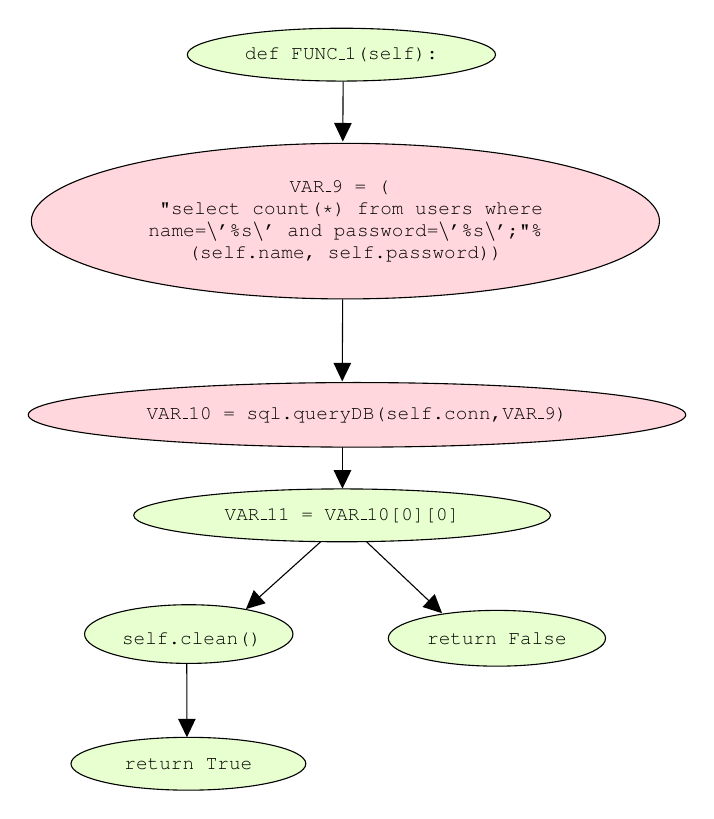
\begin{tikzpicture}[x=0.75pt,y=0.75pt,yscale=-1,xscale=1]
%uncomment if require: \path (0,579); %set diagram left start at 0, and has height of 579

%Straight Lines [id:da40486194850629165] 
\draw    (350.33,84.44) -- (350.18,110.31) ;
\draw [shift={(350.17,113.31)}, rotate = 270.33] [fill={rgb, 255:red, 0; green, 0; blue, 0 }  ][line width=0.08]  [draw opacity=0] (8.93,-4.29) -- (0,0) -- (8.93,4.29) -- cycle    ;
%Straight Lines [id:da3558101395642197] 
\draw    (350.11,189.33) -- (349.91,225.89) ;
\draw [shift={(349.89,228.89)}, rotate = 270.32] [fill={rgb, 255:red, 0; green, 0; blue, 0 }  ][line width=0.08]  [draw opacity=0] (8.93,-4.29) -- (0,0) -- (8.93,4.29) -- cycle    ;
%Straight Lines [id:da1153108036201882] 
\draw    (350,257.83) -- (350,277.58) ;
\draw [shift={(350,280.58)}, rotate = 270] [fill={rgb, 255:red, 0; green, 0; blue, 0 }  ][line width=0.08]  [draw opacity=0] (8.93,-4.29) -- (0,0) -- (8.93,4.29) -- cycle    ;
%Straight Lines [id:da9689031534825849] 
\draw    (339.44,306.22) -- (305.73,336.58) ;
\draw [shift={(303.5,338.58)}, rotate = 318] [fill={rgb, 255:red, 0; green, 0; blue, 0 }  ][line width=0.08]  [draw opacity=0] (8.93,-4.29) -- (0,0) -- (8.93,4.29) -- cycle    ;
%Straight Lines [id:da36506589920381805] 
\draw    (361.67,306.22) -- (395.82,338.52) ;
\draw [shift={(398,340.58)}, rotate = 223.4] [fill={rgb, 255:red, 0; green, 0; blue, 0 }  ][line width=0.08]  [draw opacity=0] (8.93,-4.29) -- (0,0) -- (8.93,4.29) -- cycle    ;
%Straight Lines [id:da5712758559994653] 
\draw    (275,364.22) -- (275.05,397.36) ;
\draw [shift={(275.06,400.36)}, rotate = 269.91] [fill={rgb, 255:red, 0; green, 0; blue, 0 }  ][line width=0.08]  [draw opacity=0] (8.93,-4.29) -- (0,0) -- (8.93,4.29) -- cycle    ;

% Text Node
\draw  [fill={rgb, 255:red, 232; green, 255; blue, 207 }  ,fill opacity=1 ]  (349.5, 71.46) circle [x radius= 74.25, y radius= 12.73]   ;
\draw (349.5,71.46) node  [font=\scriptsize] [align=left] {\begin{minipage}[lt]{71.4pt}\setlength\topsep{0pt}
\begin{center}
{\fontfamily{pcr}\selectfont def FUNC\_1(self):}
\end{center}

\end{minipage}};
% Text Node
\draw  [fill={rgb, 255:red, 255; green, 215; blue, 220 }  ,fill opacity=1 ]  (351.42, 151.67) circle [x radius= 151.32, y radius= 37.48]   ;
\draw (351.42,151.67) node  [font=\scriptsize] [align=left] {\begin{minipage}[lt]{145.41pt}\setlength\topsep{0pt}
\begin{center}
{\fontfamily{pcr}\selectfont VAR\_9 = ( \ \ }\\{\fontfamily{pcr}\selectfont  \ "select count(*) from users where 		name=\textbackslash '\%s\textbackslash ' and password=\textbackslash '\%s\textbackslash ';"\% (self.name, self.password))}
\end{center}

\end{minipage}};
% Text Node
\draw  [fill={rgb, 255:red, 255; green, 215; blue, 220 }  ,fill opacity=1 ]  (357, 245) circle [x radius= 158.39, y radius= 15.56]   ;
\draw (357,245) node  [font=\scriptsize] [align=left] {\begin{minipage}[lt]{152.32pt}\setlength\topsep{0pt}
\begin{center}
{\fontfamily{pcr}\selectfont VAR\_10 = sql.queryDB(self.conn,VAR\_9)}
\end{center}

\end{minipage}};
% Text Node
\draw  [fill={rgb, 255:red, 232; green, 255; blue, 207 }  ,fill opacity=1 ]  (275.95, 350.62) circle [x radius= 50.2, y radius= 14.14]   ;
\draw (275.95,350.62) node  [font=\scriptsize] [align=left] {\begin{minipage}[lt]{48.21pt}\setlength\topsep{0pt}
\begin{center}
{\fontfamily{pcr}\selectfont  self.clean()}
\end{center}

\end{minipage}};
% Text Node
\draw  [fill={rgb, 255:red, 232; green, 255; blue, 207 }  ,fill opacity=1 ]  (424.42, 352.65) circle [x radius= 52.33, y radius= 13.44]   ;
\draw (424.42,352.65) node  [font=\scriptsize] [align=left] {\begin{minipage}[lt]{50.58pt}\setlength\topsep{0pt}
\begin{center}
{\fontfamily{pcr}\selectfont return False}
\end{center}

\end{minipage}};
% Text Node
\draw  [fill={rgb, 255:red, 232; green, 255; blue, 207 }  ,fill opacity=1 ]  (349.83, 293.42) circle [x radius= 100.41, y radius= 12.73]   ;
\draw (349.83,293.42) node  [font=\scriptsize] [align=left] {\begin{minipage}[lt]{96.79pt}\setlength\topsep{0pt}
\begin{center}
{\fontfamily{pcr}\selectfont VAR\_11 = VAR\_10[0][0]}
\end{center}

\end{minipage}};
% Text Node
\draw  [fill={rgb, 255:red, 232; green, 255; blue, 207 }  ,fill opacity=1 ]  (275.78, 413.1) circle [x radius= 56.57, y radius= 12.73]   ;
\draw (275.78,413.1) node  [font=\scriptsize] [align=left] {\begin{minipage}[lt]{54.25pt}\setlength\topsep{0pt}
\begin{center}
{\fontfamily{pcr}\selectfont return True}
\end{center}

\end{minipage}};


\end{tikzpicture}
    \caption{A visualization of a CFG (Control Flow Graph) that has been constructed from the function gadget shown in figure \ref{fig:func_gadget}. The nodes in the graph that have a red background represent vulnerable statements, while the nodes with a green background represent normal statements.}
 \label{fig:cfg}
\end{figure}
 \par \textbf{GNN-base model preparation}:  During the training process  each CFG was treated as a function gadget $d_i$ where each node is a statement $s_{ij}$  that has its corresponding label $y_{ij}$. All statements were then fed to one of the feature extractors shown in table \ref{table:Embedding} to generate contextualized dynamic embeddings.  After that, the generated embeddings  went to a GNN-based model to produce final predictions.  The architectures used for baseline GNNs are Graph Convolution Network (GCN)\cite{GCN} and Graph Attention Network (GAT)\cite{GAT}, which was trained to perform node-level classification tasks to detect potentially vulnerable statements.  To fully compare the performance of DetectBERT and GNN approaches, we conducted several experiments on each architecture using various hyperparameters. Each model was trained on the processed dataset for 100 epochs with the training strategy described in section \ref{sec:training}.



\par \textbf{Results}: the results are presented in Figure \ref{fig:RQ3_graphs} and Table \ref{table:RQ3_res}.  The top three plots in Figure \ref{fig:RQ3_graphs} demonstrate that increasing the hidden size has a significant positive impact on the performance of the models, as measured by f1 score, precision, and recall. This finding is consistent across all classifier architectures, except for GAT classifiers that use mpnet as their feature extractor. Specifically, our experiment showed that models with hidden size $h_{mpnet}=784$ have an improvement of around $5.8\%$, $7.2\%$, and $3.9\%$ in f1 score, precision, and recall, respectively over models with lower hidden size $h_{miniLM}=384$. These results are aligned with  findings in the previous RQ1, where  a larger hidden size also results in better performance.
\begin{table}[h]
\centering
\begin{tabular}{llll}
\Xhline{2\arrayrulewidth}
\textbf{Classifier} &\textbf{F1} &\textbf{Prec}&\textbf{Rec}\\
 \hline
\rowcolor{gray!15} 
 GCN & 40.48 $\pm$ 6.70 &34.18 $\pm$ 6.02 &  58.35 $\pm$ 6.35\\
 GAT & 33.75 $\pm$ 16.75  & 29.99 $\pm$ 13.99  & 44.53 $\pm$ 22.59\\
\rowcolor{gray!15} 
 BERT (DetectBERT) & \textbf{64.88 $\pm$ 5.46} & \textbf{60.71 $\pm$ 8.08} &  \textbf{73.08 $\pm$ 2.65}\\
\Xhline{2\arrayrulewidth}
\end{tabular}
\caption{ Performance of DetectBERT and other GNN-based approaches. we can see that DetectBERT outperforms GCN and GAT in both precision and recall.}
\label{table:RQ3_res}
\end{table}
\par The lower plots of Figure \ref{fig:RQ3_graphs} reveal another pattern.  As the number of encoder layers increases, the performance of all GNN-based models tends to decrease across all metrics. This phenomenon is commonly referred to as the over-smoothing\cite{over_smooth} and over-quashing \cite{over_squash} problems, which can arise in the message-passing mechanism of GNN architectures. Over-smoothing occurs when the GNN model aggregates too much information from neighboring nodes, causing the feature vector of each node to lose its unique characteristics and become overly similar to those of its neighbors. As a result, the model may struggle to distinguish between different nodes and make accurate predictions. On the other hand, over-quashing occurs when the GNN model compresses the information obtained from neighboring nodes, leading to the loss of  critical features for making accurate predictions. Despite these issues in GNN-based models, as the number of encoder layers increased, we did observe a  decline in DetectBERT's precision metric. However, the recall metric, which measures the ability of the model to correctly identify all vulnerable statements, was not significantly affected. This suggests that DetectBERT's ability to capture and retain important information from the input was not compromised as the number of encoder layers increased.

\par Overall,  in all metrics, the performance of DetectBERT outshined that of GNN-based models. As we can see in table \ref{table:RQ3_res}, the average F1, precision, and recall scores of DetectBERT are nearly double those of GCN and GAT approaches, with an improvement of more than $160\%$ in the F1 score, $170\%$ in the precision score, and $140\%$ in the recall score.  One possible explanation for this performance difference is  discussed in section \ref{sec:motivation} and figure \ref{fig:model_view}, where the classifier model of DetectBERT creates multiple attention patterns at each attention head of each encoder layer, this resulted in contextualized vectors that represent combination of multiple weighted graph structures. For instance, a DetectBERT classifier with 12 attention heads and a hidden size of 768 is equivalent to incorporating 12 distinct graph structures at each encoder layer, with each node having an embedding vector of size 64 ($768/12 = 64$).
\par In conclusion, these empirical results provide strong evidence in favor of using transformer-based models such as DetectBERT for vulnerable statement classification tasks, especially in scenarios where a larger number of encoder layers are needed to capture complex patterns in the data. By utilizing the power of transformers, we  can avoid the over-smoothing and over-quashing issues often associated with GNN models, while still achieving high levels of accuracy and recall. 


\subsubsection{Experiment results for RQ4}\label{sec:RQ4}
\par \textbf{Data and model preparation}: In this section, we evaluate DetectBERT's ability to detect vulnerabilities in various types of Python statements. First processed statement $s_{ij}$  was  categorized into statement types, such as "Return", "Condition", "For/While", "Assign", "Expression", "Assert", "Import From", "Augmented assignment", "Import", "Function declaration", and "Docstring". To assess the effectiveness of DetectBERT on each type of statement, separate experiments are conducted on two datasets, CVEFixes and VUDENC,  to analyze if the same types of statements are accurately classified as vulnerable in both datasets.  The model architecture trained in the RQ2 experiment was reused and evaluated. Through this analysis, we aim to identify the common types of vulnerable statements that typically contain vulnerable patterns, as well as the degree of agreement between the models and the ground truth labels for each statement type. 
\begin{table}[h]
\centering
\begin{tabular}{lllll}
\Xhline{2\arrayrulewidth}
\textbf{Type} & \textbf{\makecell{Number of\\ statements}} &\textbf{F1} & \textbf{MCC} & \textbf{AUROC}\\
\hline
Condition        & 1660 & 83.99 & 0.8238 & 0.9819\\
\rowcolor{gray!15} 
Return           & 1110 & 87.20 & 0.8767 & 0.9441\\
Assign           & 3524 & 72.42 & 0.6928 & 0.8530\\
\rowcolor{gray!15} 
Expression             & 1697 & 73.07 & 0.6819 & 0.7694\\
For/While             & 251  & 49.96 & 0.8156 & 0.6606\\
\rowcolor{gray!15} 
Assert           & 79   & 41.33 & 0.6986 & 0.5480\\
Import From      & 365  & 33.12 & 0.4163 & 0.4571\\
\rowcolor{gray!15} 
Augmented assignment& 44   & 16.66 & 0.0000 & 0.0000\\
Import           & 115  & 16.66 & 0.0000 & 0.0000\\
\rowcolor{gray!15} 
Function declaration & 67  & 16.62 & 0.0000 & 0.0000\\
Docstring        & 393  & 16.64 & 0.0000 & 0.0000\\
\Xhline{2\arrayrulewidth}
\end{tabular}
\caption{Performance of DetectBERT on each statement type in CVEFixes}
\label{table:RQ4_cve}
\end{table}

\begin{table}[h]
\centering

\begin{tabular}{lllll}
\Xhline{2\arrayrulewidth}
\textbf{Type} & \textbf{\makecell{Number of\\ statements}} &\textbf{F1} & \textbf{MCC} & \textbf{AUROC}\\
\hline
Expression           & 4983 & 69.42 & 0.5852 & 0.9082\\
\rowcolor{gray!15} 
Assign               & 9001 & 62.79 & 0.5940 & 0.9031\\
Return               & 2629 & 51.17 & 0.4768 & 0.8816\\
\rowcolor{gray!15} 
Import  From          & 1122 & 48.87 & 0.4057 & 0.8045\\
For/while            & 756  & 47.52 & 0.5185 & 0.7717\\
\rowcolor{gray!15} 
Condition            & 3613 & 43.85 & 0.4492 & 0.7655\\
Augmented assignment & 170  & 45.43 & 0.6758 & 0.6158\\
\rowcolor{gray!15} 
Import               & 674  & 29.17 & 0.3572 & 0.5503\\
Assert               & 192  & 48.07 & 0.7405 & 0.4998\\
\rowcolor{gray!15} 
Docstring            & 918  & 12.50 & 0.0000 & 0.0000\\
Function declaration & 2827 & 12.48 & 0.0000 & 0.0000\\
\Xhline{2\arrayrulewidth}
\end{tabular}
\caption{Performance of DetectBERT on each statement type in VUDENC}
\label{table:RQ4_VUDENC}
\end{table}


\par \textbf{Results}: Tables \ref{table:RQ4_cve} and \ref{table:RQ4_VUDENC} present the evaluation results of DetectBERT for each statement type from the evaluation subsets of the CVEFixes and VUDENC datasets, respectively. The tables report performance metrics such as F1-score, MCC, and AUROC. The first column in both tables lists the statement type being evaluated, while the second column shows the number of samples available for each statement type. All statements type are arranged based on the AUROC score in the descending order

\par In the CVEFixes dataset, the model performs exceptionally well in detecting vulnerabilities in "Return", "Condition", "For/While", "Assign" and "Expression" statements, as it achieved the highest scores for all metrics. However, the model seems to struggle in identifying vulnerabilities in "Augmented assignment," "Import," "Function declaration," and "Docstring" statements, with scores being very low or zero. This could be attributed to the limited number of samples available for these types of statements or the fact that they are not actually vulnerable, which is a positive signal indicating that the model can distinguish between statements that have the potential to contain vulnerable patterns and the statements that are labeled as vulnerable just because it is deleted in the commits that patch the vulnerable code.

\par On the other hand, the performance metrics in the VUDENC dataset are more evenly distributed due to the larger number of samples available. Nonetheless, the same pattern observed in the CVEFixes dataset can be seen, where the model performs  best in detecting vulnerabilities in "Condition", "Assign", "Expression", "Return", and "For/While" statements with very high AUROC scores.
\par In summary, the performance of DetectBERT is consistent across both datasets. Our approach has shown to be effective in detecting vulnerabilities in specific types of statements such as "Return", "Condition", "For/While", "Assign" and "Expression". These results align with real-world coding environments where these types of statements are more likely to contain vulnerable defects.

\section{Discussion and future works}
This section provides a concise report about the limitations of our DetectBERT approach as well as the potential approaches that can be used in future works.
\subsection{Limitations} \label{sec:limitation}

\subsubsection{Data limitation}
Both VUDENC and CVEFixes datasets used in this study come with their own set of limitations that can affect the validity and generalizability of the model.

\par One limitation of VUDENC is the presence of duplicated data in the train and test datasets, which can lead to data leakage and overfitting during model training. Although we have made efforts to remove duplicate samples by eliminating identical files from commits that patch the same issue, there may still be cases where there are nearly duplicated files due to code reuse practices in different open-source projects. For the  CVEFixes dataset, one limitation is that the number of commits that patch vulnerabilities in Python is still limited, which can limit the ability of the model to generalize over the new and unseen data. Moreover, for the CVEfixes dataset  to be up-to-date the data collection pipeline of CVEFixes  needs to be re-run which might cost more than 3 days for each run. 

\par Another limitation of VUDENC and CVEFixes is that they focus on vulnerabilities that are patched by source code changes, which may not accurately reflect the full range of vulnerabilities present in software systems. Furthermore, the dataset only includes vulnerabilities that have been publicly disclosed and patched, which can bias the results towards known vulnerabilities and overlook other vulnerable patterns that are missed due to commits that partially solve the problem or the developer just overlook the vulnerable issue.

\subsubsection{Data preprocessing pipeline limitation}

\par The DetectBERT model heavily relies on the AST module for its data preprocessing pipeline. However, when it comes to parsing and extracting function gadgets from large files with more than 1000 lines, the AST module can be really slow. This can lead to long processing times, which can limit the range of use cases for the model, especially in situations where fast processing times are necessary, such as in real-time or low-latency applications. Moreover, the AST module for Python3 cannot parse source code from older Python versions, limiting the scalability of our approach. 
\par Additionally, another issue with the data preprocessing pipeline is that the files are parsed into function gadgets, which also limits the context of the SVD model to a functional unit. This can make it challenging for the model to detect more complex or nuanced vulnerabilities that require a broader context or reasoning from other functions.

\subsubsection{Model limitation}
\par Overall, DetectBERT is a versatile approach to detecting software vulnerabilities using only BERT-based language models. However, there are still some limitations to be aware of when using this model.

\par  One key limitation of DetectBERT is its computational complexity, which is primarily caused by the self-attention layers. The model includes two layers that contain multiple transformer encoders, resulting in a significant demand for computational resources during both training and inference. The high computational complexity can limit the scalability of the model and make it less accessible to researchers and developers who do not have access to powerful computing resources.

\par While DetectBERT has shown promising results in the  SVD  task for SAST,  another limitation is that DetectBERT may not be suitable for all types of software vulnerability detection tasks. Particularly, our approach is not suitable to be used in real-time or low-latency applications (e.g in IoT devices) where speed and efficiency are critical.

\label{sec:con1}



\subsection{Future works}
\label{sec:con3}
DetectBERT has shown promising results in the SVD task, however, there is  still a lot of room for improvement. In this section,  We will discuss potential approaches for future work that can be categorized into two groups: data-centric approaches and model-centric approaches.
\subsubsection{Data-centric improvement}

\par To enhance the efficiency and scalability of DetectBERT, exploring alternative data preprocessing methods could be a promising approach. Currently, the model relies heavily on the AST module, which may be time-consuming and inefficient when extracting function gadgets from large files. Future research could investigate the use of other parsing techniques or tools that offer faster processing times. Another potential solution is to incorporate part-of-speech (POS) tagging, a technique used in NLP to tag sentences or words in a paragraph by analyzing the context. 

\par Another important area of improvement is the availability of training data for different programming languages. While there is a significant amount of publicly available data for C/C++ \cite{sard, devign, SATE, Draper, Are, Linevd, nvd}, datasets for other programming languages are still limited. Future research should focus on collecting more diverse training data to better train and evaluate the model's ability to detect vulnerabilities in different programming languages. It may also be possible to improve the performance of the model by applying data augmentation techniques such as adding noise perturbations  (replace variables, function names, and strings) to the training data and generating a larger and more diverse set of training data.

\subsubsection{Model-centric improvement}

To further improve the performance of the DetectBERT model, several possible alternative architectures and training strategies can be explored in future research.

One approach that could be considered is utilizing different variants of BERT such as ALBERT\cite{albert}, DistilBERT\cite{distilbert} or other transformer-based architecture such as  XLNet\cite{xlnet}, Reformer\cite{reformer}, Longformer\cite{longformer} and Perceiver\cite{perceiver}, that are designed to reduce the space and enhance the speed of the model. In addition, other pre-train strategies for feature extractors could also be explored to further enhance the performance of the DetectBERT model. One potential approach is utilizing contrastive learning objectives \cite{constrastive_learn} to pre-train the model for the SVD task. This involves comparing two or more code statements and minimizing the statements that have the same labels while maximizing the distance between the same that have different labels.

In our study,  we focused on removing the need to construct graphs for source code in the SVD task. However, recent research has explored the use of transformer architecture on graph data and achieved impressive results in tasks that require graphs as the underlying data structure. Notable previous works include Graph Transformer\cite{graph_trans}, Spectral Attention Networks\cite{spectral}, Graph Relative Positional Encoding Transformer\cite{GRPE}, Edge Augmented Transformer\cite{EGT}, Graphormer\cite{graphormer} and TokenGT \cite{tokengt}. By utilizing transformers for graphs, researchers have the potential to overcome some limitations of graph neural networks, such as scaling to larger and denser graphs and increasing model size without over-smoothing.



\section{Related work}
\begin{table*}[h]
\centering
\begin{tabular}{lllllll}
\Xhline{2\arrayrulewidth}
\textbf{Name} & \textbf{Dataset} &  \textbf{Model used} & \textbf{Model type} &  \textbf{Granularity} & \textbf{Language}\\ [0.5ex] 
\hline
\rowcolor{gray!15} 
Vuldeepeeker (2018)\cite{vuldeekeeper} & SARD\cite{sard} + Draper\cite{Draper} & Word2vec\cite{word2vec} + BLSTM\cite{LSTM} & Sequence & Slice & C/C++\\ 
$\mu$Vuldeepeeker (2018)\cite{vuldeekeeper} & SARD\cite{sard} + Draper\cite{Draper} & Word2vec\cite{word2vec} + BLSTM\cite{LSTM} & Sequence & Slice & C/C++\\ 
\rowcolor{gray!15} 
SySeVR (2018)\cite{SySeVR} & SARD\cite{sard} + Draper\cite{Draper} & word2vec\cite{word2vec} + BLSTM\cite{LSTM} & Sequence & Slice & C/C++ \\ 
VulDeeLocator (2020) \cite{VulDeeLocator} & SARD\cite{sard} + NVD\cite{nvd} & Word2vec\cite{word2vec} + BGRU\cite{GRU} & Sequence & Slice & C/C++\\ 
\rowcolor{gray!15} 
VUDENC (2022)\cite{VUDENC} & VUDENC\cite{VUDENC} & Word2vec\cite{word2vec} + LSTM\cite{LSTM} & Sequence & Slice & Python\\ 
Devign (2019)\cite{devign} &  Devign\cite{devign} & Word2vec\cite{word2vec} + GGNN \cite{GGNN}& Graph & Function & C/C++\\ 
\rowcolor{gray!15} 
Reveal (2020)\cite{Are} &  Reveal\cite{Are} & Word2vec\cite{word2vec} + GGNN\cite{GGNN} & Graph & Function & C/C++\\ 
DeepWukong (2021)\cite{DeepWukong} & SARD\cite{sard} + Redis + Lua &  Doc2Vec\cite{doc2vec} + GCN/GAT\cite{GCN,GAT} &  Graph & Function & C/C++\\ 
\rowcolor{gray!15} 
IVdetect (2021)\cite{IVDetect} & SARD\cite{sard} + NVD\cite{nvd} &  GloVe\cite{glove} + GRU\cite{GRU} + FA-GCN\cite{IVDetect} &  Graph & Statement & C/C++\\ 
Linevd (2022)\cite{Linevd} & Big-Vul\cite{Linevd} &  CodeBERT\cite{codebert} + GAT/GCN\cite{GCN,GAT} & Graph & Statement & C/C++\\ 
\rowcolor{gray!15} 
MVD (2022)\cite{MVD} &  MVD\cite{MVD} &  Doc2Vec\cite{doc2vec} + FS-GNN\cite{MVD} & Graph & Statement & C/C++\\ 
 DetectBERT (2023) & VUDENC\cite{VUDENC} + CVEfixes\cite{cvefixes} & BERT variants\cite{mpnet,codebert,minilm} + BERT\cite{bert} & Transformers & Statement & Python\\ 
\Xhline{2\arrayrulewidth}
\end{tabular}
\caption{A summary of the different deep learning approaches used in recent years (from 2018 to 2022), including the type of embedding and model architecture employed in each study, as well as the datasets utilized for training and evaluation.}
\label{table:related_work}
\end{table*}

\par  We introduce this section to provide a comprehensive overview of the use of deep learning techniques for vulnerability detection in recent years (from 2018 to 2022), to help position our work in the larger context of the field. We will focus mainly on two perspectives: the architecture of the deep learning model and the level of granularity of these works.

\subsection{Sequence-based models}
\par  Sequence-based/RNN-based models, such as LSTM\cite{LSTM}, GRU\cite{GRU}, Bidirectional-LSTM(BiLSTN), and Bidirectional-GRU(BiGRU), have been extensively used for analyzing sequence or time-series data. In the domain of detecting vulnerabilities in source code, the data is typically partitioned into code slices where all slices are tokenized into a sequence of tokens and then fed to an RNN-based model. Since most previous works\cite{vuldeekeeper,vuldeepeeker2,SySeVR,VulDeeLocator,VUDENC} for slice-level SVD are performed using the same kind of architecture (LSTM, GRU) and embedding method. Typically,  static embedding techniques, such as word2vec\cite{word2vec}, are often employed to extract representation vectors, which are then fed into an RNN-based model, like BiLSTM or BiGRU, for classification. Therefore, many approaches have a data-centric methodology, where different techniques are used in the data preprocessing steps to enhance the final performance of the model. 

\par For instance, Vuldeepeeker\cite{vuldeekeeper} obtains library/API function calls from training programs, consolidates relevant program "slices", tokenizes them, applies a trained Word2Vec\cite{word2vec} model, and then employs a BiLSTM for binary classification. On the other hand, $\mu$Vuldeepeeker\cite{vuldeepeeker2} introduces the concepts of "code attention" using code slices to capture local and global information and combine them to obtain a complete feature representation.  The intuition behind "slices" in these studies  is based on the idea that only certain lines of code are essential for predicting vulnerabilities. Therefore, instead of analyzing the entire code, slices from "interesting points" such as API calls, array indexing, and pointer usage are considered for prediction, while the rest of the code is excluded.
\par  SysSeVR\cite{SySeVR} presents a framework for automatically extracting Syntax-based Vulnerability Candidates (SyVCs) and Semantics-based Vulnerability Candidates (SeVCs). SyVCs refer to pieces of code in a program that may be vulnerable based on syntax analysis, while SeVCs extend to incorporate other semantically related statements. Similarly, VulDeeLocator\cite{VulDeeLocator} also leverages program analysis and deep learning techniques to generate SeVCs and remove false positives by extracting tokens from the source code based on SyVCs. The intermediate code is used to identify semantically related statements, which are encoded into vectors and then employed to train a neural network for vulnerability detection. The resulting output specifies the vulnerability location, yielding a more precise outcome. As far as we know, VUDENC\cite{VUDENC} is the only work that has developed a solution for detecting vulnerabilities in Python code. VUDENC uses tokenization to extract overlapping code slices, where each slice consists of 200 tokens. The authors employ word2vec and LSTM for feature extraction and classification.


\subsection{Graphs-based models}
\par Recent years have witnessed a surge in the popularity of graph neural network (GNN)-based methods for detecting vulnerable patterns in source code. These methods use graph structures that represent statements as nodes, thereby enabling the combination of feature vectors of each statement and its neighbors. Unlike slice-level methods, which consider feature vectors in isolated slices, GNN-based methods explicitly train feature vectors of each statement combined with contextual features such as edges and neighbor nodes, thereby potentially enhancing the model's ability to detect relevant patterns. To the best of our knowledge, GNN-based methods are currently considered the dominant approach in this field and have been found to achieve state-of-the-art results. Here we will only mention some of the most notable studies


\par For function-level vulnerable code detection, there are approaches such as Devign\cite{devign} and Reveal\cite{Are}, that focus on detecting vulnerabilities at the function level. These approaches utilize word2vec in conjunction with Gated Graph Recurrent Layers (GGNN) \cite{GGNN} to generate embedding vectors from various graph structures, including Abstract Syntax Trees (AST), Code Property Graphs (CPG), Control Flow Graphs (CFG), Data Dependencies Graphs (DDG), Data Flow Graphs (DFG), and Natural Code Sequences (NCS).  DeepWukong \cite{DeepWukong} is another approach for detecting bugs in software programs, which first constructs a Program Dependence Graph based on control flow and data-flow information. It then generates subgraphs or slices of the PDG using forward and backward traversal starting from a program point of interest. During the detection phase, control and data dependencies of a target program are extracted, symbolized, and embedded by Doc2Vec\cite{doc2vec} to feed into trained GNNs like GCN\cite{GCN} or GAT\cite{GAT} models for graph classification.

\par Recently, there has been an increasing focus on the use of Graph Neural Networks (GNNs) to achieve statement-level classification for identifying software vulnerabilities. One prominent example of this approach is IVDetect\cite{IVDetect}, which uses a Program Dependence Graph (PDG) to differentiate vulnerable code from surrounding contextual code. IVDetect then employs a Graph Convolution Network (GCN)\cite{GCN} with feature-attention (FA-GCN) to perform graph-based classification. The GNNExplainer\cite{GNExplainer} is also utilized to identify crucial program dependencies and statements that are most relevant to the detected vulnerability. Another model, LineVD\cite{Linevd}, takes a single function of source code as input and processes it into individual statements. This model uses CodeBERT \cite{codebert}to separately embed both function-level and statement-level codes and focuses on data and control dependency information. These features are then fed into GAT or GCN for training and inference. Finally, MVD\cite{MVD} is a method for memory-related vulnerability detection that constructs a PDG with additional semantic information from a Call Graph and reduces noise by conducting program slicing. The statements of each slice are transformed into low-dimensional vector representations using Doc2Vec, and Flow-Sensitive Graph Neural Networks (FS-GNN) are used to learn vulnerability patterns for vulnerability detection at the statement level. These models offer promising avenues for future research in the field of software vulnerability detection.
\subsection{Position of our approach}
Our approach DetectBERT can achieve the statement level of granularity without relying on any kind of graph structure. For the features extractor, we used the BERT-based models \cite{mpnet,minilm,sbert} that are pre-trained on multiple programming languages to benefit from the power of transfer learning. The output of the feature extractor is concatenated and fed to another series of encoder blocks to learn the contextual relationship between statements in a Python function.


\section{Conclusion}

In this paper, we introduced DetectBERT, a novel architecture that utilizes the self-attention mechanism to detect vulnerable code at the statement level in multiple programming languages. Unlike existing methods that rely on predefined graph structures, DetectBERT is flexible and able to capture contextual interactions between statements. To evaluate its effectiveness, the authors created a new dataset by extracting and normalizing statements from real-world open-source Python projects, resulting in a total of 211,317 statements. Empirical results demonstrate that DetectBERT outperforms other graph-based methods that rely on control flow graphs (CFGs), achieving an average F1 score of 64.88\%, precision of 60.71\%, and recall of 73.08\% for Python. Moreover, the data normalization step also enhances the model's ability to generalize to new, unseen data and increases its robustness against adversarial attacks. In the near future, we are planning to develop our own datasets for multiple programming languages with fewer duplicated samples for better evaluation and further improve the model's performance.
\bibliography{mybib} 
\bibliographystyle{ieeetr}

\EOD
\begin{figure*}[h]
    \centering
    \includegraphics[width=0.97\textwidth, align=center]{attention_heads.png}
    \caption{BERTViz \cite{bertviz} is used to visualize attention patterns for each head in a classifier model that contains 6 encoder layers, represented by columns and rows respectively. Here lines that are bolder imply higher attention weights. Each cell in the figure contains a thumbnail version for each head of the following figure \ref{fig:attention_view}, which is specific to the input statements $s_{i}$ of function gadget $\mathbf{d}_i$, which is depicted in figure \ref{fig:func_gadget}.}
    \label{fig:model_view}
\end{figure*}
\section{Appendices}
\subsection{Inside the classifier model of DetectBERT} \label{sec:behind_the_scene}
\par In order to understand how the DetectBERT classifier model identifies vulnerable statements, we will examine a use case involving the function gadget shown in Figure \ref{fig:func_gadget}. This function contains statements that are susceptible to SQL injection attacks. Specifically, statements 2 and 3 can be exploited by an attacker who manipulates the input parameters self.name and self.password to insert malicious SQL code into the query. The DetectBERT model used in this experiment used mpnet as the feature extractor and the classifier contain  6 layers of transformers encoder. Figure \ref{fig:model_view} is an illustration of all attention weights that are assigned between each pair of statements in the sample function gadget.

\par From figure \ref{fig:model_view},  it is clear that  by stacking multiple encoder layers that utilize multi-head self-attention mechanisms, the DetectBERT model is able to form various attention patterns in each head, which allows it to cover a wider range of relationships between statements than GNN-based approaches with pre-defined graph structures. Taking a closer look at the way the conditional statement $s_{i5}$ focuses on other statements in figure \ref{fig:attention_view}, we can see that most of the attention heads are able to recognize the two most important statements in the function gadget (number $s_{i2}$ and $s_{i3}$), which contain the SQL statement and are also the center of data-flow and control-flow in this function. Other heads, such as the red and brown heads, tend to pay attention to the two statements that are influenced by the current conditional statement. This insight also shows us that positional encoding has done its job very well.



\begin{figure}[h]
  \centering
    \includegraphics[width=80mm, align=center]{attention_heads_details.png}
    \caption{A visualization generated by BERTViz\cite{bertviz} that shows how the conditional statement $s_{i5}$ gathers contextualized information from other statements  }
    \label{fig:attention_view}
\end{figure}
 \par In figure \ref{fig:model_view}, it is also noteworthy that at every attention head, as  the contextualized embeddings go to the deeper layer, the attention patterns seem to just focus on the two specific statements which are also the statement that contains vulnerable code.  According to a previous study conducted by Clark et al \cite{bert_insignt}, this phenomenon also means that the models can not find anything else to attend to and choose to bypass the current self-attention layer by choosing to gather the same embedding features as the previous layers. From this intuition, we can easily see that all  heavy-lifting jobs are actually done in the first few layers, and increasing more encoder layers in the classifier models is not necessary. In fact, this might also lead to the overfitting problem which is demonstrated in RQ1.
 \begin{figure*}[h]
    \centering
    

\tikzset{every picture/.style={line width=0.75pt}} %set default line width to 0.75pt        

\begin{tikzpicture}[x=0.75pt,y=0.75pt,yscale=-1,xscale=1]
%uncomment if require: \path (0,579); %set diagram left start at 0, and has height of 579

%Image [id:dp2901992266768938] 
\draw (226.89,227.01) node  {\includegraphics[width=205.84pt,height=204.51pt]{wo_mask.png}};
%Image [id:dp850445924774881] 
\draw (557.49,227.08) node  {\includegraphics[width=205.27pt,height=204.62pt]{w_mask.png}};
%Straight Lines [id:da3262834651605835] 
\draw    (393.46,122.26) -- (393.97,354.06) ;

% Text Node
\draw (172.72,373.64) node [anchor=north west][inner sep=0.75pt]  [font=\scriptsize] [align=left] {Before normalization};
% Text Node
\draw (508.31,373.64) node [anchor=north west][inner sep=0.75pt]  [font=\scriptsize] [align=left] {After normalization};


\end{tikzpicture}
    \caption{ The t-SNE algorithm is utilized to visualize the 2D scatter plots of the final embedding vectors of all statements ($s_{ij}$) in the augmented test set. These embedding vectors are generated by the last layer of the encoder model, which has a hidden size of 786, before being projected and classified. Each statement is assigned an `x`  marker with  specific color which represent the ground truth label of the current statement} 
    \label{fig:embeddings_visualize}  
\end{figure*}
\subsection{The effect of code normalization}\label{sec:code_normalization_insight}
In section is denoted to provide insights about how the code normalization steps described in section \ref{sec:FE} can help the model better resist adversarial attacks. The models  used in RQ2 are utilized to generate embeddings for  visualization.


\par  The visualization presented in figure \ref{fig:embeddings_visualize} reveals that both models attempted to differentiate between vulnerable and non-vulnerable statements by separating their embeddings into distinctive regions. The unnormalized code-trained model produced clearer and more isolated clusters of vulnerable embeddings, forming "islands" within the plot, while the normalized code-trained model pushed vulnerable embeddings toward the edges of the two-dimensional planes. 
\par These findings elucidate why the model trained on unprocessed data achieved higher precision scores, as the isolated "islands" provided a clear boundary to distinguish between vulnerable and non-vulnerable statements. However, the unnormalized code-trained model tended to be overfitted by irrelevant features leading to several false negative cases being missed, which are represented by non-grey markers that are scattered all over the plot. 
 \par In contrast, the normalized-trained model  was able to identify the underlying patterns and structure of the code, despite the presence of irrelevant features. By removing inconsistencies such as variable and method names,  we can better enhance the model to map statements using the same  API calls, and function calls  into unified vectors that are closer to each other in the vector space. Furthermore, the vulnerable embeddings produced by the normalized model were more prone to being pushed toward the right of the plot.   This also explains why the model trained on normalized code achieved higher recall  and AUROC scores. 
\subsection{The performance of DetectBERT on C/C++}\label{sec:C++}
As C/C++ is widely used in previous studies for the source code vulnerability detection task, we also include this section to assess the effectiveness of DetectBERT on a dataset specifically designed for C/C++ programming language and compare its performance with another approach that operates at the same level of granularity ( statement-level). 
 \par \textbf{Baseline}: In this experiment, the observed results in LineVD \cite{Linevd} is used as a baseline for comparison which is shown in table \ref{table:RQ5_exp_res}. For a brief background, in LineVD, they  extracted statements and constructed  program dependency graphs (PDG)  by combining data flow and control flow relationships between statements. After that, all statements are fed into the CodeBERT \cite{codebert} model for statement-level and function-level feature extraction. Finally,  the generated embeddings are then fed to a GAT or GCN to learn the contextualized information based on the built PDG.  Table \ref{table:RQ5_2}  showed the impact of different experimental settings, as reported in the original paper Linevd\cite{Linevd}, on the performance of graph neural network (GNN) models. The results suggest that using the graph attention network (GAT) for feature learning from program dependence graph (PDG) information is the most effective choice. 
\begin{table}[h]
\centering

\label{table:data_stat_c}
\begin{tabular}{lll}
\Xhline{2\arrayrulewidth}
\textbf{} & \textbf{No of function gadgets} & \textbf{No of statements} \\
\hline
Non vulnerable & 14858 & 1030313\\ 
Vulnerable  & 12460 & 31857 \\ 
\Xhline{2\arrayrulewidth}
\end{tabular}
\caption{ In the Devign dataset, the curators did not classify the vulnerability type for each sample, however, most vulnerabilities are memory-related, like buffer overflow, memory leak, crash, and corruption. To extract statements and build function gadgets from C/C++ code,  the PyClang module is used to extract ASTs. Each function gadget is then marked as vulnerable if it contains at least one vulnerable statement, and all statements are labeled using the sample data preprocessing pipeline described in section \ref{sec:FE}. }
\end{table} 
\par \textbf{Data preparation}: The dataset used in LineVD is Big-Vul which comprises source code from multiple open-source projects. However, due to time and resource constraints, we were only able to run DetectBERT on the public Devign dataset\cite{devign}. The data preprocessing pipeline used in this experiment was similar to the one used for Python, as described in the previous section \ref{sec:FE}. To extract and standardize statements, PyClang was utilized to obtain the AST for C/C++ code. As the dataset and data processing methods are different, no conclusions can be drawn regarding the performance of DetectBERT versus LineVD. The experimental outcomes presented herein are solely for demonstration and reference purposes. The preprocessed Devign dataset can be found on our Huggingface hub: \url{https://huggingface.co/datasets/EddieChen372/devign_with_norm_vul_lines}

  
\begin{table}[h]
\centering

\begin{tabular}{lllll}
\Xhline{2\arrayrulewidth}
\textbf{Model} \& \textbf{Graph Type} & \textbf{F1} & \textbf{R}ec & \textbf{Prec} & \textbf{AUROC} \\
 \hline
\rowcolor{gray!15} 
GAT+CDG & 11.5 & 12.0 & 11.2 & 0.657 \\
GAT+CDG+Func & 30.4 & 49.1 & 22.1 & 0.907\\
\rowcolor{gray!15} 
GAT+PDG & 15.0 & 25.4 & 12.1 & 0.703 \\
GAT+PDG+Func & \textbf{36.0} & 53.3 & \textbf{27.1} & 0.913\\
\rowcolor{gray!15} 
GCN+CDG & 8.4 & 14.3 & 6.0 & 0.632 \\
GCN+CDG+Func & 28.3 & \textbf{55.8} & 19.0 & 0.911 \\
\rowcolor{gray!15} 
GCN+PDG & 8.5 & 12.5 & 6.7 & 0.599 \\
GCN+PDG+Func & 31.0 & 46.0 & 23.5 & 0.905\\
\rowcolor{gray!15} 
No GNN & 12.9 & 16.6 & 10.6 & 0.666 \\
No GNN+Func & 29.6 & 53.7 & 20.5 & \textbf{0.921} \\
\hline
\rowcolor{gray!15} 
Average & 21.1 & 33.8 & 15.8 & 0.780 \\
\Xhline{2\arrayrulewidth}
\end{tabular}
\caption{Performance of GCN and GAT that has been trained and evaluated on Big-Vul dataset to perform node classification task on CDG and PDG. CDG is short for graph control dependency graph which utilizes only control-flow information, while program dependency graph(PDG) applied both data-flow and control-flow knowledge to build graphs from functions.\cite{Linevd}}
\label{table:RQ5_2}
\end{table}

\par \textbf{Model preparation}: Two versions of CodeBERT \cite{codebert, zhou2023codebertscore} were used  for feature extraction. The first version is the same model used in LineVD and the other is particularly pre-trained  for C/C++ programming languages. The classifier model is a BERT model that contains three transformer encoder layers.  The architecture and training strategy  is described in section \ref{sec:training} and figure \ref{fig:train}

\par \textbf{Results}: We conducted training of two versions of DetectBERT using the preprocessed Devign dataset for 100 epochs, and the performance outcomes are presented in Table \ref{table:RQ5_exp_res}. The empirical results indicate that utilizing a  feature extractor that is pre-trained in C/C++ leads to better outcomes. Although the overall performance is still low, DetectBERT still demonstrated promising performance in comparison to the empirical results presented in Table \ref{table:RQ5_2}. Specifically, the best DertBERT version attained an F1 score of 31.17\% and an AUROC score of 0.760, which is comparatively good in comparison to the other GNN-based models used in LineVD (with an average F1 score of 21.1 and AUROC score of 0.780). In future research, we plan to expand our evaluation by testing DetectBERT with other publicly available C/C++ datasets to establish a more comprehensive benchmark against other GNN-based approaches designed for C/C++.

\begin{figure}[h!]
  \centering
    \includegraphics[width=80mm, align=center]{c_sample.png}
    \caption{Our model detected a statement that may be vulnerable  to  CWE-119 (buffer overflow) or CWE-787 (out-of-bounds read or write) . Specifically, the statement in line 116, which is marked as vulnerable, allocates a block of memory of size `slice->data\_size` using the `av\_malloc` function. If the allocation fails, the function returns an error `(AVERROR(ENOMEM))`, and the program will free slice and return an error code. However, if `slice->data\_size` is a very large value (for example, if an attacker can control the input to the function), the `av\_malloc` function may fail to allocate enough memory and return a `NULL` pointer. If the program does not handle this error condition properly, it could lead to a buffer overflow or other memory-related vulnerabilities. Therefore, it is important to ensure that the size of the memory block being allocated is within a reasonable range and to check for errors returned by memory allocation functions.}
    \label{fig:c_sample}
\end{figure}
\begin{table}[h]
\centering
\begin{tabular}{llllll}
\Xhline{2\arrayrulewidth}
\textbf{Dataset}&\textbf{Model} & \textbf{F1} & \textbf{Prec}&  \textbf{Rec}&  \textbf{AUROC}\\
\hline
\rowcolor{gray!15} 
Big-Vul&LineVD-average &21.1 & 15.8  & 33.8 & \textbf{0.780}\\
Devign&\makecell[align=left]{CodeBERT-base\cite{codebert} + \\ BERT} & 21.2 & 14.5 & \textbf{38.9} & 0.747\\
\rowcolor{gray!15} 
Devign&\makecell[align=left]{CodeBERT-C\cite{zhou2023codeBERTscore} +\\ BERT} &  \textbf{31.2} & \textbf{29.8} & 32.7 & 0.760\\
\Xhline{2\arrayrulewidth}
\end{tabular}

\caption{Performance of DetectBERT on the Devign dataset compare to the average performance of GNN-based models trained on the Big-Vul dataset in LineVD\cite{Linevd}.  We can see  that DetectBERT achieved competitive performance in every metric.  Particularly, the best DetectBERT model outperforms models used in LineVD in term of the precision score. }
\label{table:RQ5_exp_res}
\end{table}
\end{document}

